\documentclass[12pt]{amsart}
\usepackage{graphicx, framed,multicol}
\usepackage[shortlabels]{enumitem}
\usepackage{comment}
\usepackage{amscd}
\usepackage{amssymb,xcolor,graphicx}
\usepackage[all, knot]{xy}
\usepackage[top=1.2in, bottom=1.2in, left=1.2in, right=1.2in]{geometry}
\xyoption{all}
\xyoption{arc}
\usepackage{hyperref}

%%\usepackage[notcite,notref]{showkeys}


\def\floor#1{\lfloor #1 \rfloor}








\def\ku{ku}
\def\bbu{\bf bu}
\def\KR{K{\mathbb R}}

\def\CW{\underline{CW}}
\def\cP{\mathcal P}
\def\cE{\mathcal E}
\def\cL{\mathcal L}
\def\cJ{\mathcal J}
\def\cJmor{\cJ^\mor}
\def\ctJ{\tilde{\mathcal J}}
\def\tPhi{\tilde{\Phi}}
\def\cA{\mathcal A}
\def\cB{\mathcal B}
\def\cC{\mathcal C}
\def\cZ{\mathcal Z}
\def\cD{\mathcal D}
\def\cF{\mathcal F}
\def\cG{\mathcal G}
\def\cO{\mathcal O}
\def\cI{\mathcal I}
\def\cS{\mathcal S}
\def\cT{\mathcal T}
\def\cM{\mathcal M}
\def\cN{\mathcal N}
\def\cMpc{{\mathcal M}_{pc}}
\def\cMpctf{{\mathcal M}_{pctf}}
\def\L{\mathbf{L}}
\def \a{\alpha}
\def\b{\beta}
\def\de{\delta}
\def\ds{\displaystyle}
\def\cts{continuous\,}

\def\Mo{Monday}
\def\We{Wednesday}
\def\Fr{Friday}



\def\d{\delta}
\def\td{\tilde{\delta}}

\def\e{\varepsilon}
\def\nsg{\unlhd}




\newcommand{\Q}{\mathbb{Q}}

\newcommand{\bP}{\mathbb{P}}
\newcommand{\bM}{\mathbb{M}}
\newcommand{\A}{\mathbb{A}}
\newcommand{\bH}{{\mathbb{H}}}
\newcommand{\G}{\mathbb{G}}
\newcommand{\bR}{{\mathbb{R}}}
\newcommand{\bL}{{\mathbb{L}}}
\newcommand{\R}{{\mathbb{R}}}
\newcommand{\F}{\mathbb{F}}
\newcommand{\E}{\mathbb{E}}
\newcommand{\bF}{\mathbb{F}}
\newcommand{\bE}{\mathbb{E}}
\newcommand{\bK}{\mathbb{K}}


\newcommand{\bD}{\mathbb{D}}
\newcommand{\bS}{\mathbb{S}}

\newcommand{\bN}{\mathbb{N}}


\newcommand{\bG}{\mathbb{G}}

\newcommand{\C}{\mathbb{C}}
\newcommand{\Z}{\mathbb{Z}}
\newcommand{\N}{\mathbb{N}}

\newcommand{\M}{\mathcal{M}}
\newcommand{\W}{\mathcal{W}}



\newcommand{\itilde}{\tilde{\imath}}
\newcommand{\jtilde}{\tilde{\jmath}}
\newcommand{\ihat}{\hat{\imath}}
\newcommand{\jhat}{\hat{\jmath}}

\newcommand{\fc}{{\mathfrak c}}
\newcommand{\fp}{{\mathfrak p}}
\newcommand{\fm}{{\mathfrak m}}
\newcommand{\fq}{{\mathfrak q}}
\newcommand{\dual}{\vee}


% The following causes equations to be numbered within sections
\numberwithin{equation}{section}


\theoremstyle{plain} %% This is the default, anyway
\newtheorem{thm}[equation]{Theorem}
\newtheorem{preproof}{Preproof Discussion}
\newtheorem{obs}[equation]{Observation}
\newtheorem{thmdef}[equation]{TheoremDefinition}
\newtheorem{introthm}{Theorem}
\newtheorem{introcor}[introthm]{Corollary}
\newtheorem*{introthm*}{Theorem}
%\newtheorem{question}{Question}
\newtheorem*{question}{Question}
\newtheorem{cor}[equation]{Corollary}
\newtheorem{lem}[equation]{Lemma}
\newtheorem{prop}[equation]{Proposition}
\newtheorem{porism}[equation]{Porism}
\newtheorem{algorithm}[equation]{Algorithm}
\newtheorem{axiom}[equation]{Axiom}
\newtheorem*{axioms*}{Axioms}
\newtheorem*{axiom*}{Axiom}
\newtheorem{conj}[equation]{Conjecture}
\newtheorem{quest}[equation]{Question}

\newcommand{\Aug}[3]{\section{#2, August #1, 2024 \quad \S#3}}
\newcommand{\Sept}[3]{\section{#2, September #1, 2024 \quad \S#3}}
\newcommand{\Oct}[3]{\section{#2, October #1, 2024 \quad \S#3}}
\newcommand{\Nov}[3]{\section{#2, November #1, 2024 \quad \S#3}}
\newcommand{\Dec}[3]{\section{#2, December #1, 2024 \quad \S#3}}



\theoremstyle{definition}
\newtheorem{defn}[equation]{Definition}
\newtheorem{chunk}[equation]{}
\newtheorem{ex}[equation]{Example}

\newtheorem{exer}[equation]{Exercise}

\theoremstyle{remark}
\newtheorem{rem}[equation]{Remark}

\newtheorem{notation}[equation]{Notation}
\newtheorem{terminology}[equation]{Terminology}

%%%%%%%%%%%%%
% local definitions
%%%%%%%%%%%%%
\def\TP{\operatorname{TPC}}

\def\HomMF{\operatorname{\uHom_{MF}}}
\def\HomHMF{\operatorname{\Hom_{[MF]}}}

\def\rDsg{D^{\text{rel}}_{\text{sing}}}
\def\Dsg{D_{\text{sing}}}
\def\Dsing{\Dsg}
\def\Db{D^b}


\def\Perf{\operatorname{Perf}}
\def\coh{\operatorname{coh}}

\def\CCh{\check{\cC}}

\newcommand{\Cech}{C}

\newcommand\bs{\boldsymbol}


%\newcommand{\sExt}[4]{\widehat{\operatorname{Ext}}_{#2}^{#1}(#3,#4)}
\newcommand{\cExt}[4]{\uExt_{#2}^{#1}(#3,#4)}

\newcommand\depth{\operatorname{depth}}
\newcommand{\supp}{\operatorname{supp}}

\newcommand{\br}[1]{\lbrace \, #1 \, \rbrace}
\newcommand{\brc}[2]{\lbrace \, #1 \, | \, #2 \rbrace}
\newcommand{\li}{ < \infty}
\newcommand{\quis}{\simeq}
\newcommand{\xra}[1]{\xrightarrow{#1}}
\newcommand{\xla}[1]{\xleftarrow{#1}}
\newcommand{\xroa}[1]{\overset{#1}{\twoheadrightarrow}}
\newcommand{\ps}[1]{\mathbb{P}_{#1}^{\text{c}-1}}

% this is the pull-back of E along l: Z \to X
\newcommand{\pb}[1]{\RQ^*{#1}}
\newcommand{\pbe}{\pb{\cE}}
\newcommand{\YQ}{\gamma}
\newcommand{\RY}{\beta}
\newcommand{\RQ}{\delta}

\newcommand{\mft}[1]{T^{[MF]}_{#1}}
\newcommand{\dst}[1]{T^{\Dsing(R)}_{#1}}

\newcommand{\id}{\operatorname{id}}
\newcommand{\pd}{\operatorname{pd}}
\newcommand{\even}{\operatorname{even}}
\newcommand{\odd}{\operatorname{odd}}

\newcommand{\bl}[1]{{{\color{blue}#1}}}

\def\tmu{\tilde{\mu}}
\def\g{\gamma}
\def\tg{\tilde{\gamma}}
\def\tCliff{\operatorname{\tilde{Cliff}}}
\def\unital{\mathrm{unital}}
\def\D{\Delta}
\def\Tco{\operatorname{T^{\text{co}}}}
\def\Tcob{\operatorname{\ov{T}^{\text{co}}}}

\def\bg{\mathbf g}
\def\ta{\tilde{a}}


\def\z{\zeta}
\def\lf{\operatorname{lf}}
\def\mf{\operatorname{mf}}
\def\lffl{\operatorname{lf}^{\mathrm{fin. len.}}}
\def\mffl{\operatorname{mf}^{\mathrm{fin. len.}}}
\def\len{\operatorname{length}}
\def\Hlf{\operatorname{H}}

\def\codim{\operatorname{codim}}

\def\cPsi{\psi_{\mathrm{cyc}}}
\def\Fold{\operatorname{Fold}}
\def\ssupp{\operatorname{s.supp}}

\def\mult{\operatorname{mult}}
\def\stable{\mathrm{stable}}
\def\and{{ \text{ and } }}
\def\orr{{ \text{ or } }}
\def\oor{\orr}

\def\Perm{\operatorname{Perm}}


\def\Op{\operatorname{Op}}
\def\res{\operatorname{res}}
\def\ind{\operatorname{ind}}

\def\sign{{\mathrm{sign}}}
\def\naive{{\mathrm{naive}}}
\def\l{\lambda}


\def\ov#1{\overline{#1}}

%%%-------------------------------------------------------------------
%%%-------------------------------------------------------------------
% NEW DEFINITIONS BEYOND MARK'S USUAL ONES 
% (OR MODIFIED) 
\newcommand{\chara}{\operatorname{char}}
\newcommand{\Kos}{\operatorname{Kos}}
\newcommand{\opp}{\operatorname{opp}}
\newcommand{\perf}{\operatorname{perf}}

\newcommand{\Fun}{\operatorname{Fun}}
\newcommand{\GL}{\operatorname{GL}}
\def\o{\omega}
\def\oo{\overline{\omega}}

\def\cont{\operatorname{cont}}
\def\te{\tilde{e}}
\def\gcd{\operatorname{gcd}}
%%%-------------------------------------------------------------------
%%%-------------------------------------------------------------------
%%%-------------------------------------------------------------------
%%%-------------------------------------------------------------------
%%%-------------------------------------------------------------------


\def\charpoly{\operatorname{char poly}}
\def\Gal{\operatorname{Gal}}

\makeindex


\begin{document}


\title{Fall 2024 Math 325 Lecture Notes and worksheets}
\maketitle

\setcounter{tocdepth}{1}
\tableofcontents



\Aug{26}{\Mo}{1.1}

%If you are here, you know Calculus. The theory invented in the 18th century by Leibniz and Newton, building off of work of Fermat, took the world by storm after its introduction. Calculus has an incredible ability to solve problems like finding the amount of fuel needed to get a satellite into orbit. And clearly Calculus works, as evidenced by our ability to get satellites into orbit in the real world.

%However, 



What is a number? Certainly the things used to count sheep, money, etc. are numbers:  $1, 2, 3, \dots$.
We will call these the {\em natural numbers}\index{natural number}\index{$\N$} and 
write $\N$ for the set of all natural numbers
$$
\N = \{1, 2, 3, 4, \dots \}.
$$
Since we like to keep track of debts too, we'll allow negatives and $0$, which gives us the {\em integers}\index{integers}\index{$\Z$}:
$$
\Z = \{ \dots, -3, -2, -1, 0, 1, 2, 3, 4, \dots\}.
$$
(The symbol $\Z$ is used since the German word for number is {\em zahlen}.)


Fractions should count as numbers also, so that we can talk about eating one and two-thirds of a pizza last night. We define a {\em rational number}\index{rational number} to be a number expressible
as a quotient of two integers: $\frac{m}{n}$ for $m,n \in \Z$ with $n \ne 0$. For example
$$
\frac{5}{3}, \frac27, \frac{2019}{2020}
$$
are rational numbers. Of course, we often talk about numbers such as
``two and a fourth'', but that the same as $\frac94$. Every integer
is a rational number just by taking $1$ for the denominator; for
example, $7 = \frac{7}{1}$. 
The set of all rational numbers is written as $\Q$ (for ``quotient'').\index{$\Q$} 

You might not havethought about it before, but an expression of the form $\frac{m}{n}$ is really an ``equivalence class'': 
the two numbers $\frac{m}{n}$ and $\frac{a}{b}$ are deemed equal if $mb =
na$. For example $\frac69 = \frac23$ because $6 \cdot 3 = 9 \cdot 2$.



We'll talk more about decimals later on, but recall for now that a decimal that terminates is just another way of representing a rational number. For example,
$1.9881$ is equal to $\frac{19881}{10000}$. Less obvious is the fact that a decimal that repeats also represents a rational number: For example, 
$1.333\dots$ is rational (it's equal to $\frac43$) and so is 
$23.91278278278\dots$. We'll see why this is true later in the semester. 




Are these all the numbers there are? Maybe no one in this class  would answer ``yes'', but the ancient Greeks believed for a time that every number was rational. Let's convince
ourselves, as the Greeks did eventually, that there must be numbers that are not rational. Imagine a square of side length $1$. By the Pythagorean Theorem, the length of
its diagonal, call this number $c$, must satisfy 
$$
c^2 = 1^2 + 1^2 = 2.
$$
That is, there must be a some  number whose square is $2$ since certainly the length of the diagonal in such a square is representable as a number. Right?
Now, let's convince ourselves that there is no {\em rational number} with this property. In fact, I'll make this a theorem.

\begin{thm} There is no rational number whose square is $2$. \index{$\sqrt{2}$}
\end{thm}

\begin{preproof} Before launching a formal proof, let's philosophize
  about how one shows something does not exist. To show something does
  not exist, one proves  that its existence is
  not possible. For example, I know that  there must not be large clump of plutonium sewn into the mattress of my bed. I know this since, if such a clump existed, I'd be
  dead by now, and yet here I am, alive and well!

More generally and formally, one way to prove the falsity of a
statement $P$ is to argue that if we assume $P$ to be true then we can deduce from that
assumption something that is known
to be false. If you can do this, then you have proven $P$ is false. In symbols:
If one can prove
$$
P \Longrightarrow \text{Contradiction}
$$
then the statement $P$ must in fact be false.

In the case at hand, letting  $P$ be the statement ``there is a rational number whose square is $2$'', the Theorem is asserting that $P$ is false. We will prove
this by assuming $P$ is true and deriving an impossibility.

This is known as a proof by contradiction.\index{proof by contradiction}\end{preproof}

\begin{proof} By way of contradiction, assume there were a rational number $q$ such that $q^2 = 2$. By definition of ``rational number'',  
we know that $q$ can be written as  $\frac{m}{n}$ for
some integers $m$ and $n$ such that $n \ne 0$. Moreover, we may assume that we have written $q$ is reduced form so that $m$ and $n$ have no
prime factors in common. In particular, we may assume that not both of $m$ and $n$ are even. (If they
  were both even, then  we could simplify the fraction by factoring out common factors of $2$'s.) Since $q^2 = 2$,
  $\frac{m^2}{n^2} = 2$ and hence $m^2 = 2n^2$. In particular, this shows $m^2$ is even and, since the square of an odd number is odd, it must be that $m$
  itself is even. So, $m = 2 a$ for some integer $a$. But then $(2a)^2 = 2n^2$ and hence $4a^2 = 2n^2$ whence $2a^2 = n^2$. For the same reason as before, this
  implies that $n$
  must be even. But this contradicts the fact that $m$ and $n$ are not both even. 

We have reached a contradiction, and so the assumption that there is a rational number $q$ such that $q^2 = 2$ must be false.
\end{proof}

Thus, if we would like to have a number corresponding to the length of the diagonal of a square with side length one, it must be a number that is real but not rational. Let's record the common name for such a number.

\begin{defn} A real number is \emph{irrational}\index{irrational} if it is not rational.
\end{defn}


A version of the previous proof was known even to the ancient Greeks.


Our first major mathematical goal in the class is to make a formal definition of the real numbers. 
Before we do this, let's record some basic properties of the rational numbers. I'll state this as a Proposition (which is something like a minor version of a Theorem), but we won't prove them; instead, we'll take it for granted to be true based on our own past experience with numbers.

For the rational numbers, we can do arithmetic ($+,-,\times,\div$) and we also have a notion of size $(<,>)$. The first seven observations below describe the arithmetic, and the last three describe the notion of size.


\begin{prop}[Arithmetic and order properties of $\Q$]\label{prop1}
  The set of rational numbers form an ``ordered field''.\label{ordered field} This means that the following ten properties hold:
\begin{enumerate}
\item There are operations $+$ and $\cdot$ defined on $\Q$, so that if $p, q$ are in $\Q$, then so are $p + q$ and $p \cdot q$.
\item Each of $+$ and $\cdot$ is a commutative operation (i.e., $p + q = q + p$ and $p \cdot q = q \cdot p$ hold for all rational numbers $p$ and $q$). 
\item Each of $+$ and $\cdot$ is an associative  operation (i.e., $(p + q) + r = p + (q + r)$ and $(p \cdot q) \cdot r = p \cdot (q \cdot r)$ hold for all rational numbers $p$,
  $q$, and $r$). 
\item The number $0$ is an identity element for addition and the number $1$ is an identity element for multiplication. This means that
 $0 + q = q$ and $1 \cdot q = q$ for all $q \in \Q$. 
\item The distributive law holds: $p \cdot (q + r) = p \cdot q + p \cdot r$ for all $p,q,r \in \Q$. 
\item Every number has an additive inverse: For any $p \in \Q$, there is a number $-p$ satisfying $p + (-p) = 0$.
\item Every nonzero number has a multiplicative inverse: For any $p \in \Q$ such that $p \ne 0$, there is a number $p^{-1}$ satisfying ${p \cdot p^{-1}= 1}$.
\item There is a ``total ordering'' $\leq$ on $\Q$. This means that 
\begin{enumerate}
\item For all $p, q \in \Q$, either $p \leq q$ or $q \leq p$.
\item If $p \leq q$ and $q \leq p$, then $p = q$.
\item For all $p, q, r \in \Q$, if $p \leq q$ and $q \leq r$, then $p \leq r$.
\end{enumerate}
\item The total ordering $\leq$ is compatible with addition: If $p \leq q$ then $p + r \leq q + r$.
\item The total ordering $\leq$ is compatible with multiplication by non-negative numbers: 
If $p \leq q$ and $r \geq 0$ then $pr \leq qr$.
\end{enumerate}
\end{prop}


Which of the properties from Proposition~\ref{prop1} does $\N$ satisfy?

The commutativity, associativity, distributive law, multiplicative identity, and all of the ordering properties are true for $\N$.


We expect everything from Proposition~\ref{prop1} to be true for the real numbers. We will build them into our definition.
To define the real numbers $\R$, we take the ten properties listed in the Proposition to be axioms.\index{axiom} 
It turns out the set of real numbers satisfies one key additional
property, called the {\em completeness axiom}, which I cannot state yet. 


\begin{axioms*} The set of all real numbers, written $\R$, satisfies the following eleven properties:\index{real numbers}\index{$\R$}
\begin{enumerate}
\item[(Axiom 1)] There are operations $+$ and $\cdot$ defined on $\R$, so that if $x, y \in \R$, then so are $x + y$ and $x \cdot y$.
\item[(Axiom 2)]  Each of $+$ and $\cdot$ is a commutative operation. 
\item[(Axiom 3)]  Each of $+$ and $\cdot$ is an associative  operation.
\item[(Axiom 4)]  The real number $0$ is an identity element for addition and the real number $1$ is an identity element for multiplication. This means that
 $0 + x = x$ and $1 \cdot x = x$ for all $x \in \R$. 
\item[(Axiom 5)]  The distributive law holds: $x \cdot (y + z) = x \cdot y + x \cdot z$ for all $x,y,z \in \R$.
\item[(Axiom 6)]  Every real number has an additive inverse: For any $x \in \R$, there is a number $-x$ satisfying $x + (-x) = 0$.
\item[(Axiom 7)]  Every nonzero real number has a multiplicative inverse: For any $x \in \R$ such that $x \ne 0$, there is a real number $x^{-1}$ satisfying $x^{-1} \cdot x= 1$.
\item[(Axiom 8)]  There is a ``total ordering'' $\leq$ on $\R$. This means that 
\begin{enumerate}
\item For all $x, y \in \R$, either $x \leq y$ or $y \leq x$.
\item If $x \leq y$ and $y \leq z$, then $x \leq z$.
\item For all $x, y, z \in \R$, if $x \leq y$ and $y \leq z$, then $x \leq z$.
\end{enumerate}
\item[(Axiom 9)]  The total ordering $\leq$ is compatible with addition: If $x \leq y$ then $x + z \leq y + z$ for all $z$.
\item[(Axiom 10)]  The total ordering $\leq$ is compatible with multiplication by nonnegative real numbers: If $x \leq y$ and $z \geq 0$ then $zx \leq zy$.
\item[(Axiom 11)]  The completeness axiom holds. (I will say what this means later.) 
\end{enumerate}
\end{axioms*}



There are many other familiar properties that are consequences of this list of axioms. As an example we can deduce the following property:
\begin{quote}
  ``Cancellation of Addition'': For real numbers, ${x,y,z\in \R}$,  if $x + y = z + y$ then $x = z$.
\end{quote}
Let's prove this carefully, using just the list of axioms: Assume that $x + y = z + y$. Then we can add $-y$ (which exists by Axiom 6) to both sides to get
$(x + y) + (-y) = (z + y) + (-y)$. This can be rewritten as $x + (y + (-y)) = z + (y + (-y))$ (Axiom 3) and hence as $x + 0 = z + 0$ (Axiom 6), which gives $x = z$ (Axiom 4 and Axiom 2).



Here is the incredible fact: everything that we know about the real numbers follows from these axioms! In particular, all of the basic facts about arithmetic of real numbers follow from this, like ``the product of two negative numbers is positive,'' as well as everything you encountered in Calculus, like the Mean Value Theorem.



\newpage

\Aug{27}{\We}{1.4 \& 1.5}

\subsection*{Making sense of if-then statements}

\

\begin{framed}
\begin{itemize}
\item The statement ``If $P$ then $Q$'' is true whenever $Q$ is true or $P$ is false. Equivalently, the statement ``If $P$ then $Q$'' is false whenever $Q$ is false and $P$ is true.
\item The \textbf{converse} of the statement  ``If $P$ then $Q$'' is the statement  ``If $Q$ then $P$''.
\item The \textbf{contrapositive} of the statement  ``If $P$ then $Q$'' is the statement  ``If not $Q$ then not $P$''.
\item Any if-then statement is equivalent to its \emph{contrapositive}, but not necessarily to its converse!
\end{itemize}
\end{framed}




\begin{enumerate}
\item For each of the following statements, write its contrapositive and its converse. Decide if original/contrapositive/converse true or false for real numbers $a,b$, but don't prove them yet.
\begin{enumerate}
\item If $a$ is irrational, then $1/a$ is irrational.
\item If $a$ and $b$ are irrational, then $ab$ is irrational.
\item If $a\geq3$, then $a^2\geq 9$.
\end{enumerate}

\begin{framed}
\begin{enumerate}
\item Contrapositive: If $1/a$ is rational, then $a$ is rational. Converse: If $1/a$ is irrational, then $a$ is irrational. Original, contrapositive, and converse all TRUE.
\item Contrapositive: If $ab$ is rational, then $a$ is rational or $b$ is rational. Converse: if $ab$ is irrational, then $a$ and $b$ are irrational. Original, contrapositive, and converse all FALSE.
\item Contrapositive: If $a^2 < 9$  then $a<3$. Converse: $a^2 \geq 9$ then $a\geq 3$. Original and contrapositive are TRUE but converse is FALSE.\end{enumerate}
\end{framed}
\end{enumerate}





\subsection*{Proving if-then statements}

\

\begin{framed}
\begin{itemize}
\item The general outline of a direct proof of ``If $P$ then $Q$'' goes
\begin{enumerate}
\item Assume $P$.
\item Do some stuff.
\item Conclude $Q$.
\end{enumerate}
\item Often it is easier to prove the contrapositive of an if-then statement than the original, especially when the conclusion is something negative. We sometimes call this an \emph{indirect proof} or a \emph{proof by contraposition}.
\end{itemize}

\end{framed}

\begin{enumerate}\setcounter{enumi}{1}
\item Consider the following proof of the claim ``For real numbers $x,y,z$, if $x+y=z+y$, then $x=z$'' from the axioms of $\R$. Match the parts of this proof with the general outline above. Which sentences are \emph{assumptions} and which are \emph{assertions}? Is it clear \emph{just from reading each sentence on its own} whether it is an assumption or an assertion? Is it clear \emph{why} each assertion is true?
\begin{quote}
\emph{Proof.} Suppose that $x+y=z+y$. Then adding $-y$ (which exists by Axiom 6) we get 
\[(x+y)+ (-y) = (z+y) + (-y).\]
This can be rewritten (by Axiom 3) as
\[x+ (y+ (-y) )= z+ (y + (-y)),\]
and hence (by Axiom 6) as
\[ x+ 0 = z+0,\]
which gives $x=z$ (by Axioms 4 and 2).\qed
\end{quote}
\begin{framed}
The first sentence is an assumption, while the others are assertions. It is clear that the first is an assumption since it says ``Suppose''; another possibility is ``Assume''.
\end{framed}



\item Consider the following purported proof of the true fact ``If $2x + 5 \geq 7$ then $x\geq 1$.'' Is this a good proof? Is it a correct proof?
\begin{quote}
\emph{Proof.}
\[ x \geq 1.\]
Multiply both sides by two.
\[ 2x \geq 2.\]
Add five to both sides.
\[2x+5 \geq 7. \qedhere\] \qed
\end{quote}

\begin{framed}
No. It is not clear what is an assumption and what is an assertion. From the order of the sentences, it looks like they are assuming the conclusion and deducing the hypothesis! This was OK in this example, but they could have done almost the exact same thing to ``prove'' the false statement ``If $2x^2 + 5 \geq 7$ then $x\geq 1$.''
\end{framed}
\end{enumerate}


\subsection*{Proving if-then statements}

\begin{enumerate}\setcounter{enumi}{3}

\item Prove or disprove each of the statements in (1). You might consider a proof by contraposition for some of these!

\begin{framed}
\begin{enumerate}
\item TRUE: We proceed by contraposition. Suppose that $1/a$ is rational, so $1/a=p/q$ for some integers $p/q$. Then $a=q/p$ is rational.
\item FALSE: Consider $a=\sqrt{2}$ and $b=\sqrt{2}$. Both $a$ and $b$ are irrational, but $ab=2$ is rational.
\item TRUE: If $a\geq 3$ then $a^2 = a \cdot a \geq a \cdot 3 \geq 3 \cdot 3 = 9$, where we used that $a\geq 3 \geq 0$ in the first inequality, and $3\geq 0$ in the second.
\end{enumerate}
\end{framed}



\item Prove or disprove the \emph{converse} of each of the statements in (1).

\begin{framed}
\begin{enumerate}
\item TRUE: We proceed by contraposition. Suppose that $a$ is rational, so $a=p/q$ for some integers $p/q$. Then $1/a=q/p$ is rational.
\item FALSE: Consider $a=\sqrt{2}$ and $b=1$. Then $ab=\sqrt{2}$ is irrational, but $b$ is rational, so it is not true that $a$ and $b$ are irrational.
\item FALSE: Consider $a=-3$; for this choice of $a$, $a\not\geq 3$ but $a^2=9\geq 9$.
\end{enumerate}
\end{framed}


\end{enumerate}



\subsection*{Using the axioms of $\R$ to prove basic arithmetic facts.}

\begin{enumerate}\setcounter{enumi}{5}

\item Let $x$ and $y$ be real numbers. Use the axioms of $\R$ to prove\footnote{Hint: You may want to add something to both sides.} that if $x \geq y$ then $-x \leq -y$.


\begin{framed}
Let $x\geq y$. Adding $(-x) + (-y)$ to both sides (which exists by Axiom~6), we obtain $-y=x+((-x)+ (-y)) \geq y+((-x)+(-y)) = -x$ (by Axiom 9 and Axiom~5).
	Conversely, let $-x \leq -y$. Adding $x+y$ to both sides, we obtain $y=(x+y)+(-x) \leq (x+y)+(-y) = x$ (by Axiom~9 and Axiom~5).
	\end{framed}

\item Let $x$ and $y$ be real numbers. Use the axioms of $\R$ to prove that $x \geq y$ if and only if $-x \leq -y$.


\begin{framed}
We need to prove both directions. The first direction is the previous problem. Conversely, let $-x \leq -y$. Adding $x+y$ to both sides, we obtain $y=(x+y)+(-x) \leq (x+y)+(-y) = x$ (by Axiom~9 and Axiom~5).
\end{framed}

\item Let $x,y$ be real numbers. Use the axioms of $\R$ and facts we have already proven\footnote{Be careful: are you using any facts that we have not already proven?} to prove that if $x\leq 0$ and $y\leq 0$, then $xy\geq 0$. 

%\



%\item Use\footnote{Hint: Try a proof by contradiction.} the axioms of $\R$ and facts we have already proven to prove that $1>0$.


\end{enumerate}


\newpage

\Aug{29}{\Fr}{1.4 \& 1.5}



\subsection*{Making sense of quantifier statements} 

\

\begin{framed}
\begin{itemize}
\item The symbol for ``\textbf{for all}'' is $\forall$ and the symbol for ``\textbf{there exists}'' is $\exists$.
\item The negation of ``For all $x\in S$, $P$'' is ``There exists $x\in S$ such that $\mathrm{not} \, P$''.
\item The negation of ``There exists $x\in S$ such that $P$'' is ``For all $x\in S$, $\mathrm{not} \, P$''.
\end{itemize}
\end{framed}

\noindent \textit{A prankster has spraypainted the real number line red and blue, so every real number is red or blue (but not both)!}

\

\begin{enumerate}
\item Match each informal story (i)--(iv) below with a precise quantifier statement (A)--(D). 
\end{enumerate}

\begin{minipage}[c]{0.4\linewidth}
\qquad \emph{Informal stories:}
\begin{enumerate}[(i)]
\item Every number past some point is red.

%\item Not every positive number is blue.

\item There are arbitrarily big red numbers.

\item All positive numbers are red.

%\item You never get to a point where past that point every number is blue.

\item There are positive red number(s).
\end{enumerate}
\end{minipage} % no space if you would like to put them side by side
\begin{minipage}[c]{0.6\linewidth}
\qquad \emph{Precise statements:}
\begin{enumerate}[(A)]
\item For every $y>0$, $y$ is red.

\item There exists $y>0$ such that $y$ is red.

\item For every $x\in \R$, there is some $y>x$ such that $y$ is red.

\item There exists $x\in \R$ such that for every $y>x$, $y$~is red.
\end{enumerate}
\end{minipage}


\begin{framed}
(i)=(D), (ii)=(C), (iii)=(A), (iv)=(B)
\end{framed}


\begin{enumerate}\setcounter{enumi}{1}

\item Draw a picture where (A) is false and (B) is true.

\begin{framed}
Answers may vary
\end{framed}

\item Draw a picture where (C) is true and (D) is false. 

\begin{framed}
Answers may vary
\end{framed}

\item Suppose that (C) is true. Which of the following statements must also be true? Why?

\begin{enumerate}
\item There is some $y>1000000000$ such that $y$ is red.
\item For every $\mu \in \R$, there is some $\theta>\mu$ such that $\theta$ is red.
\item For every $x\in \R$, there is some $y>2x$ such that $y$ is red.
\end{enumerate}

\begin{framed}
These are ALL TRUE.
\end{framed}

\noindent \emph{The next problem is no longer about a spraypainting of the real number line.}

\item\label{w2prob3} Rewrite each statement with symbols in place of quantifiers, and write its negation. Do you think the original statement is true or false (but don't prove them yet)?.
\begin{enumerate}
\item There exists $x\in \Q$ such that $x^2 = 2$.
\item For all $x\in \R$,  $x^2 >0$.
\item For all $x\in \R$ such that\footnote{In a statement of the form ``For all $x\in S$ such that $Q$, $P$'', the ``such that $Q$'' part is part of the hypothesis: it is restricting the set $S$ that we are ``alling''' over.} $x\neq 0$,  $x^2 >0$.
\item For all $x\in \R$, there exists $y\in \R$ such that $x<y$.
\item There exists $x\in \R$ such that for all $y\in \R$, $x<y$.
\end{enumerate}


\begin{framed}
\begin{enumerate}
\item  $\exists x\in \Q: x^2 = 2$. NEGATION: For all $x\in \Q$, $x^2\neq 2$.
\item $\forall x\in \R,  x^2 >0$. NEGATION: There exists $x\in \R$ such that $x^2 \leq 0$.
\item $\forall x\in \R: x\neq 0,  x^2 >0$. NEGATION: There exists $x\in \R$ such that $x\neq 0$ such that $x^2 \leq 0$.
\item $\forall x\in \R, \exists y\in \R: x<y$. NEGATION: There exists $x\in \R$ such that for all $y\in \R$, $x\geq y$.
\item $\exists x\in \R: \forall y\in \R, x<y$. NEGATION: For all $x\in \R$ there exists $y\in \R$ such that $x\geq y$.
\end{enumerate}
\end{framed}
\end{enumerate}



\subsection*{Proving quantifier statements and using the axioms of $\R$}


\

\begin{framed}
\begin{itemize}
\item The general outline of a proof of ``For all $x\in S$, $P$'' goes
\begin{enumerate}
\item Let $x\in S$ be arbitrary.
\item Do some stuff.
\item Conclude that $P$ holds for $x$.
\end{enumerate}
\item To prove a there exists statement, you just need to give an example. To prove ``There exists $x\in S$ such that $P$'' directly:
\begin{enumerate}
\item Consider$^{\textrm{2}}$ $x=$[some specific element of $S$].
\item Do some stuff.
\item Conclude that $P$ holds for $x$.
\end{enumerate}
\end{itemize}
Note: explaining \emph{how} you found your example``$x$'' is \emph{not} a logically necessary part of the proof. 
\end{framed}

\


\begin{enumerate}\setcounter{enumi}{5}



\item Circle the correct answer in each of the blanks below:
{\small
\begin{itemize}
\item To prove a ``for all'' statement, you need to give a\\ \mbox{GENERAL ARGUMENT / SPECIFIC EXAMPLE}.
\item To \emph{dis}prove a ``for all'' statement, you need to give a\\ \mbox{GENERAL ARGUMENT / SPECIFIC EXAMPLE}.
\item To prove a ``there exists'' statement, you need to give a\\ \mbox{GENERAL ARGUMENT / SPECIFIC EXAMPLE}.
\item To \emph{dis}prove a ``there exists'' statement, you need to give a\\ \mbox{GENERAL ARGUMENT / SPECIFIC EXAMPLE}.

\

\item If you want to  \emph{use} a ``for all'' statement that you know is true, \\you CAN CHOOSE A SPECIFIC VALUE / MUST USE A MYSTERY VALUE
\item If you want to  \emph{use} a ``there exists'' statement that you know is true, \\you CAN CHOOSE A SPECIFIC VALUE / MUST USE A MYSTERY VALUE

\end{itemize}
}

\begin{framed}
{\small
\begin{itemize}
\item To prove a ``for all'' statement, you need to give a GENERAL ARGUMENT.
\item To \emph{dis}prove a ``for all'' statement, you need to give a SPECIFIC EXAMPLE.
\item To prove a ``there exists'' statement, you need to give a SPECIFIC EXAMPLE.
\item To \emph{dis}prove a ``there exists'' statement, you need to give a GENERAL ARGUMENT.

\

\item If you want to  \emph{use} a ``for all'' statement that you know is true, you CAN CHOOSE A SPECIFIC VALUE
\item If you want to  \emph{use} a ``there exists'' statement that you know is true, you MUST USE A MYSTERY VALUE
\end{itemize}}
\end{framed}


\

\item Prove or disprove each of the statements in (\ref{w2prob3}) using the axioms of $\R$ and facts we have already proven.


\begin{framed}
\begin{enumerate}
\item  FALSE: We showed that there is no rational number whose square is two.
\item FALSE: Take $x=0$; then $x^2=0$ which is not strictly greater than zero.
\item TRUE.
\item TRUE: Let $x\in \R$ be given. Then $y=x+1 > x$.
\item FALSE: Suppose that $x\in \R$. We claim that there is some $y\in \R$ such that $y\leq x$; just take $x$ itself!
\end{enumerate}
\end{framed}


\end{enumerate}

\subsection*{More practice with quantifier statements} Using the axioms of $\R$ and statements that we've already proven (like cancellation of addition, or any problem on the list above the given one), prove the following:

\begin{enumerate}\setcounter{enumi}{7}

\item Prove that there exists some $x\in \R$ such that $2x+5=3$.

\begin{framed}Take $x=-1$. Then $2x+5=2(-1)+5=3$. \end{framed}

\item Prove\footnote{Hint: You might find it useful to write $0=0+0$ and, in a later step, use cancellation of addition.} that for any real number $r$, we have $r \cdot 0 = 0$.

\begin{framed} Let $r$ be any real number. We have $0 +  0 = 0$ (Axiom 4) and hence $r \cdot (0 + 0) = r \cdot 0$. But
$r \cdot (0 + 0) = r \cdot 0 + r \cdot 0$ (Axiom~5) and so $r \cdot 0 = r \cdot 0 + r \cdot 0$. We can rewrite this as
$0 + r \cdot 0 = r \cdot 0 + r \cdot 0$ (Axiom 4). Now apply the Cancellation of Addition property (which we previously deduced from the axioms) to obtain
$0 = r \cdot 0$.\end{framed}



\item\label{xy=1} Let $x$ be a real number. Use the axioms of $\R$ and facts we have already proven to show that if there exists a real number $y$ such that $xy=1$, then $x\neq 0$.

\begin{framed} 
Let $x$ be a real number. Suppose that there exists a real number $y$ such that $xy=1$. By way of contradiction, suppose that $x=0$. Then $1=xy=0y=0$, which is a contradiction. Thus, we must have $x\neq 0$. Thus, if there exists a real number $y$ such that $xy=1$, then $x\neq 0$.
\end{framed}

\item Prove that\footnote{Hint: Use (\ref{xy=1}).} for all $x\in \R$ such that $x\neq 0$, we have $x^2\neq 0$.

\






\end{enumerate}



%\begin{comment}


\newpage





\Sept{3}{\We}{1.8}

I owe you a statement of the very important Completeness Axiom. Before we get there, I want to recall an axiom of $\N$ that we haven't discussed yet. It pertains to minimum elements in sets. Let's be precise and define minimum element.

\begin{defn} Let $S$ be a set of real numbers. A \textbf{minimum}\index{minimum} element of $S$ is a real number $x$ such that
\begin{enumerate}\item $x\in S$, and
\item for all $y\in S$, $x\leq y$.
\end{enumerate}
In this case, we write $x=\min(S)$.\index{$\min$}
\end{defn}
The definition of \textbf{maximum}\index{maximum} is the same except with the opposite inequality.

\begin{axiom}[Well-ordering axiom]\label{Well-ordering axiom}
	Every nonempty subset of $\N$ has a minimum element.
\end{axiom}

\begin{ex} If $S$ is the set of even multiples of $7$, then $S$ has $14$ as its minimum.
\end{ex}

We generally like to say \emph{the} minimum, rather than \emph{a} minimum. To justify this, let's prove the following.

\begin{prop}\label{prop:min-unique} Let $S$ be a set of real numbers. If $S$ has a minimum, then the minimum is unique.
\end{prop}


\begin{preproof} The proposition has the general form ``If a thing with property $P$ exists, then it is unique''. 
	
  How do we prove a statement such as
  ``If a thing with property $P$ exists, then it is unique''?
  We argue that if two things $x$ and $y$ both have property $P$, then $x$ and $y$ must be the same thing.
\end{preproof}

\begin{proof}[Proof of Proposition~\ref{prop:min-unique}] Let $S$ be a set of real numbers, and let $x$ and $y$ be two minima of $S$. Applying part (1) of the definition of minimum to $y$, we have $y\in S$. Applying part (2) of the definition of minimum to $x$ and the fact that $y\in S$, we get that $x\leq y$. Switching roles, we get that $y\leq x$. Thus $x=y$.

We conclude that if a minimum exists, it is necessarily unique.
\end{proof}


The previous proposition plus the Well-Ordering Axiom together imply that every nonempty subset of $\N$ has exactly one minimum element. A similar proof shows that if a maximum exists, it is necessarily unique. Could a set fail to have a maximum or a minimum? Yes!

\begin{ex}
\begin{enumerate}
\item The empty set $\varnothing$ has no minimum and no maximum element. (There is no $s\in \varnothing$!)
\item The set of natural numbers $\N$ has $1$ as a minimum, but has no maximum. (Suppose there was: if $n=\max(\N)$ was the maximum, then $n<n+1\in \N$ gives a contradiction.)
\item The open interval $(0,1)=\{ x\in \R \ | \ 0 < x < 1\}$ has no minimum and no maximum. (Exercise later.)
\end{enumerate}
\end{ex}




\begin{defn} Let $S$ be any subset of $\R$. A real number $b$ is called an  \textbf{upper bound}\index{upper bound} of $S$ provided that for every $s \in S$,
we have $s \leq b$. 
\end{defn}



%For example, the number $1$ is an upper bound for the interval $(0,1)$. The number $182$ is also an upper bound of this set and so is $\pi$. It is pretty clear
%that $1$ is the ``best'' (i.e., smallest) upper bound for this set, in the sense that every other upper bound of $(0,1)$ must be at least as
%big as $1$. Let's make this official:
%
%\begin{prop}  If $b$ is an upper bound of the set $(0,1)$, then $b \geq 1$.
%\end{prop}
%
%I will prove this claim using just the axioms of the real numbers (in fact, I will only use the first 10 axioms):
%
%\begin{proof} Suppose $b$ is an upper bound of the set $(0,1)$. By way of contradiction, suppose $b < 1$. (Our goal is
%  to derive a contradiction from this.)
%
%
% Consider the number $y = \frac{b+1}{2}$ (the
%  average of $b$ and $1$). I will argue that $b < y$ and $b \geq y$, which is not possible.
%
%Since we are assuming $b < 1$, we have $\frac{b}{2} < \frac12$ and hence
%$$
%b = \frac{2b}{2} = \frac{b}{2}+ \frac{b}{2} < \frac{b}{2} + \frac{1}{2} = \frac{b+1}{2} = y.
%$$
%So,  $b < y$. 
%
%Similarly, 
%$$
%1 = \frac{1 + 1}{2} > \frac{b+1}{2} = y
%$$
%so that
%$$
%y < 1.
%$$
%Since $\frac12 \in S$ and $b$ is an upper bound of $S$, we have $\frac12 \leq b$. Since we already know that $b < y$, it follows that
%$\frac12 < y$
%and hence $0 < y$. We have proven that $y \in (0,1)$. But, 
%remember that $b$ is an upper bound of $(0,1)$, and so we get $y \leq b$ by definition.
%
%To summarize: given an upper bound $b$ of $(0,1)$, starting with the assumption that $b < 1$,
%we have deduced the existence of a number $y$ such that  both $b < y$ and $y \leq b$ hold.
%As this is not possible, it must be that $b < 1$ is false, and hence $b \geq 1$. 
%\end{proof}
%
%This claim proves the (intuitively obvious) fact that $1$ is ``least upper bound'' of the set $(0,1)$. The notion of ``least upper bound''
%will be an extremely important one in this class.


\begin{defn} A subset $S$ of $\R$ is called \textbf{bounded above}\index{bounded above} if there exists at least one upper bound for $S$. That is, $S$ is bounded above provided there
  is a real number $b$ such that for all $s \in S$ we have $s \leq b$.
\end{defn}

For example, the open interval $(0,1)$ is bounded above, by for example $50$.  

The subset $\N$ of $\R$ is not bounded above --- there is no real
number that is larger than every natural number. This  fact is surprisingly non-trivial to deduce just using
the axioms; in fact, one needs the Completeness Axiom to show it.  But of course our intuition tells us that it is obviously true. 


Let's give a more interesting example of a subset of $\R$ that is bounded above.  

\begin{ex}
Define $S$ to be those real numbers whose squares are less than $2$:
$$
S = \{x \in \R \mid x^2 < 2\}.
$$
I claim $S$ is bounded above. In fact, I'll prove $2$ is an upper
bound: Suppose $x \in S$. If $x > 2$, then $x \cdot x > x \cdot 2$ and $x \cdot 2 > 2 \cdot 2$, and hence $x^2 > 4 > 2$. This contradicts the fact that $x \in
S$. So, we must have $x \leq 2$.

A nearly identical argument shows that $1.5$ is also an upper bound (since $1.5^2 = 2.25 > 2$) and similarly one can show $1.42$ is an upper bound.  
But $1.41$ is not an upper bound.  For note that $1.411^2 = 1.99091$ and so $1.41 \in S$ but $1.411 > 1.41$. 

Question: What is the smallest (or least) upper bound for this set $S$? Clearly, it ought to be $\sqrt{2}$ (i.e., the positive number whose square is equal
to exactly $2$), but there's a catch: how do we know that such real number exists?
\end{ex}


\begin{defn} Suppose $S$ is subset of $\R$ that is bounded above. A \textbf{supremum}\index{supremum} (also known as a \textbf{least upper bound}) of $S$ is a number $\ell$ such that
\begin{enumerate}
\item $\ell$ is an upper bound of $S$ (i.e., $s \leq \ell$ for all $s \in S$) and
\item if $b$ is any upper bound of $S$, then $\ell \leq b$. 
\end{enumerate}
In this case we write $\sup(S)=\ell$.\index{$\sup$}
\end{defn}

\newpage

%\begin{comment}

%\begin{ex} $1$ is a supremum of $(0,1)$. Indeed, it is clearly an upper bound, and 
%in the ``Claim'' above, we proved that if $b$ is any upper bound of $(0,1)$ then $b \geq 1$. Note that this example shows that a supremum of $S$ does not necessarily 
%belong to $S$.
%\end{ex}

%\begin{ex} I claim $1$ is  a supremum of \[(0,1] = \{x \in \R \mid 0 <
%  x \leq 1\}.\] It is by definition an upper bound. If $b$ is any upper bound of $(0, 1]$ then, since $1 \in (0, 
%  1]$, by definition
%  we have $1 \leq b$. So $1$ is the supremum of $(0,1]$. 
%\end{ex}
%
%\begin{obs} Let $S$ be a set of real numbers. Suppose that $b\in S$ and that $b$ is an upper bound for $S$. Then
%\begin{enumerate}
%\item $b$ is the maximum of $S$, and 
%\item $b$ is a supremum of $S$.
%\end{enumerate}
%\end{obs}
%
%The subset $\N$ does not have a supremum since, indeed, it does not have any upper bounds at all.
%


%\begin{question} Does the set $\{x \in \R \mid x^2 < 2\}$ have a supremum? If so, what is it? It ought to be $\sqrt{2}$, but again we do not yet know that
 % this number exists. 
%\end{question}

%Can you think of an example of a set that is bounded above but has no supremum? There is only one such example and it is rather silly: the empty set is
%bounded above. Indeed, every real number is an upper bound for the empty set. So, there is no least upper bound.
%
%Having explained the meaning of the term ``supremum'', I can finally state the all-important completeness axiom:
%
%
%\begin{axiom*}[Completeness Axiom]\index{completeness axiom} Every nonempty, bounded-above subset of $\R$ has a supremum.
%\end{axiom*}




\begin{comment}

\newpage

\Sept{5}{\Fr}{1.8}

	

\begin{framed}
Let $S$ be a set of real numbers. 
\begin{itemize}
\item A number $b$ is an \textbf{upper bound} for $S$ provided for all $x\in S$ we have $b\geq x$. 
\item The set $S$ is \textbf{bounded above} provided there exists at least one upper bound for $S$.
\item A number $m$ is the \textbf{maximum} of $S$ provided
\begin{enumerate}
\item $m\in S$, and
\item $m$ is an upper bound of $S$.
\end{enumerate}
\item A number $\ell$ is a \textbf{supremum} of $S$ provided
\begin{enumerate}
\item $\ell$ is an upper bound of $S$, and
\item for any upper bound $b$ for $S$, we have $\ell \leq b$.
\end{enumerate}
\end{itemize}
\end{framed}

\

\begin{enumerate}
\item Write, in simplified form, the negation of the statement ``$b$ is an upper bound for $S$''.

\begin{framed}
There exists some $x\in S$ such that $x>b$.
\end{framed}

\item Write, in simplified form, the negation of the statement ``$S$ is bounded above''.

\begin{framed}
For every $b\in \R$, there exists $x\in S$ such that $x>b$.
\end{framed}


\item Let $S$ be a set of real numbers and suppose that $\ell=\sup(S)$. 
\begin{enumerate}
\item If $x > \ell$, what is the most concrete thing you can say about $x$ and $S$?
\item If $x < \ell$, what is the most concrete thing\footnote{Hint: Use one of the previous problems.} you can say about $x$ and $S$?
\end{enumerate}


\begin{framed}
\begin{enumerate}
\item $x\notin S$.
\item There exists some $y\in S$ such that $y > x$.
\end{enumerate}
\end{framed}

\item Let $S=\{x\in \R \ | \ x^3 + x < 5\}$. Use the definition of supremum to answer the following:
\begin{enumerate}
\item Is $1$ the supremum of $S$? Why or why not?
\item Is $2$ the supremum of $S$? Why or why not?
\end{enumerate}

\begin{framed}
\begin{enumerate}
\item No. $1$ is not an upper bound for $S$, because $1.5^3 + 1.5 = 4.875 <5$, so $1.5$ is a larger element of $S$.
\item No. We claim that $1.75$ is an upper bound for $S$, so $2$ is not the smallest upper bound of $S$. Indeed, if $x\in S$ then $x\leq 1.75$;  if $x>1.75$ then $x^3+x > 1.75^3 + 1.75 = 7.109375 > 5$ so $x\notin S$.
\end{enumerate}
\end{framed}

\item Consider the open interval $(0,1) = \{ x\in \R \ | \ 0 < x < 1\}$. 
\begin{enumerate}
\item Prove\footnote{Hint: Try a proof by contradiction!} that $(0,1)$ has no maximum element.
\item Prove that $\sup(\, (0,1) \, ) = 1$.
\end{enumerate}

\begin{framed}
\begin{enumerate}
\item To obtain a contradiction, suppose that $(0,1)$ has a maximum element; call it $z$. Since $z\in (0,1)$ so $0<z<1$. First, we claim that $y=\frac{z+1}{2}\in (0,1)$. Indeed, $z>0$ implies $y> \frac{0+1}{2} = \frac{1}{2} >0$, and $z<1$ implies $y < \frac{1+1}{2} = 1$, so $y\in (0,1)$. Now we claim that $y$ is larger than $z$: $y=\frac{z+1}{2} > \frac{z + z}{2} = z$. But this contradicts that $z$ is an upper bound for $(0,1)$, so $z$ cannot be the maximum. Since assuming the existence of a maximum element leads to a contradiction, we conclude that no maximum exists.

\item We need to show that $1$ is an upper bound for $(0,1)$, and that any other upper bound $b$ for $(0,1)$ satisfies $b\geq 1$. By definition of the interval $(0,1)$, the number $1$ is an upper bound. Now suppose that $b$ is an upper bound for $(0,1)$. We claim that $b\geq 1$. Suppose otherwise that $b<1$ to obtain a contradiction. Consider $y=\frac{b+1}{2}$. Then by the same algebraic argument as the previous part, $y\in (0,1)$ and $y>b$, so $y$ is not an upper bound for $(0,1)$. This contradicts the assumption that $b<1$, so $b\geq 1$. Thus, every upper bound of $(0,1)$ is at least $1$. This shows that $1$ is the supremum of $(0,1))$.
\end{enumerate}
\end{framed}

\item Let $S$ be a set of real numbers, and let $T=\{ 2s \ | \ s\in S\}$. Prove that if $S$ is bounded above, then $T$ is bounded above.


\begin{framed}
Assume that $S$ is bounded above. Then there is some upper bound $b$ for $S$, so for every $s\in S$, we have $b\geq s$. We claim that $2b$ is an upper bound for $T$. Indeed, if $t\in T$, then we can write $t=2s$ for some $s\in S$, and $s\leq b$ implies $t=2s\leq 2b$. Thus, $T$ is bounded above.
\end{framed}

\item Let $S$ be a set of real numbers. Show that if $S$ has a supremum, then it is unique.
\begin{framed}
Suppose both $x$ and $y$ are both suprema 
  of the same subset $S$ of $\R$.  Then, since $y$ is an upper bound of $S$ and $x$ is a supremum of $S$, by part (2) of the definition of ``supremum''
  we have $y \geq x$. Likewise, since $x$ is an upper
bound of $S$ and $y$ is a supremum of $S$, we have 
$x \geq y$ by definition.  Since $x \leq y$ and $y \leq x$, we conclude $x = y$.  
\end{framed}
\end{enumerate}

\

\newpage

Can you think of a set with no supremum?

The subset $\N$ does not have a supremum since, indeed, it does not have any upper bounds at all.


Can you think of an example of a set that is bounded above but has no supremum? There is only one such example and it is rather silly: the empty set is
bounded above. Indeed, every real number is an upper bound for the empty set. So, there is no least upper bound.

Having explained the meaning of the term ``supremum'', I can finally state the all-important completeness axiom:


\begin{axiom*}[Completeness Axiom]\index{completeness axiom} Every nonempty, bounded-above subset of $\R$ has a supremum.
\end{axiom*}




%\begin{framed}
%
%\noindent \textsc{Well-Ordering Axiom:} Every nonempty subset of $\N$ has a minimum.
%
%\
%
%\noindent \textsc{Completeness Axiom:} Every nonempty bounded above set of real numbers has a supremum.
%\end{framed}
%
%
%\
%
%\begin{enumerate}
%
%
%
%\item Prove the following:\\
%\textsc{Theorem:} For every\footnote{Hint: First deal with the case $r\geq 0$.} real number $r$, there exists a unique integer $n$ such that $n-1\leq r < n$.
%
%
%
%\
%
%
%\item Prove the following: \\
%\textsc{Theorem:} For every real number $r$, there is some natural number $n$ such that $n>r$.
%\end{enumerate}
%

\newpage

\Sept{9}{\Mo}{1.9}

Recall the Completeness Axiom:

\

\noindent \textsc{Completeness Axiom:} Every nonempty bounded above set of real numbers has a supremum.

\

This is an incredibly powerful fact about the real numbers. To give a sense of what it does, recall that we showed that there is no rational number whose square is two; the completeness axiom is what allows us to show that there is a real number whose square is two.


\begin{prop} \label{prop116} There is a positive real number whose square is $2$.\index{$\sqrt{2}$}
\end{prop}

In class, let's just discuss the outline of this proof rather than the algebraic details, so we can see the big picture. You can read the full proof in the lecture notes.

\begin{proof}[Proof outline] \
\begin{itemize}
\item[Step 1:] Define $S$ to be the subset $S = \{x \in \R  \ \mid \  x^2 < 2\}$.
\item[Step 2:] Show that $S$ is nonempty and bounded above. Thus, by the Completeness Axiom, there is a real number $\ell = \sup(S)$.
\item[Step 3:] Show that $\ell^2 < 2$ leads to a contradiction. (Assuming $\ell^2<2$, we can find a number $s$ slightly larger than $\ell$ that is an element of $S$, contradicting that $\ell$ is an upper bound of $S$.)
\item[Step 4:] Show that $\ell^2 > 2$ leads to a contradiction. (Assuming $\ell^2>2$, we can find a number $b$ slightly smaller than $\ell$ that is an upper bound of $S$, contradicting that $\ell$ is the smallest upper bound of $S$.)
\item [Step 5:] There's no other possibilty: we must have $\ell^2=2$! \qedhere
\end{itemize}
\end{proof}

\begin{framed} Here is the proof in full detail.

\begin{proof} 
Define $S$ to be the subset 
$$
S = \{x \in \R \mid x^2 < 2\}.
$$
$S$ is nonempty since, for example, $1 \in S$, and it is bounded above, since, for example, 
$2$ is an upper bound for $S$, as we showed earlier.  So, by the Completeness Axiom, $S$ has a least upper bound, and we know it is unique from
  the proposition above. Let us call it $\ell$. I will prove $\ell^2 = 2$. 


We know one of $\ell^2 > 2$, $\ell^2 < 2$ or $\ell^2 = 2$ must hold. We prove $\ell^2 = 2$ by showing that both
$\ell^2 > 2$ and $\ell^2 < 2$ are impossible.

We start by observing that $1 \leq \ell \leq 2$. The inequality $1 \leq \ell$ holds since $1 \in S$ and $\ell$ is an upper bound of $S$, 
and the inequality $\ell \leq 2$ holds  since $2$ is an upper bound of $S$ and $\ell$ is the least upper bound of~$S$.



Suppose $\ell^2 < 2$. We show this leads to a contradiction by showing that $\ell$ is not an upper bound of $S$ in this case. We will do this by constructing a number
that is ever so slightly bigger than $\ell$ and  belongs to $S$. 
Let $\e = 2 - \ell^2$. Then $0 < \e \leq 1$ (since $\ell^2 < 2$ and $\ell^2 \geq 1$).  
We will now show that $\ell + \e/5$ is in $S$: We have
$$
(\ell + \e/5)^2 = \ell^2 + \frac25 \ell\e + \frac{\e^2}{25} = \ell^2 + \e(\frac{2\ell}{5} + \frac{\e}{25}).
$$
Now, using $\ell \leq 2$ and $0 < \e \leq 1$, we deduce
$$
0 < \frac{2\ell}{5} + \frac{\e}{25} \leq \frac45 + \frac{\e}{25} < 1.
$$
Putting these equations and inequalities  together yields
$$
(\ell + \frac{\e}{5})^2 < \ell^2 + \e = 2.
$$
So, $\ell + \frac{\e}{5} \in S$ and yet $\ell + \frac{\e}{5} > \ell$, contradicting the fact that $l$ is an upper bound of $S$. We conclude $\ell^2 < 2$ is not
possible.

Assume now that $\ell^2 > 2$. Our strategy will be to construct a number ever so slightly smaller than $\ell$, which therefore cannot be an upper bound of $S$, and use this to
arrive at a contradiction. 
Let $\d = \ell^2 - 2$. Then $0 < \d \leq 2$ (since $\ell \leq 2$ and hence $\ell^2 - 2 \leq 2$).
Since $\d > 0$, we have $\ell - \frac{\d}{5} < \ell$. Since $\ell$ is the least upper bound of $S$, $\ell- \frac{\d}{5}$ must not be an upper bound of $S$. By definition, this means that there is $r \in S$ such that 
$\ell - \frac{\d}{5} < r$. Since $\d \leq 2$ and $\ell \geq 1$, it follows that $\ell - \frac{\d}{5}$ is positive and hence so is $r$. We may thus square both sides of 
$\ell - \frac{\d}{5} < r$ to obtain
$$
(\ell - \frac{\d}{5})^2 < r^2.
$$
Now
$$
(\ell - \frac{\d}{5})^2 = \ell^2 - \frac{2\ell\d}{5} + \frac{\d^2}{25} = \d + 2 - \frac{2\ell\d}{5} + \frac{\d^2}{25}
$$
since $\ell^2 = \d + 2$.
Moreover, 
$$
\d + 2 - \frac{2\ell\d}{5} + \frac{\d^2}{25}
= 2 + \d(1 - \frac{2\ell}{5} + \frac{\d}{25})
\geq 2 + \d(1 - \frac{4}{5} + \frac{\d}{25})
$$
since $\ell \leq 2$. We deduce that 
$$
\d + 2 - \frac{2\ell\d}{5} + \frac{\d^2}{25}
\geq 2 + \d(\frac{1}{5}) \geq 2. 
$$

Putting these inequalities together gives $r^2 > 2$, contrary to the fact that $r \in S$. We conclude that $\ell^2 > 2$ is also not possible.

Since $\ell^2 < 2$ and $\ell^2 > 2$ are impossible, we must have $\ell^2 = 2$.
\end{proof}
\end{framed}

The collection of rational numbers does not satisfy the completeness axiom and indeed it is precisely the completeness axiom that differentiates $\R$ from
$\Q$. 

\begin{ex} Within the set $\Q$ the subset $S = \{x \in \Q \mid x^2 < 2\}$ does not have a supremum. That is, no matter which rational number you pick that is an
  upper bound for $S$, you may always find an even smaller one that is also an upper bound of $S$. 
\end{ex}

It is precisely the completeness axiom that assures us that everything that ought to be a number (like the length of the diagonal of a square with side length $1$) really is a number.  It gives us that there are ``no holes'' in the real number line --- the real numbers are {\em
  complete}. 


%For example, we can use it to prove that $\sqrt[8]{147}$ exists: Let $S = \{ {x \in \R} \mid x^8 < 147\}$. Then $S$ is nonempty (e.g., $0 \in S$) and bounded above
%(e.g., $50$ is an upper bound) and so it must have a supremum $\ell$. 
%A proof similar to (but even messier than) the proof of Proposition \ref{prop116} above shows
%that $\ell$ satisfies $\ell^8 = 147$. 

The completeness axiom is also at the core of the Intermediate Value Theorem and many of the other major theorems we will
cover in this class. 

We also need the completeness axiom to understand the relationship between $\N$, $\Q$, and $\R$.

\begin{thm} \label{thm120}
If $x$ is any real number, then there exists a natural number $n$ such that $n > x$.
\end{thm}

This looks really stupid at first. How could it be false? But consider: there are examples of ordered fields, i.e. situations in which Axioms 1--10 
hold, in which this Theorem is not true! So, its proof must rely on the Completeness Axiom. 


\begin{proof} Let $x$ be any real number. By way of contradiction, suppose there is no natural number $n$ such that $n > x$. That is, suppose that for all $n \in
  \N$, $n \leq x$. Then $\N$ is a bounded above (by $x$). Since it is also clearly nonempty,  by the Completeness
  Axiom, $\N$ has a supremum, call it $\ell$. Consider the number $y := \ell- 1$. Since $y < \ell$ and $\ell$ is the supremum of $\N$,  
$y$ cannot be an upper bound of $\N$. So, there must be some $m \in \N$
  such that such that $\ell-1 < m$. But then by adding $1$ to both sides of this inequality we get $\ell < m+1$ and, 
since $m + 1 \in \N$, this contradicts that assumption that $\ell$ is the supremum of $\N$. 

We conclude that, given any real number $x$,  there must exist a natural number  $n$ such that $n > x$.
\end{proof}

\begin{cor}[Archimedean Principle]\index{Archimedean principle} If $a \in \R$, $a >0$, and $b \in \R$, then for some natural number $n$ we have $na > b$.
\end{cor}


``No matter how small $a$ is and how large $b$ is, if we add $a$ to itself enough times, we can overtake $b$.''

\begin{proof} We apply Theorem \ref{thm120} to the real number $x = \frac{b}{a}$. It gives that 
  there is a natural number $n$ such that $n > x = \frac{b}{a}$. Since $a > 0$, upon multiplying both sides
  by $a$ we get $n \cdot a  > b$.
\end{proof}

\begin{thm}[Density of the Rational Numbers] \index{Density of rational numbers}
Between any two distinct  real numbers there is a rational number; more precisely, if $x, y \in \R$ and $x < y$, then there
  exists $q \in \Q$ such that $x < q < y$.
\end{thm}



\begin{proof} We will prove this by consider two cases: $x \geq 0$ and $x < 0$.

Let us first assume $x \geq 0$.
We apply the Archimedean Principle using $a = y-x$ and $b = 1$. (The Principle applies as
$a > 0$ since $y> x$.) This gives us that there is a natural number $n \in \N$ such that
$$
n \cdot (y-x) > 1
$$
and thus
$$
0 < \frac{1}{n} < y-x.
$$

Consider the set $S=\{p\in \N \ | \ p \, \frac{1}{n} >x \}$.
Since $\frac{1}{n} > 0$, using the Archimedean principle again, there is at least one natural number $p\in S$. By the Well Ordering Axiom, there is a smallest natural number $m\in S$. 

We claim that $\frac{m-1}{n} \leq x$. Indeed, if $m>1$, then $m-1\in \N \smallsetminus S$ (because $m-1$ is less than the minimum), so $\frac{m-1}{n}\leq x$; if $m=1$, then $m-1=0$, so $\frac{m-1}{n} = 0 \leq x$.

So, we have
$$
\frac{m-1}{n} \leq x< \frac{m}{n}
$$
By adding $\frac{1}{n}$ to both sides of $\frac{m-1}{n} \leq x$ and using that $\frac{1}{n} < y- x$, we get
$$
\frac{m}{n} \leq x + \frac{1}{n} < x + (y -x) = y
$$
and hence
$$
x < \frac{m}{n} < y.
$$
Since $\frac{m}{n}$ is clearly a rational number, this proves the result in this case (when $x > 0$). 

We now consider the case $x < 0$. The idea here is to simply ``shift'' up to the case we've already proven. 
By Theorem \ref{thm120}, we can find a natural number $j$ such that $j > -x$ and thus $0 < x +j < y +j$. Using the first case, which we have already proven,
applied 
to the number $x + j$ (which is positive), there is a rational number $q$ such that $x+j < q < y+j$. We deduce that $x < q-j < y$, and, since $q - j$ is also
rational, this proves the theorem in this case.
\end{proof}

\newpage

\Sept{11}{\We}{1.9}

	

\begin{framed}
\noindent \textsc{Definition:} Let $S$ be a set of real numbers. A number $\ell$ is the \textbf{supremum} of $S$ provided
\begin{itemize}
\item $\ell$ is an upper bound of $S$ and 
\item if $b$ is any upper bound of $S$, then $\ell \leq b$.
\end{itemize}

\

\noindent \textsc{Theorem 6.3:} For every real number $r$, there is a natural number $n$ such that $n>r$.

\

\noindent \textsc{Corollary 6.4 (Archimedean Principle):} For every positive real number $a$ and every real number~$b$, there is some natural number $n$ such that $na>b$.

\

\noindent \textsc{Theorem 6.5 (Density of rational numbers):} For any real numbers $x,y$ with $x<y$, there is some rational number $q$ such that $x<q<y$.

\

%\noindent \textsc{Definition:} For a real number $x$, the \textbf{absolute value} of $x$ is $|x| := \begin{cases} x &\text{if} \ x\geq 0 \\ -x &\text{if} \ x< 0 \end{cases}$.
\end{framed}

\

\begin{enumerate}


\item Use the Archimedean Principle to show that for any positive number $\e>0$, there is a natural number $n$ such that $\ds 0 < \frac{1}{n} < \e$.



\begin{framed} Let $\e>0$. We apply the Archimedean Principle with $\e>0$ and $1$ to obtain that there is some natural number $n$ such that $n \e >1$. We claim that this is the $n$ we seek. Indeed, after rearranging, we find that $\ds \e > \frac{1}{n}$, and $n>0$ implies $\ds \frac{1}{n}>0$ as well. 
\end{framed}

\item Prove that the supremum of the set $\ds S= \left\{ 1 - \frac1n \ | \ n\in \N\right\}$ is $1$.

\begin{framed} First, we show that $1$ is an upper bound for $S$. Indeed, and $s\in S$ can be written as $1-\frac{1}{n}$ for some $n\in \N$, and since $\frac{1}{n}>0$, we have $1-\frac{1}{n} < 1$. Thus $1$ is an upper bound.

Now we show that $1$ is the smallest upper bound. Suppose that $b<1$ is an upper bound. Let $\e = 1 - b$, which by hypothesis is positive. Then by the previous problem, there is some $n\in \N$ such that $\frac{1}{n} < \e$, so $1-\frac{1}{n} > 1 - \e = b$. Thus, $b$ is not an upper bound. It follows that $1$ is the smallest upper bound, i.e., the supremum of $S$.
\end{framed}




\item Prove the following:
\begin{framed}
\noindent \textsc{Corollary 7.1 (Density of irrational numbers):}\index{Density of Irrational Numbers} For any real numbers $x,y$ with $x<y$, there is some irrational number $z$ such that $x<z<y$.
\end{framed}

 \begin{framed}
Let $x<y$ be real numbers. Then we have $x-\sqrt{2} < y-\sqrt{2}$. By density of rationals, there is some rational number $q$ such that $x-\sqrt{2} < q < y-\sqrt{2}$. Then $x < q + \sqrt{2} < y$. Since $q$ is rational and $\sqrt{2}$ is irrational, $z=q+\sqrt{2}$ is irrational, and hence the number we seek.
\end{framed}


\

\item Let $S$ be a set of real numbers, and suppose that $\sup(S)=\ell$. Let ${T={\{s+7 \ | \ s\in S\}}}$. Prove that ${\sup(T) = \ell + 7}$.

\begin{framed}
First, we show that $\ell+7$ is an upper bound of $T$. Let $t\in T$. Then there is some $s\in S$ such that $t=s+7$. Since $s\leq \ell$, we have $t=s+7 < \ell+7$, so $\ell+7$ is indeed an upper bound. Next, let $b$ be an upper bound for $T$. We claim that $b-7$ is an upper bound for $S$. Indeed, if $s\in S$, then $s+7\in T$ so $s+7 \leq b$, so $s\leq b-7$. Then, by definition of supremum, we have $b-7\geq \ell$, so $b\geq \ell+7$.
\end{framed}

\end{enumerate}

\newpage

\Sept{13}{\Fr}{1.7 \& 1.9}

\begin{framed}
\noindent \textsc{Definition:} For a real number $x$, the \textbf{absolute value} of $x$ is 
\[|x| := \begin{cases} x &\text{if} \ x\geq 0 \\ -x &\text{if} \ x< 0 \end{cases}.\]

\

\noindent \textsc{Theorem 8.1 (Triangle Inequality):} Let $x,y,z$ be real numbers. Then 
\[ |x-z| \leq |x-y| + |y-z|.\]

\

\noindent \textsc{Theorem 8.2 (Reverse triangle Inequality):} Let $x,y,z$ be real numbers. Then 
\[ |x-z| \geq ||x-y| - |y-z||.\] 

\

\noindent We use often use the Triangle Inequality to show precise versions of ``if $x$ is close to $y$ and $y$ is close to $z$, then $x$ is close to $z$.'' We use often use the Reverse triangle Inequality to show precise versions of ``if $x$ is far from $y$ and $y$ is close to $z$, then $x$ is far from $z$.''
\end{framed}


\begin{enumerate}

\item If $x$ and $y$ are real numbers, what is the geometric meaning of $|x-y|$?

\begin{framed} The distance between $x$ and $y$ on the real number line.
\end{framed}

\item We will often look at conditions like $|x-L|<\varepsilon$, where $L$ and $\varepsilon$ are real numbers and $x$ is a variable. Describe $\{ x \in \R \ :  \ |x-L|<\varepsilon\}$ in interval notation. Now draw a picture of this on the real number line, showing the role of $L$ and $\varepsilon$.

\begin{framed} 
$(L-\e, L+\e)$.

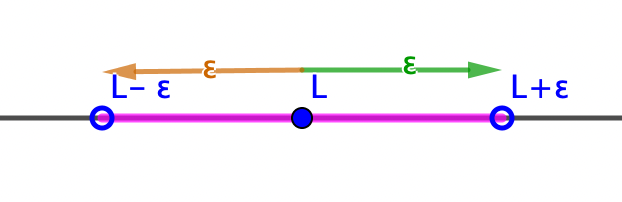
\includegraphics[scale=.5]{ws8p1.png}
\end{framed}

\item Describe $\{ x \in \R \ :  \ |3x+7|<4 \}$ explicitly in interval notation.

\begin{framed}
Since $|3x+7| = |3| |x+ \frac{7}{3}| = 3 |x+\frac{7}{3}|$, we have $|3x+7|<4$ if and only if $|x+\frac{7}{3}|< \frac{4}{3}$, so our interval goes from $\frac{-7}{3} - \frac{4}{3} = \frac{-11}{3}$ to $\frac{-7}{3} + \frac{4}{3} = -1$. That is
$(\frac{-11}{3}, -1)$.
\end{framed}

\item Suppose that $|x-2|< \frac{1}{5}$, $|y-2|< \frac{2}{5}$.

\begin{enumerate}
\item Show that $x > \frac{8}{5}$.
\item Show that $|x-y| < \frac{3}{5}$.
\item Use the reverse triangle inequality to show that $|y-3|>\frac{3}{5}$.
\end{enumerate}

\begin{framed}
\begin{enumerate}
\item Since $|x-2|<\frac{1}{5}$, we have $-(x-2) \leq |x-2|<\frac{1}{5}$, so $x-2 > -\frac{1}{5}$, and $x > 2-\frac{1}{5} = \frac{9}{5}> \frac{8}{5}$.
\item By the triangle inequality, $|x-2|<  \frac{1}{5}$ and $|y-2|<  \frac{2}{5}$ implies $|x-y| <  \frac{1}{5} + \frac{2}{5} = \frac{3}{5}$.
\item Applying the reverse triangle inequality with $y$, $2$, and $3$, we have $|y-3| \geq ||3-2| - |y-2|| = |1 - |y-2||$. Since $|y-2|<\frac{2}{5}$, $1-|y-2| > 0$, so $|1 - |y-2|| = 1- |y-2| > 1- \frac{2}{5} = \frac{3}{5}$.
\end{enumerate}

\end{framed}

\item True or false \& justify$^{\text{1}}$: There is a rational number $x$ such that $|x^2 - 2| = 0$.

\begin{framed}
False! This would imply that $x^2=2$, and there is no such rational number.
\end{framed}

\item True or false \& justify\footnote{You can use anything we've proven in class, but don't use things we haven't, like decimal expansions.}: There is a rational number $x$ such that $|x^2 - 2| < \frac{1}{1000000}$.

\begin{framed}
True! There is a rational number $x$ in the interval $(\sqrt{2} - \frac{1}{4000000}, \sqrt{2} + \frac{1}{4000000})$ by density of rational numbers. In particular, $x < \sqrt{2} +  \frac{1}{4000000} < 2$ so $|x+ \sqrt{2}| < 2 + 2 = 4$. (This is a crude bound, but good enough.)
Then $|x^2-2| = |x-\sqrt{2}| \cdot |x+\sqrt{2}| < \frac{1}{4000000} \cdot 4 = \frac{1}{1000000}$.
\end{framed}



\end{enumerate}



\begin{framed}
\noindent Here is another important fact in the relationship between $\R$ and $\Z$:

\

\noindent \textsc{Theorem 8.3:} For every real number $r$, there is a unique integer $n\in \Z$ such that $n\leq r < n+1$.
\end{framed}

\begin{enumerate}\setcounter{enumi}{6}
\item Proof of Theorem 8.3:
\begin{enumerate}
\item First, assume that $r\geq 0$. Complete the following sentence:
``The number  $n+1$ \ should be the smallest natural number that \underline{\phantom{bananananananana}}.''
\begin{framed} is larger than $r$.\end{framed}
\item Take your sentence and turn it into a recipe for $n$ to prove that such an integer $n$ exists in this case.
\begin{framed} Assume that $r\geq 0$. Consider the set $S=\{ m\in \N \ | \ m> r\}$. By Theorem 7.1, $S$ is nonempty, so by the Well-Ordering Axiom for $\N$, there is a minimum element in $S$. Set $n=\min(S)-1$; note that $r<n+1$ because $n+1\in S$. If $\min(S)>1$, $n\in \N \smallsetminus S$, since $n$ is less than the minimum for $S$, so $n\leq r$.  If $\min(S)=1$, then $n=0$, so by our assumption, $n=0\leq r$.
Either way, $n\in \N\cup \{0\} \subseteq \Z$ and $n\leq r \leq n+1$, as required.
\end{framed}
\item Now, assume that $r<0$. Explain why there is some $j\in \N$ such that $j+r >0$. Deduce that an integer $n$ as in the statement exists in this case too.
\begin{framed}
Now assume that $r<0$. By Theorem~7.1, there is some $j\in \N$ such that $j>-r$, so $j+r>0$. By the case we already established, there is some integer $n\in \Z$ such that $n \leq j+r < n+1$. We then have $n-j \leq r < (n-j)+1$, so $n-j\in \Z$ is the integer we seek.
\end{framed}
\item Finally, prove that $n$ is unique. You can use without proof that there are no integers in between $0$ and $1$.
\begin{framed} To see that $n$ is unique, suppose that $n,m\in \Z$ with $n\leq r < n+1$ and $m\leq r < m+1$. We then have $n < m+1$, so $n\leq m$, and, switching roles, $m\leq n$. Thus, $m=n$.
\end{framed}
\end{enumerate}
\end{enumerate}

\newpage


\Sept{16}{\Mo}{2.1}




We now turn our attention to the next major topic of this class: sequences of real numbers. We will spend the next few weeks developing their properties carefully and
rigorously. Sequences form the foundation for much of what we will cover for the rest of the semester. 


\begin{defn} A {\bf sequence}\index{sequence} is an infinite list of real numbers indexed by $\N$:
$$
a_1, a_2, a_3, \dots.
$$
(Equivalently, a sequence is a function from $\N$ to $\R$: the value of the function at $n \in \N$ is written as $a_n$.)

We will usually write $\{a_n\}_{n=1}^\infty$ for a sequence.
\end{defn}

\begin{ex} To describe sequences, we will typically give a formula for the $n$-th term, $a_n$, either an explicit one or a recursive one. On rare occasion we'll
  just list enough terms to make the pattern clear. Here are some examples:
\begin{enumerate}

\item $\{5 + (-1)^n \frac{1}{n}\}_{n=1}^\infty$ is the sequence that starts
$$
4, \frac{11}2,  \frac{14}{3}, \frac{21}4, \frac{24}5, \dots.
$$

\item Let $\{a_n\}_{n=1}^\infty$ be defined by $a_1 = 1, a_2 = 1$ and $a_n = a_{n-1} + a_{n-2}$ for all $n \geq 2$. This gives the sequence
$$
1, 1, 2, 3, 5, 8, 13, 21, 34, \dots
$$
This is an example of a recursively defined sequence. It is the famed {\bf Fibonacci sequence}.\index{Fibonacci sequence} 

\item Let $\{c_n\}_{n=1}^\infty$ be the sequence whose $n$-th term is the $n$-th smallest positive prime integer:
$$
2, 3, 5, 7, 11, 13, 17, 19, 23, \dots.
$$
Note that here I have not really given an explicit formula for the terms of the sequence, but it is possible to describe an algorithm that lists every term of the sequence in
order.
\end{enumerate}

\end{ex}


You have all probably seen an ``intuitive'' definition of the limit of a sequence before. For example, you probably believe that
$$
5 + (-1)^n \frac{1}{n}
$$
converges to $5$.
Let's give the rigorous definition.

\begin{defn} Let $\{a_n\}_{n=1}^\infty$ be an arbitrary sequence and $L$ a real number. We say $\{a_n\}_{n=1}^\infty$ {\bf converges}\index{converges} to $L$ provided the
  following condition is met:
\begin{quote}
For every real number $\e > 0$, there is a real number $N$ such that ${|a_n - L| < \e}$ for all natural numbers $n$ such that $n > N$.
\end{quote}
\end{defn}

This is an extremely important definition for this class. Learn it by heart!





In symbols, the definition is 
\begin{quote}
A sequence $\{a_n\}_{n=1}^\infty$ converges to $L$ provided\\
$\forall \e >0, {\exists N \in \R} : {\forall n \in \N} \text{ s.t. } n > N, \ {|a_n - L| < \e}$. 
\end{quote}

It's a complicated definition --- three quantifiers!


Here is what the definition is saying somewhat loosely: No matter how small a number $\e$ you pick, so long as it is positive, if you go far enough out in the sequence, all of
the terms from that point on will be within a distance of $\e$ of the limiting value~$L$.

\begin{ex} To say that the sequence $\{a_n\}_{n=1}^\infty$ where $a_n =  5 + (-1)^n \frac{1}{n}$ converges to $5$ gives us a different statement for every $\e>0$. For example:
\begin{itemize}
\item Setting $\e=3$, there is a number $N$ such that for every natural number $n>N$, $|a_n-5|<3$. Namely, we can take $N=0$, since for \emph{every} term $a_n$ of the sequence, $|a_n-5|<3$ holds true.
\item Setting $\e=\frac13$, there is a number $N$ such that for every natural number $n>N$, $|a_n-5|<\frac13$. We cannot take $N=0$ anymore, since $1>0$ and $|a_1-5|=1>\frac13$. However, we can take $N=3$, since for $n>3$, $|a_n-5|=\frac1n <\frac13$.
\item Setting $\e=1/1000000$, there is a number $N$ such that for every natural number $n>N$, $|a_n-5|<1/1000000$. We need a bigger $N$; now $N=1000000$ works.
\end{itemize}

In general, our choice of $N$ may depend on $\e$, which is OK since our definition is of the form $\forall \e>0,\exists N\dots$ rather than $\exists N:\forall \e>0\dots$.
\end{ex}



\begin{ex} I claim the sequence $\{a_n\}_{n=1}^\infty$ where $a_n =  5 + (-1)^n \frac{1}{n}$ converges to $5$. I'll give a rigorous proof, along with some commentary and
  ``scratch work'' within the parentheses. 

\begin{proof} Let $\e > 0$ be given. 

(Scratch work: Given this $\e$, our goal is to find $N$ so that if $n > N$, then 
$|5 + (-1)^n \frac{1}{n} - 5| < \e$. The latter simplifies to
$\frac{1}{n} < \e$, which in turn is equivalent to $\frac{1}{\e} < n$ since
$\e$ and $n$ are both positive.  So, it seems we've found the $N$ that
``works''. Back to the formal proof....)


Let $N = \frac{1}{\e}$. Then $\frac{1}{N}
= \e$, since $\e$ is positive.  

(Comment: We next show that this is the $N$ that ``works'' in
the definition. Since this involves proving something about every natural number that is bigger than $N$, 
we start by picking one.) 

Pick any $n \in \N$ such that  $n >
N$. Then $\frac{1}{n} < \frac{1}{N}$ and hence
$$
|a_n - 5| = |5 + (-1)^n \frac{1}{n} - 5| = 
|(-1)^n \frac{1}{n}| = \frac{1}{n} < \frac{1}{N} = \e.
$$
This proves that 
$\{5 + (-1)^n \frac{1}{n}\}_{n=1}^\infty$ converges to $5$.
\end{proof}
\end{ex}


\begin{rem} A direct proof that a certain sequence converges to a certain number follows the general outline:
\begin{itemize}
	\item Let $\e > 0$ be given. (or, if your prefer, ``Pick $\e > 0$.")
	\item Let $N =$ [expression in terms of $\e$ from scratch work].
	\item Let $n \in \N$ be such that $n > N$.
\item $\text{[Argument that $|a_n-L|<\e$.]}$
	\item Thus $\{a_n\}_{n=1}^{\infty}$ converges to $L$.
\end{itemize}

In particular, you usually can't just sit down and write a proof in one fell swoop: you will have to preapre for your proof by figuring out what value of $N$ will beat $\e$. The work that you use to find $N$ in terms of $\e$ does \emph{not} belong in the final proof.
\end{rem}



\begin{ex} I claim that the sequence
$$
\left\{ \frac{2n - 1}{5n + 1} \right\}_{n=1}^\infty
$$
converges to $\frac{2}{5}$.  Again I'll give a proof with commentary and scratch work in parentheses.

\begin{proof} 
Let $\e > 0$ be given. 

(Scratch work: We need $n$ to be large enough so that
$$
\left|\frac{2n - 1}{5n + 1} - \frac{2}{5}\right| < \e.
$$
This simplifies to 
$\left|\frac{-7}{25n + 5}\right| < \e$
and thus to
$\frac{7}{25n + 5} < \e$, which we can rewritten as $\frac{7}{25\e} - \frac15 < n$.)

Let $N = \frac{7}{25\e} - \frac15$. We solve this equation for $\e$: We get
$\frac{7}{25 \e} = \frac{5N +  1}{5}$ and hence 
$\frac{25 \e}{7} = \frac{5}{5N +  1}$, which gives finally
$$
\e = \frac{7}{25N + 5}.
$$

(Next we show this value of $N$ works....)

Now pick any $n \in \N$ is such that
$n > N$. Then
$$
\left|\frac{2n - 1}{5n + 1} - \frac{2}{5}\right| 
= \left|\frac{10n - 5   - 10n -2               }{25n + 5} \right| 
=  \frac{7}{25n + 5}.
$$
Since $n > N$, $25n + 5> 25N + 5$ and hence
$$
\frac{7}{25n + 5} < \frac{7}{25N + 5} = \e.
$$
We have proven that if $n \in \N$ and $n > N$, then
$$
\left|\frac{2n - 1}{5n + 1} - \frac{2}{5}\right| < \e.
$$
This proves $\left\{ \frac{2n - 1}{5n + 1} \right\}_{n=1}^\infty$
converges to $\frac25$.
\end{proof}
\end{ex}

\newpage
\Sept{18}{\We}{2.1}


\begin{framed}
\noindent \textsc{Definition:} A sequence $\{a_n\}_{n=1}^\infty$ {\bf converges} to a real number $L$ provided for every real number $\e > 0$, there is a real number $N$ such that ${|a_n - L| < \e}$ for all natural numbers $n$ such that $n > N$.
\end{framed}
\begin{enumerate}
\item \textsc{The $\e$ vs $N$ game:}
\begin{enumerate}
\item Player 0 starts by graphing a sequence $\{a_n\}_{n=1}^\infty$, and specifies $y$-value $L$ that  they think makes $\lim_{n\to \infty} a_n = L$ \textit{true}. [You can't graph all the values, but make a large graph with a generous number of values.]
\item Player 1 choses an $\e$. This is how close we would like our sequence to be to $L$. Thus, $\e$ goes up and down from $L$ (corresponding to $|a_n-L|<\e$). Draw horizontal dotted lines with $y$-values $L-\e$ and $L+\e$. [The $\e$ should be large enough for people to see and have room to work in the picture.]
\item Player 2 must find an $N$ such that all of the values of the sequence to the right of $N$ are in $(L-\e,L+\e)$.
Draw a vertical line for $x=N$.
[Everyone in the team can assist player 2!]
\item Repeat with the same graph, players 1\& 2 switching roles (and a new $\e$).
\item Now do a couple of rounds with a sequence $\{a_n\}_{n=1}^\infty$ and an $L$ that you think makes $\lim_{n\to \infty} a_n = L$ \textit{false}.
\end{enumerate}

\

\item Prove that the sequence $\ds \left\{ \frac{1}{\sqrt{n}} \right\}_{n=1}^\infty$ converges to $0$.

\


\item Let $\ds \{a_n\}_{n=1}^\infty$ be a sequence. Suppose we know that $\{a_n\}_{n=1}^\infty$ converges to $1$. Prove\footnote{Hint: If you know that a ``for all'' statement is true, you can choose any specific value for that variable and get a more specific true statement.} that there is a natural number $n\in \N$ such that $a_n>0$.

\begin{framed}
Take $\e = 1$. By definition of converges to $1$, there is some $N$ such that for all $n>N$, $|a_n  - 1|< 1$, and in particular $a_n >0$. So, take any natural number greater than $n$, and the conclusion follows.
\end{framed}



\item Prove or disprove: The sequence $\ds \left\{\frac{n+1}{2n} \right\}_{n=1}^\infty$ converges to $0$.

\begin{framed}
Take $\e = 1/2$. We claim that there is no $N$ such that for all $n>N$ we have $|a_n - 0| < 1/2$. Indeed, given $N$, take any $n$ to be any natural number greater than $N$. Then $a_n = 1/2 + 1/2n > 1/2$, so $|a_n| > 1/2$. Thus, there is no $N$ satisfying the desired property. This means that the sequence does not converge to $1/2$.
\end{framed}


\end{enumerate}

\newpage

\begin{comment}

\Sept{23}{Mo}{2.1}

\begin{defn} We say that a sequence $\{ a_n \}_{n=1}^\infty$ is \textbf{convergent} if there is a number $L$  such that $\{ a_n \}_{n=1}^\infty$ converges to $L$, and \textbf{divergent} otherwise.
\end{defn}


\begin{ex} Let's prove the sequence $\{(-1)^n\}_{n=1}^\infty$ is divergent.

\begin{proof}
  We proceed by contradiction: Suppose the sequence did converge to some number $L$. Our strategy will be to derive a contradiction by showing that such
  an $L$ would have to satisfy mutually exclusive conditions. 

By definition, since the sequence converges to $L$, we have that 
for every $\e > 0$ there is a number $N$ such that 
$|(-1)^n - L| < \e$
for all natural numbers $n$ such that $n > N$.
In particular, this statement is true for the particular value $\e = \frac12$. That is,  there is a number $N$ such that  
$|(-1)^n - L| < \frac12$ for all natural numbers $n$ such that  
$n > N$. Let $n$ be any even natural number that is bigger than
$N$. (Certainly one exists: we know there is an integer bigger than
$N$
by Theorem \ref{thm120}. Pick one. If it is even, take that to be
$n$. If it is odd, increase it by one to get an even integer $n$.)  Since $(-1)^n = 1$ for an even integer $n$, we get
$$
|1 - L| < \frac12
$$
and thus $\frac12 < L < \frac32$.

Likewise, let $n$ be an odd natural number bigger than $N$. Since $(-1)^n = -1$ for an odd integer $n$, we get
$$
|-1 - L| < \frac12
$$
and thus $-\frac32 < L < -\frac12$. But it cannot be that both $L > \frac12$ and $L < -\frac12$.

We conclude that no such $L$ exists; that is, this sequence is divergent.
\end{proof}
\end{ex}

%\Sept{17}


\begin{prop} If a sequence converges, then there is a unique number to which it converges.
\end{prop}



\begin{proof} Recall that to show something satisfying certain properties is unique, one assumes there are two such things and argues that they must be equal. 
So,
suppose $\{a_n\}_{n=1}^\infty$ is a sequence that converges to $L$ and that also converges to $M$. We will prove $L = M$. 

By way of contradiction, suppose $L \ne M$. Then set $\e =
\frac{|L-M|}{3}$. Since we are assuming $L \ne M$, we have $\e > 0$.  
According to the definition of convergence, since the sequence converges to $L$, there is a real number $N_1$ such that for $n \in \N$ such that  $n > N_1$ we have
$$
|a_n - L| < \e.
$$

Also according to the definition, since the sequence converges to $M$, there is a real number $N_2$ such that for $n \in \N$ and  $n > N_2$ we have
$$
|a_n - M| < \e.
$$
Pick $n$ to be any natural number larger than $\max\{N_1, N_2\}$ (which exists by Theorem \ref{thm120}).   For such an $n$, both
$|a_n - L| < \e$ and $ |a_n - M| < \e$ hold. 
Using the triangle inequality and these two inequalities, we get
$$
|L-M| \leq |L-a_n| + |M-a_n| < \e + \e.
$$
But by the choice of $\e$, we have $\e + \e = \frac23 |L-M|$. That is, we have deduced that $|L-M| < \frac23 |L-M|$ which is impossible.
We conclude that $L = M$. 
\end{proof}




From now on, given a sequence $\{a_n\}_{n=1}^\infty$ and a real number $L$, 
will we use the short-hand notation\index{$\lim_{n\to\infty} a_n$}
$$
\lim_{n \to \infty} a_n = L
$$
to mean that the given sequence converges to the given number. For example, we showed above that 
$$
\lim_{n \to \infty} \frac{2n - 1}{5n + 1}   = \frac25.
$$
But, to be clear, the statement ``$\lim_{n \to \infty} a_n = L$''
signifies nothing more and nothing less than the statement
``$\{a_n\}_{n=1}^\infty$ converges to $L$''.



Here is some terminology we will need:

\begin{defn} Suppose $\{a_n\}_{n=1}^\infty$ is any sequence. 

\begin{enumerate}

\item 
We say $\{a_n\}_{n=1}^\infty$ is {\em bounded above}\index{bounded above} if there  exists at least one real number $M$ such that $a_n \leq M$ for all $n   \in
\N$; 
we say $\{a_n\}_{n=1}^\infty$ is {\em bounded below}\index{bounded below} if there  exists at least one real number $m$ such that $a_n \geq m$ for all $n   \in
\N$; and we say 
$\{a_n\}_{n=1}^\infty$ is {\em bounded}\index{bounded} if it is both bounded above and bounded below.

\item We say $\{a_n\}_{n=1}^\infty$ is {\em increasing}\index{increasing} if for all $n \in \N$, $a_n \leq a_{n+1}$;
we say $\{a_n\}_{n=1}^\infty$ is {\em decreasing}\index{decreasing} if for all $n \in \N$, $a_n \geq a_{n+1}$; and we say
$\{a_n\}_{n=1}^\infty$ is {\em monotone}\index{monotone} if it is either decreasing or increasing.

\item We say $\{a_n\}_{n=1}^\infty$ is {\em strictly increasing}\index{strictly increasing} if for all $n \in \N$, $a_n < a_{n+1}$. I leave the definition of
{\em strictly decreasing}\index{strictly decreasing} and {\em strictly monotone}\index{strictly monotone} to your imaginations.
\end{enumerate}
\end{defn}


\begin{rem} Be sure to interpret ``monotone'' correctly. It means
$$
\left(\forall n \in \N, a_n \leq a_{n+1}\right) \text{ or }
\left(\forall n \in \N, a_n \geq a_{n+1}\right);
$$
it does {\em not} mean
$$
\forall n \in \N, \left( a_n \leq a_{n+1}\right) \text{ or } \left(a_n \geq a_{n+1}\right).
$$
Do you see the difference?
\end{rem}




\begin{prop} \label{prop21}
	If a sequence $\{a_n\}_{n=1}^\infty$ converges then it is bounded.
\end{prop}

\begin{proof} Suppose the sequence $\{a_n\}_{n=1}^\infty$ converges to
	the number $L$. Applying the definition of ``converges to $L$'' using the particular value $\e = 1$ gives the following fact:
	There is a real number $N$ such that if $n \in \N$ and $n > N$, then $|a_n -
	L| < 1$. The latter inequality is equivalent to  $L-1 < a_n < L+1$
	for all $n > N$.
	
	Let $m$ be any natural number such that $m > N$,
	and consider the finite list of numbers
	$$
	a_1, a_2, \dots, a_{m-1}, L + 1.
	$$
	Let $b$ be the largest element of this list. I claim the sequence is bounded above by $b$.
	For any $n \in  \N$, if $1 \leq n \leq m-1$, then $a_n \leq b$ since in this case $a_n$ is a member of the above list and $b$ is the largest element of this list.
	If $n \geq m$ then since $m > N$, we have $n > N$ and hence $a_n < L + 1$ from above. We also have $L + 1 \leq b$ (since $L+1$ is in the list) and thus $a_n < b$. 
	This proves $a_n \leq b$ for all $n$ as claimed.
	
	Now take $p$ to be the smallest number in the list
	$$
	a_1, a_2, \dots, a_{m-1}, L - 1.
	$$
	A similar argument shows that $a_n \geq p$ for all $n \in \N$.
\end{proof}

\Sept{22}

\begin{enumerate}

\item For each of the following sequences which of the following adjectives apply: bounded above, bounded below, bounded, (strictly) increasing, (strictly) decreasing, (strictly) monotone?
\begin{enumerate}
\item $\{ \frac{1}{n} \}_{n=1}^\infty$
\item The Fibonacci sequence $\{ f_n \}_{n=1}^\infty$ where $f_1=f_2=1$ and $f_n= f_{n-1} + f_{n-2}$ for $n\geq 3$.
\item $\{(-1)^n \}_{n=1}^\infty$
\item $\{ 5 + (-1)^n \frac{1}{n}  \}_{n=1}^\infty$.
\end{enumerate}

\begin{framed}
\begin{enumerate}
\item bounded, strictly decreasing, strictly monotone
\item bounded below, increasing, monotone
\item bounded
\item bounded
\end{enumerate}
\end{framed}

\item Prove or disprove the converse to Proposition~9.5.
\begin{framed}
The sequence $\{(-1)^n\}_{n=1}^\infty$ is bounded but divergent, so the converse is false.
\end{framed}
\end{enumerate}


\begin{ex}
\begin{enumerate}
\item A constant sequence $\{c\}_{n=1}^\infty$ converges to $c$.
\item The sequence $\{\frac{1}{n}\}_{n=1}^\infty$ converges to $0$.
\end{enumerate}
\end{ex}


\begin{thm}[Limits and algebra]\label{thm99}
Let $\{a_n\}_{n=1}^\infty$ be a sequence that converges to $L$, and $\{b_n\}_{n=1}^\infty$ be a sequence that converges to $M$.
\begin{enumerate}
\item If $c$ is any real number, then $\{ c a_n\}_{n=1}^\infty$ converges to $cL$.
\item The sequence $\{a_n + b_n\}_{n=1}^\infty$ converges to $L+M$.
\item The sequence $\{a_n b_n\}_{n=1}^\infty$ converges to $LM$.
\item If $L\neq 0$ and $a_n\neq 0$ for all $n\in \N$, then $\displaystyle\left\{\frac{1}{a_n}\right\}_{n=1}^\infty$\!\!\! converges to~$\displaystyle \frac{1}{L}$.
\item If $M\neq 0$ and $b_n\neq 0$ for all $n\in \N$, then $\displaystyle\left\{\frac{a_n}{b_n}\right\}_{n=1}^\infty$\!\!\! converges to~$\displaystyle \frac{L}{M}$.
\end{enumerate}
\end{thm}
(end of theorem, back to problems)

\begin{enumerate}\setcounter{enumi}{2}

\item Use Theorem~10.2 and Example~10.1 to show that the sequence $\{2 + 5/n - 7/n^2\}_{n=1}^\infty$ converges to $2$.

\begin{framed}
The constant sequence $\{2\}_{n=1}^\infty$ converges to $2$ by Ex 10.1 part 1. The sequence $\{5/n\}_{n=1}^\infty = \{5 \cdot 1/n\}_{n=1}^\infty$ converges to $5\cdot 0 = 0$ by Ex 10.1 part 2 and Thm 10.2 part 1. The sequence $\{ -7/n^2\}_{n=1}^\infty = \{ -7 \cdot 1/n \cdot 1/n\}_{n=1}^\infty$ converges to $-7 \cdot 0 \cdot 0 = 0$ by Ex 10.1 part 2, Thm 10.2 part 1, and Thm 10.2 part 3. Thus, by Thm 10.2 part 2, the sequence $\{ 2 + 5/n - 7/n^2\}_{n=1}^\infty$ converges to $2+0+0 = 2$ by Thm 10.2 part 2.
\end{framed}

\item Use Theorem~10.2 and Example~10.1 to show that the sequence $\frac{2n+3}{3n-4}$ converges to $\frac23$.

\

\item Use Theorem~10.2 to show that if $\{a_n\}_{n=1}^\infty$ converges to $L$, and $\{b_n\}_{n=1}^\infty$ converges to $M$, then $\{a_n - b_n\}_{n=1}^\infty$ converges to $L-M$.

\begin{framed}
By Thm 10.2 part 1, $\{-b_n\}_{n=1}^\infty$ converges to $-M$. Then by Thm 10.2 part 2, $\{a_n - b_n\}_{n=1}^\infty = \{a_n + (- b_n)\}_{n=1}^\infty$ converges $L+(-M) = L-M$.
\end{framed}

\item Prove or disprove the following converse to part (2): If $\{ a_n + b_n \}_{n=1}^\infty$ converges to $L+M$ then $\{a_n \}_{n=1}^\infty$ converges to $L$ and $\{ b_n \}_{n=1}^\infty$ converges to $M$.

\begin{framed}
Take $\{ a_n\}_{n=1}^\infty = \{ (-1)^n\}_{n=1}^\infty$ and $\{ b_n \}_{n=1}^\infty = \{ (-1)^{n+1} \}_{n=1}^\infty$. Then $\{ a_n + b_n\}_{n=1}^\infty = \{ 0 \}_{n=1}^\infty$ converges to $0$, but neither $\{a_n\}_{n=1}^\infty$ nor $\{b_n\}_{n=1}^\infty$ converges.
\end{framed}


\item Prove part (1) of Theorem~10.2  in the special case $c=2$ by following the following steps:
\begin{itemize}
\item Assume that $\{a_n \}_{n=1}^\infty$ converges to $L$.
\item We now want to show that $\{ 2 a_n \}_{n=1}^\infty$ converges to something. We know what we have to write next!
\item Now we do some scratchwork: we want an $N$ such that for $n>N$ we have $|2 a_n - 2 L| < \e$. Factor this to get some inequality with $a_n$. How can we use our assumption to get an $N$ that ``works''?
\item Complete the proof.
\end{itemize}




\item Prove part (1) of Theorem~10.2.



\item Prove part~(2) of Theorem~10.2.



\item Prove part~(3) of Theorem 10.2.
\end{enumerate}



\Sept{27}

Last time we looked at:

\


\noindent \textbf{Theorem 10.2} (Limits and algebra)\textbf{.}
Let $\{a_n\}_{n=1}^\infty$ be a sequence that converges to $L$, and $\{b_n\}_{n=1}^\infty$ be a sequence that converges to $M$.
\begin{enumerate}
\item If $c$ is any real number, then $\{ c a_n\}_{n=1}^\infty$ converges to $cL$.
\item The sequence $\{a_n + b_n\}_{n=1}^\infty$ converges to $L+M$.
\item The sequence $\{a_n b_n\}_{n=1}^\infty$ converges to $LM$.
\item If $L\neq 0$ and $a_n\neq 0$ for all $n\in \N$, then $\displaystyle\left\{\frac{1}{a_n}\right\}_{n=1}^\infty$\!\!\! converges to~$\displaystyle \frac{1}{L}$.
\item If $M\neq 0$ and $b_n\neq 0$ for all $n\in \N$, then $\displaystyle\left\{\frac{a_n}{b_n}\right\}_{n=1}^\infty$\!\!\! converges to~$\displaystyle \frac{L}{M}$.
\end{enumerate}



The following is another useful technique:

\begin{thm}[The ``squeeze'' principle] \label{thm33}
Suppose 
$\{a_n\}_{n=1}^\infty$, $\{b_n\}_{n=1}^\infty$, and $\{c_n\}_{n=1}^\infty$ are three sequences such that 
$\{a_n\}_{n=1}^\infty$ and $\{c_n\}_{n=1}^\infty$ both converge to $L$, 
 and $a_n \leq b_n \leq c_n$ for all $n$.
Then $\{b_n\}_{n=1}^\infty$ also converges to $L$.
\end{thm}

 

\begin{proof}
Assume $\{a_n\}_{n=1}^\infty$ and  $\{c_n\}_{n=1}^\infty$ both
converge to $L$ and that  $a_n \leq b_n \leq c_n$ for all $n \in \N$. 
We need to prove $\{b_n\}_{n=1}^\infty$ converges to $L$.

Pick $\e> 0$.  Since  $\{a_n\}_{n=1}^\infty$ converges to $L$ there is a number $N_1$ such that if $n \in \N$ and $n > N_1$ then
$|a_n - L| < \e$ and hence $L- \e < a_n < L + \e$. Likewise, 
since $\{c_n\}_{n=1}^\infty$ converges to $L$ there is a number $N_2$ such that if $n \in \N$ and $n > N_2$ then
 $L- \e < c_n < L + \e$. Let 
$$
N = \max\{N_1, N_2\}.
$$
 If $n \in \N$ and $n > N$, then
$n > N_1$ and hence $L - \e < a_n$, and $n > N_2$ and hence $c_n < L + \e$, and also
$a_n \leq  b_n \leq  c_n$. Combining these facts gives that for $n \in \N$ such that $n > N$,
we have
$$
L - \e < b_n < L + \e
$$
and hence $|b_n - L| < \e$.
This proves $\{b_n\}_{n=1}^\infty$ converges to $L$. 
\end{proof}


\begin{ex} We can use the Squeeze Theorem to give a short proof that $\{ 5 + (-1)^n \frac{1}{n} \}_{n=1}^\infty$ converges to $5$. Note that Theorem \ref{thm99} alone cannot be used in this
  example. However, from Theorem~\ref{thm99}, it follows that $\{5-\frac{1}{n}\}_{n=1}^\infty$ and  $\{5+\frac{1}{n}\}_{n=1}^\infty$ both converge to $5$. Then, since \[5-\frac{1}{n} \leq  5 + (-1)^n \frac{1}{n} \leq 5+\frac{1}{n}\] for all $n$, our sequence also converges to $5$.\end{ex}






%Here is a corollary of the Squeeze Theorem that is sometimes handy.

%\begin{cor} If $\{|a_n|\}_{n=1}^\infty$ converges to $0$, then $\{ a_n\}$ converges to~$0$.
%\end{cor}
%\begin{proof}
%By Theorem~\ref{thm99}(1), $\{-|a_n|\}_{n=1}^\infty$ converges to $0$ as well. We have 
%\[ -|a_n| \leq a_n \leq |a_n|\]
%for all $n$, so by the Squeeze Theorem, $\{ a_n\}$ converges to $0$.
%\end{proof}

%\begin{cor}\begin{enumerate}
%		\item 	If  the sequence $\{a_n\}_{n=1}^\infty$ converges to $0$, then the sequence
%		$\{|a_n|\}_{n=1}^\infty$ also converges to $0$.
%		\item If $\{a_n\}_{n=1}^\infty$ converges to $0$ and $\{b_n\}_{n=1}^\infty$ is any bounded sequence, then $\{a_n b_n\}_{n=1}^\infty$ converges to $0$.
%	\end{enumerate}
%\end{cor}
%\begin{proof} 
%	\begin{enumerate}
%		\item Assume $\{a_n\}_{n=1}^\infty$ converges to $0$.  We need to prove $\{|a_n|\}_{n=1}^\infty$ converges to $0$. 
%		Pick $\e > 0$. Since 
%		$\{a_n\}_{n=1}^\infty$ converges to $0$, there is a number $N$ such that if $n \in \N$ and $n > N$, then $|a_n - 0| < \e$. For this same $N$, if $n > N$ then
%		$$
%		||a_n| - 0| = ||a_n|| = |a_n| < \e.
%		$$
%		This proves $\{|a_n|\}_{n=1}^\infty$ converges to $0$. 
%		\item Since $\{b_n\}$ is bounded, there is a positive real number $X$ such that $|b_n| \leq X$ for all $n$. Thus $0 \leq |a_n b_n| \leq X |a_n|$ holds
%		for all $n$ and hence
%		$$
%		- X |a_n| \leq a_n b_n \leq X |a_n|
%		$$
%		holds for all $n$. By the Lemma, since  $\{a_n\}_{n=1}^\infty$ converges to $0$, so does $\{|a_n|\}_{n=1}^\infty$. Using 
%		Theorem \ref{thm99}, we get that 
%		$\{X|a_n|\}_{n=1}^\infty$ and $\{-X|a_n|\}_{n=1}^\infty$ also both converge to $0$. Finally, by the Squeeze Theorem, $\{a_n b_n\}_{n=1}^\infty$ converges to $0$ too. \qedhere
%	\end{enumerate}
%\end{proof}
%
%
%\begin{rem} More generally, if $\{a_n\}_{n=1}^\infty$ converges to $L$, then the sequence
%  $\{|a_n|\}_{n=1}^\infty$ also converges to $|L|$, but I will not take
%  the time to prove this now. The converse of this statement is false
%  however. For example, consider the sequence $\{(-1)^n\}_{n=1}^\infty$.
%  The sequence $\{|(-1)^n|\}_{n=1}^\infty$ is the constant sequence $1$ and hence it converges to $1$, but the original sequence diverges.
%\end{rem}
%
%
%
%\begin{ex} This Corollary gives another way to prove $\{(-1)^n/n\}$ converges to $0$: take $b_n = (-1)^n$ and $a_n = 1/n$.
%  \end{ex}



 
When I introduced the Completeness Axiom, I mentioned that, heuristically, it is what tells us that the real number line doesn't have any
holes. The next result makes this a bit more precise:

\begin{thm}\label{thm226}
Every increasing, bounded above sequence converges.
\end{thm}

\begin{proof} Let $\{a_n\}_{n=1}^\infty$ be any sequence that is both  bounded above and increasing.

(Commentary: In order to prove it converges, we need to find a candidate number $L$ that
  it converges to. Since the set of numbers occurring in this sequence is nonempty and bounded above, this number is provided to us by the Completeness Axiom.) 

Let $S$ be the set of those real numbers that occur in this sequence. (This is technically different that the sequence itself, since sequences are allowed to
have repetitions but sets are not. Also, sequences have an ordering to
them, but sets do not.) 
The set $S$ is clearly
  nonempty, and it is bounded above since we assume the sequence is bounded above. Therefore, by the Completeness Axiom, $S$ has a supremum $L$. We will prove the
  sequence converges to $L$.

Pick $\e > 0$. Then $L - \e < L$ and, since $L$ is the supremum, $L - \e$ is not an upper bound of $S$. This means that 
there is an element of $S$ that is strictly bigger than $L- \e$. Every element of $S$ is a member of the sequence, and so we get that there is an $N \in \N$ such that $a_N > L - \e$. 

(We will next show that this is the $N$ that ``works''. Note that, in the general definition of convergence of a sequence, $N$ can be any real number, but in this proof it turns
out to be a natural number.)

Let $n$ be any natural number such that $n > N$. Since the sequence is increasing, $a_N \leq a_n$ and hence
$$
L - \e < a_N \leq a_n.
$$
Also, $a_n \leq L$ since $L$ is an upper bound for the sequence, and thus we have
$$
L- \e < a_n \leq L.
$$
It follows that  $|a_n - L| < \e$. We have proven the sequence converges to~$L$.
\end{proof}

%\begin{rem} Note that any increasing sequence is bounded below, for example, by its first term. Thus, an increasing sequence is bounded if and only if it is bounded below. Likewise, and decreasing sequence is bounded if and only if it is bounded above.
%\end{rem}

\begin{thm}[Monotone Converge Theorem]\label{thm:MCT}\index{monotone convergence theorem} Every bounded monotone sequence converges.
\end{thm}
\begin{proof}
If $\{a_n\}_{n=1}^\infty$ is increasing, then this is the content of Theorem~\ref{thm226}. If $\{a_n\}_{n=1}^\infty$ is decreasing and bounded, consider the sequence $\{-a_n\}_{n=1}^\infty$. If $a_n\leq M$ for all $n$, then $-a_n\geq -M$ for all $n$, so $\{-a_n\}_{n=1}^\infty$ is bounded below. Also, since $a_n \geq a_{n+1}$ for all $n$, we have $-a_n \leq -a_{n+1}$ for all $n$, so $\{-a_n\}_{n=1}^\infty$ is increasing. Thus, by Theorem~\ref{thm226}, $\{-a_n\}_{n=1}^\infty$ converges, say to $L$. Then by Theorem~\ref{thm99}(1), $\{a_n\}_{n=1}^\infty=\{-(-a_n)\}_{n=1}^\infty$ converges to $-L$.
\end{proof}

	

\begin{ex}
	Consider the sequence $\{a_n\}_{n=1}^\infty$ given by the formula
	\[ a_n = 1 + \frac{1}{2^2} + \frac{1}{3^2} + \cdots + \frac{1}{n^2}.\]
	We will use the Monotone Convergence Theorem to prove that this sequence converges.
	
	First, we need to see that the sequence is increasing. Indeed, for every $n$ we have that $a_{n+1} = a_n + \frac{1}{a_{n+1}^2} \geq a_n$.
	
	Next, we need to show that it is bounded above. Observe that
	\begin{align*} 
a_n &= 1 + \frac{1}{2^2} + \frac{1}{3^2} + \cdots + \frac{1}{n^2} \\
&\leq 1 + \frac{1}{1 \cdot 2} + \frac{1}{2 \cdot 3} + \cdots + \frac{1}{(n-1) n}\\
&= 1+ (\frac{1}{1} - \frac{1}{2}) + (\frac{1}{2} - \frac{1}{3})
 + \cdots +  (\frac{1}{n-1} - \frac{1}{n})\\
 &= 1 + 1 - \frac{1}{n},
		\end{align*}
		so we have $a_n \leq 2$ for all $n$. This means that $\{a_n\}_{n=1}^\infty$ is bounded above by $2$. 
		
		Hence, by the Monotone Convergence Theorem, $\{a_n\}_{n=1}^\infty$ converges. Leonhard Euler was particularly interested in this sequence, and was able to prove that it converges to $\frac{\pi^2}{6}$. This requires some other ideas, so we won't do that here.
	\end{ex}

\Sept{29}

\noindent Which of the following implications about sequences hold in general? Either mention a relevant theorem or give a counterexample.
	
\begin{multicols}{2}
\begin{enumerate}[label=(\alph*)]
\item monotone \ $\Longrightarrow$ \ convergent
\item convergent \ $\Longrightarrow$ \ bounded
\item bounded \ + \ decreasing  \ $\Longrightarrow$ \ convergent
\item increasing \ + \ convergent  \ $\Longrightarrow$ \ bounded
\item convergent  \ $\Longrightarrow$ \ monotone
\item bounded \ $\Longrightarrow$ \ convergent
\end{enumerate}
\end{multicols}

\begin{framed}
\begin{enumerate}[label=(\alph*)]
\item False: $\{ n\}_{n=1}^\infty$
\item True: (Every convergent sequence is bounded.)
\item True: Monotone Convergence Theorem
\item True: (Every convergent sequence is bounded.)
\item False: $\{ \frac{(-1)^n}{n}\}_{n=1}^\infty$
\item False: $\{ {(-1)^n}\}_{n=1}^\infty$
\end{enumerate}
\end{framed}


	
\noindent It is sometimes useful to distinguish between sequences like $\{(-1)^n\}_{n=1}^\infty$
that diverge because they ``oscillate'', and sequences like $
\{n\}_{n=1}^\infty$
that diverge because they ``head toward infinity''.




\begin{enumerate}[label=(\Roman*)]

\item In intuitive language, a sequence converges to $L$ if no matter how close we want or sequence to be to $L$, all values past some point are at least that close. Intuitively, a sequence \emph{diverges to $+\infty$} if no matter how large we want our sequence to be, all values past some point are at least that large. Write a precise definition for a sequence to diverge to $+\infty$.



\item Write a precise definition for a sequence to diverge to $-\infty$.
\end{enumerate} 

\begin{framed}
\begin{enumerate}[label=(\Roman*)]
\item A sequence $\{a_n\}_{n=1}^\infty$ \emph{diverges to $+\infty$}\index{diverges to $+\infty$} if for every $M\in \R$, there is some $N\in \R$ such that for every natural number $n>N$, we have $a_n >M$.
\item A sequence $\{a_n\}_{n=1}^\infty$ \emph{diverges to $-\infty$}\index{diverges to $-\infty$} if for every $m\in \R$, there is some $N\in \R$ such that for every natural number $n>N$, we have $a_n < m$.
\end{enumerate} 
\end{framed}



\begin{enumerate}

\item Carefully write the logical negation of ``$\{ a_n\}_{n=1}^\infty$ diverges to $+\infty$'' in simplified form.

\begin{framed}
There exists $M\in \R$ such that for every $N\in \R$, there exists a natural number $n>N$ with $a_n <M$.
\end{framed}

\item Use the definition to prove that the sequence $\{ \sqrt{n} \}_{n=1}^\infty$ diverges to $+\infty$.

\begin{framed}
Let $M\in \R$. [Scratchwork: We need some $N$ such that if $n>N$ then $\sqrt{n} > M$. This inequality is equivalent to $n > M^2$, so take $N=M^2$.]
Take $N=M^2$. Let $n>N$ be a natural number. Then $\sqrt{n} > \sqrt{N} = \sqrt{M^2} = |M| \geq M$. This shows that $\{ \sqrt{n} \}_{n=1}^\infty$ diverges to $+\infty$.
\end{framed}

%\item Use the definition to prove that the sequence $\{ (-1)^n\}_{n=1}^\infty$ does not diverge to $+ \infty$.

%\

\item\label{nba} Prove that if a sequence $\{ a_n\}_{n=1}^\infty$ diverges to $+\infty$ then it is not bounded above. 


\begin{framed} We prove the contrapositive. Suppose that $\{ a_n\}_{n=1}^\infty$ is bounded above, say by $M$. Suppose, to obtain a contradiction that $\{ a_n\}_{n=1}^\infty$ diverges to $+\infty$. Then applying the definition with the number $M$, we have that there is some $N$ such that for all $n>N$, $a_n>M$. But htere is no $n$ for which $a_n>M$, so this is a contradiction, so $\{ a_n\}_{n=1}^\infty$ does not diverge to $+\infty$.
\end{framed}

\item Use (\ref{nba}) to show that if a sequence diverges to $+\infty$ then it diverges.

\begin{framed}  Since every converges sequence is bounded, the conclusion follows.
\end{framed}


\item Prove or disprove: If a sequence is not bounded above, then it diverges to $+\infty$.

\begin{framed}  A counterexample is given by the sequence $\{ (-1)^n n \}_{n=1}^\infty$. It is not bounded above, since for any $M$, we can take an even natural number $n$ larger than $M$, and for this number, $(-1)^n  n = n >M$. It does not diverge to $+\infty$: take $M=0$; for any $N\in \R$, there is an odd natural number $n$ larger than $N$, and for this $n$, we have $(-1)^n n = - n < 0 = M$.
\end{framed}

\item Prove or disprove:  If a sequence diverges to $+\infty$ then it is increasing.

\begin{framed}  A counterexample is given by the sequence given by $a_1 = 3$, $a_n=n$ for $n>1$. It is not increasing since $a_1=3 > 2 = a_2$. However, it diverges to $+\infty$ since, given $M$, we can take $N=M$, and for any $n>N$, we have $a_n=n>N=M$.
\end{framed}

\item Prove or disprove: If a sequence is increasing and not bounded above, it diverges to~$\infty$.

\begin{framed} 
To prove it, let $\{ a_n\}_{n=1}^\infty$ be  increasing and not bounded above. Take $M\in \R$. Since it is not bounded above, there is some $N\in \N$ such that $a_N >M$. Then, for this $N$, for any $n>N$ we have $a_n \geq a_N$ since the sequence is increasing, so $a_n > M$. This shows the sequence diverges to $+\infty$.
\end{framed}

\end{enumerate}

\Oct{4}
	
We will now embark on a bit of detour. I've postponed talking about proofs by induction, but we will need to use that technique on occasion. So let's talk
about that idea now. 

The technique of proof by induction is used to prove that an infinite sequence of statements indexed by $\N$
$$
P_1, P_2, P_3, \dots
$$
are all true. For example the equation
$$
1 + 2 + \cdots + n = \frac{n(n+1)}{2}
$$
holds for all $n \in \N$. We get one statement for each natural number:

\[\begin{array}{ccrrl}
	&P_1: &&1 &= \displaystyle\frac{1 \cdot 2}{2}\\[10pt]
		&P_2: &&1 + 2 &=\displaystyle\frac{2 \cdot 3}{2}\\[10pt]
		&P_3: &&1 +2 + 3 &=\displaystyle\frac{3 \cdot 4}{2}\\[10pt]
		&\vdots &&\vdots&
	\end{array}\]

Such a fact (for all $n$) is well-suited to be proven by induction.

Here is the general principle:

\begin{thm}[Principle of Mathematical Induction]\index{induction} Suppose we are given, for each $n \in \N$, a statment $P_n$.  
Assume that $P_1$ is true and that for each $k
  \in \N$, if $P_k$ is true, then $P_{k+1}$ is true. Then $P_n$ is true for all $n \in \N$.
\end{thm}

``The domino analogy'': Think of the statements $P_1, P_2, \dots$ as dominoes lined up in a row. The fact that $P_k \implies P_{k+1}$ is interpreted as meaning
that the dominoes
are arranged well enough so that if one falls, then so does the next one in the line. The fact that $P_1$ is true is interpreted as meaning the first one has been knocked
over. Given these assumptions, for every $n$, the $n$-th domino will (eventually) fall down. 



The Principle of Mathematical Induction (PMI) is indeed a theorem, which we will now prove:

\begin{proof} 
Assume that $P_1$ is true and that for each $k
  \in \N$, if $P_k$ is true, then $P_{k+1}$ is true.
Consider the subset
$$
S = \{n \in \N \mid \text{ $P_n$ is false} \}
$$
of $\N$. Our goal is to show $S$ is the empty set. 

By way of contradiction, suppose $S$ is not empty. Then
by the Well-Ordering Principle, $S$ has a smallest element, call it $\ell$. (In other words, $P_\ell$ is the first statement in the list $P_1, P_2, \dots, $
that is false.) Since $P_1$ is true, we must have $\ell > 1$. But then
$\ell-1 < \ell$ and so $\ell-1$ is not in $S$. Since $\ell > 1$, we have $\ell-1 \in
\N$ and thus we can say that $P_{\ell-1}$ must be true. 
Since $P_k \Rightarrow P_{k+1}$ for any $k$,  letting $k = \ell-1$, we see that, since $P_{\ell-1}$ is true, $P_{\ell}$ must also by true. This contradicts the fact that $\ell \in S$. We
conclude that $S$ must be the empty set.
\end{proof}

The above proof shows that the Principle of Mathematical Induction is a consequence of the Well-Ordering Principle. The converse is also true.

\begin{ex}
Let's prove that the formula
\[ 1 + 2 + 3 + \cdots + n = \frac{n(n+1)}{2}\]
for every natural number $n$.
Here, $P_k$ is
\[ 1 + 2 + 3 + \cdots + k = \frac{k(k+1)}{2}.\]
For $P_1$ we have $1 = \frac{1 \cdot 2}{2}$ is true. Now we show $P_k$ implies $P_{k+1}$. Let $k$ be a natural number and assume that 
\[ 1 + 2 + 3 + \cdots + k = \frac{k(k+1)}{2}.\] Then 
\begin{align*} 1 + 2 + 3 + \cdots + k + (k+1) &= (1 + 2 + 3 + \cdots + k )+ (k+1) \\&= \frac{k(k+1)}{2} + (k+1) \\&=  \frac{k(k+1)}{2} + \frac{2(k+1)}{2} \\& = \frac{(k+1)(k+2)}{2} = \frac{(k+1)((k+1)+1)}{2},\end{align*}
which is $P_{k+1}$. Thus we have proven the equality for all natural numbers $n$ by induction.\qed
\end{ex}

\begin{ex} Let us show that for every real number $x\geq -1$, and every natural number $n\in \N$, the inequality $(1+x)^n \geq 1+nx$.

Fix a real number $x\geq -1$. We show that $(1+x)^n \geq 1+nx$ for all natural numbers $n$ by induction. For $n=1$, we have 
\[ (1+x)^1 = 1+x = 1+ 1\cdot x,\]
so the statement is true for $n=1$. Let $k$ be a natural number and assume that
\[ (1+x)^k \geq 1+kx.\]
Then,
\[ (1+x)^{k+1} = (1+x)\cdot (1+x)^k \geq (1+x) (1+kx) = 1 + (k+1) x + kx^2 \geq 1 + (k+1) x,\]
where we used that $1+x\geq 0$ in the first $\geq$ (since $x\geq -1$) and that $x^2\geq 0$ in the second $\geq$.
Thus, by induction, the inequality is true for all $n\in \N$.\qed
\end{ex}


Induction is also closely related to the notion of a sequence defined by recursion. Recall that we define a sequence $\{a_n\}_{n=1}^\infty$ recursively by specifying a value $a_1$ for the first value, and a formula for $a_n$ in terms of $a_{n-1}$ (or multiple earlier values in the sequence). The principle of induction justifies that such a rule gives a well-defined value for every $n$: if we take $P_k$ to be the statement that the formulas define value for all of the first $k$ terms $a_1,\dots,a_k$, then $P_1$ is true and $P_k \Rightarrow P_{k+1}$, so $P_n$ is true for every $n\in \N$.

\begin{prop}
For any real number $r$, there exists a strictly increasing sequence of rational numbers that converges to $r$.
\end{prop}
\begin{proof}
We will construct a sequence of rational numbers $\{q_n\}_{n=1}^\infty$ such that $r-\frac{1}{n} < q_n < r$ for every $n$ that is strictly increasing, and then show that this sequence converges to $r$. By Density of Rational Numbers, there exists a rational number $q_1$ such that $r-1 < q < r$. Given $q_1,\dots,q_n$, we define $q_{n+1}$ recursively to be a rational number such that $\max\{r-\frac{1}{n+1}, q_n\} < q_{n+1} < r$ again using Density of Rational Numbers. To see that this rule makes sense, we observe that if we have constructed $q_1,\dots ,q_n$ by this rule, then  $q_n<r$, so $\max\{r-\frac{1}{n+1}, q_n\} < r$, and hence Density of Rational number applies, so we can construct $q_{n+1}$ (and hence we can construct $q_n$ for any $n$ by this rule). Since \[ q_n \leq \max\{r-\frac{1}{n+1}, q_n\} < q_{n+1}\] for every $n$, the sequence we obtain is strictly increasing. Since \[ r-\frac{1}{n}< q_{n} < r\] for every~$n$ and $\{ r - \frac{1}{n}\}_{n=1}^\infty$ converges to $r$, by the Squeeze Theorem, the sequence $\{q_n\}_{n=1}^\infty$ converges to $r$.
\end{proof}




\Oct{6}


	
	\subsection*{Decimal expansions}
	
	In this worksheet, we are going to define decimal expansions and prove the basic properties about them. To simplify things, we are going to only deal with numbers between $0$ and $1$ (since we get all the the rest by adding integers and taking negatives). Along the way we will use induction and convergence of sequences in an important way. Before we define infinite decimal expansions, let's review finite decimal expansions. 

\begin{enumerate}

\item If $d \in \{ 0,1,\dots,9\}$ (i.e., $d$ is an integer between $0$ and $9$), what does the decimal number $0.d$ mean? Express it as a rational number.

\begin{framed}
\[\frac{d}{10}\]
\end{framed}

\item  If $d_1,d_2,\dots,d_n \in \{ 0,1,\dots,9\}$ (i.e., $d_1,\dots,d_n$ are a bunch of integers between $0$ and $9$, which may or may not have repeats), convince yourself that  the decimal number $0.d_1 d_2 \cdots d_n$ in the way that we commonly use it is shorthand for
\[ 0.d_1 d_2 \cdots d_n = \frac{d_1}{10^1} + \frac{d_2}{10^2} + \cdots + \frac{d_n}{10^n}.\]

\end{enumerate}


 Let's say that a sequence of the form $\{d_n\}_{n=1}^\infty$ is a \emph{digit sequence} if $d_n\in \{0,1,\dots, 9\}$ for all~$n$. (That is a digit sequence is just a sequence of integers between $0$ and $9$.) Given a digit sequence $\{d_n\}_{n=1}^\infty$, define another sequence $\{D_n\}_{n=1}^\infty$ by the rule
\[ \begin{aligned} D_1 &= \frac{d_1}{10^1}\\
D_2 &= \frac{d_1}{10^1} + \frac{d_2}{10^2}\\
& \ \ \vdots\\
D_n& = \frac{d_1}{10^1} + \frac{d_2}{10^2} + \cdots + \frac{d_n}{10^n}\\
& \ \ \vdots \\
\end{aligned}\]
For example, for the digit sequence $2,2,2,\dots$, the corresponding $\{D_n\}_{n=1}^\infty$ sequence is
\[ \frac{2}{10} \ , \ \frac{2}{10} + \frac{2}{100}  \ ,  \  \frac{2}{10} + \frac{2}{100} + \frac{2}{1000} \ , \ \dots\]
We say that a digit sequence $\{d_n\}_{n=1}^\infty$ \emph{represents a real number $r$} if the sequence $\{ D_n\}_{n=1}^\infty$ converges to $r$, and in this case we write
\[ 0.d_1 d_2 d_3 d_4 \dots = r.\]


 In order to prepare for proving things about decimal expansions, we need a fact about geometric series.

\begin{enumerate}
\item Let $x$ and $a$ be real numbers.
\begin{enumerate}
\item Prove that for every $n\in \N$,
\[ (1-x) (1+x +x^2 + x^3 +\cdots + x^n ) = 1 - x^{n+1}.\]
\begin{framed}
We proceed by induction on $n$. First we check for $n=1$:
\[ (1-x)(1+x) = 1+ x - x -x^2 = 1-x^{1+1},\]
so the statement is true for $n=1$.
Suppose the equality holds for $k$:
\[(1-x) (1+x +x^2 + x^3 +\cdots + x^k ) = 1 - x^{k+1}.\]
Then
\begin{align*}
(1-x)& (1+x +x^2 + x^3 +\cdots + x^{k+1} ) \\
&=(1-x)((1+x +x^2 + x^3 +\cdots + x^{k} )  + (x^{k+1}))
\\&=(1-x)(1+x +x^2 + x^3 +\cdots + x^{k} )  + (1-x) (x^{k+1})
\\&= 1 - x^{k+1} + x^{k+1} - x^{k+2} = 1-x^{k+2},
\end{align*}
and it holds for $k+1$. Thus, the statement is true for all $n$ by induction.
\end{framed}
\item If $x\neq 1$, use (a) to show that for every $n\in \N$,
\[ a + ax + ax^2 + \cdots + a x^n = a \frac{1-x^{n+1}}{1-x}.\]
\begin{framed}
We have \[ a + ax + ax^2 + \cdots + a x^n = a (1+x +x^2 + x^3 +\cdots + x^n) = a  \frac{1-x^{n+1}}{1-x}.\]
\end{framed}
\end{enumerate}

\item Use the definition (and perhaps the previous problem), but not our previous expectations about decimal expansions, to answer the following.
\begin{enumerate}
\item What number does the digit sequence $2,3,0,0,0,0,0,\dots$ represent?
\item What number does the digit sequence $5,0,0,0,0,0,0,\dots$ represent?
\item What number does the digit sequence $9,9,9,9,9,9,9,\dots$ represent?
\item What number does the digit sequence $4,9,9,9,9,9,9,\dots$ represent?
\end{enumerate}
\begin{framed}
\begin{enumerate}
\item $\frac{23}{100}$
\item $\frac{5}{10} = \frac{1}{2}$
\item $D_n = \frac{9}{10} \frac{1- (1/10)^{n+1}}{1-(1/10)} =  1- (\frac{1}{10} )^{n+1}$ converges to $1$, so this represents $1$.
\item $\frac{1}{2}$.
\end{enumerate}
\end{framed}

\item Let $\{d_n\}_{n=1}^\infty$ be any digit sequence. Prove that this sequence represents some real number: i.e., that the corresponding sequence $\{ D_n\}_{n=1}^\infty$  is convergent. 

 [Thus, every decimal expansion $0.d_1 d_2 d_3 \cdots$ always gives us a real number.]
 
 \begin{framed}
 Note that the sequence $D_n$ is increasing, and hence monotone.
 Since $d_n\leq 9$, $D_n \leq \frac{9}{10} \frac{1- (1/10)^{n+1}}{1-(1/10)} = 1- (\frac{1}{10} )^{n+1} \leq 1$, so it is bounded above. Thus $D_n$ is always convergent.
 \end{framed}

\item In this problem, we will show that every real number $r\in [0,1]$ is represented by some digit sequence.
\begin{enumerate}
\item Show that we can recursively define a digit sequence $\{d_n\}_{n=1}^\infty$ such that for every $n\in \N$, in the corresponding sequence $\{ D_n\}_{n=1}^\infty$, we have $0 \leq 10^n (r- D_n) \leq 1$.
\item Given a sequence as in part (a), show that $\{ D_n\}_{n=1}^\infty$ converges to $r$.
\end{enumerate}

[Thus, every number can be written as a decimal expansion $0.d_1 d_2 d_3 \cdots$ .]


\begin{framed}
Since $0\leq 10 r \leq 10$, we can take an integer between $0$ and $9$ to be $d_1$ with $d_1 \leq r \leq d_1 + 1$, so $0\leq r-d_1 \leq 1$. If we have chosen $d_1,\dots,d_n$ with $0 \leq 10^n (r- D_n) \leq 1$, then $0 \leq 10^{n+1} (r- D_n) \leq 10$ so we can choose $d_{n+1}$ with $d_{n+1} \leq 10^{n+1} (r- D_n) \leq d_{n+1}+1$, and hence $0 \leq  10^{n+1} (r- D_n) - d_{n+1} \leq 1$. We then just need to note that $10^{n+1} (r- D_n) - d_{n+1} = 10^{n+1} D_{n+1}$.
\end{framed}

\item Now we analyze uniqueness of decimal expansions. We will find it useful to use the following corollary of the proof of the Monotone Convergence Theorem: If $\{a_n\}_{n=1}^\infty$ is a bounded increasing sequence, $\{a_n\}_{n=1}^\infty$ converges to $\sup (\{a_n \ | \ n\in \N\})$.

\begin{enumerate}
\item Let $\{d_n\}_{n=1}^\infty$ be any digit sequence,  $\{ D_n\}_{n=1}^\infty$ be the corresponding sequence, and $r$ the number that it represents. Let $n$ be a natural number.
\begin{enumerate}
\item  Show that $D_n \leq r$ and that $D_n = r$ if and only if $d_{i}=0$ for all $i>n$.
\item Show that $r \leq D_n + \frac{1}{10^n}$ and that $r = D_n + \frac{1}{10^n}$ if and only if $d_{i}=9$ for all $i>n$.
\end{enumerate}
\item Let $\{d_n\}_{n=1}^\infty$ and $\{e_n\}_{n=1}^\infty$ be two digit sequences with $d_k\neq e_k$ for some $k\in \N$. Suppose that both digit sequences represent the same number $r$. Show that $r = \frac{m}{10^k}$ for some natural number $m$.
\item Deduce that if $r\in [0,1]$ and $r$ cannot be written as a rational number with denominator a power of ten, then there is a unique digit sequence that represents $r$.

[Thus, if $r$ cannot be written as a rational number with denominator a power of ten, then $r$ has a unique decimal expansion.]

\item Show that if $r\in (0,1)$ and $r$ can be written as a rational number with denominator a power of ten, then there are exactly two digit sequences that represent $r$: one with $d_i=0$ for all $i$ greater than some $k$, and one with $d_i=9$ for all $i$ greater than some $k$.

[Thus, if $r$ has at most two decimal expansions, and always has exactly one nonterminating decimal expansion.]
\end{enumerate}
\end{enumerate}



\Oct{20}



We next discuss the important concept of a ``subsequence''. 

Informally speaking, a subsequence of a given sequence is a sequence one forms by skipping some of the 
terms of the original sequence. In other words, it is a sequence formed by taking just some of the terms of the original
sequence, but still infinitely many of them,   
without repetition. 

We'll cover the formal definition soon, but let's give a few examples first, based on this informal definition. 

\begin{ex}
Consider the sequence
$$
a_n = 
\begin{cases}
7 &  \text{if $n$ is divisible by $3$ and} \\
\frac{1}{n} &  \text{if $n$ is not divisible by $3$}. \\
\end{cases}
$$ If we pick off every third term starting with the term $a_3$ we get the subsequence
$$
a_3, a_6, a_9, \dots
$$
which is the constant sequence
$$
7,7,7, \dots.
$$
If we pick off the other terms we form the subsequence
$$
a_1, a_2, a_4, a_5, a_7, a_8, a_{10}, \dots
$$
which gives the sequence
$$
1, \frac12, \frac14, \frac15, \frac17, \frac19, \frac1{10}, \dots.
$$
Note that it is a little tricky to find an explicit formula for this sequence.
\end{ex}

\begin{ex} For another, simpler, example, consider the sequence $\{(-1)^n \frac{1}{n}\}_{n=1}^\infty$. Taking just the odd-indexed terms gives the sequence
$$
-1, - \frac13, - \frac15, - \frac17, - \frac19, \dots
$$
and taking the even-indexed terms gives the sequence
$$
\frac12, \frac14, \frac16, \frac18, \dots
$$
This time we can easily give a formula for each of these sequences: the first is
$$
\{- \frac{1}{2n-1} \}_{n=1}^\infty
$$
and the second is
$$
\{\frac{1}{2n} \}_{n=1}^\infty.
$$
\end{ex}

Here is the formal definition:

\begin{defn} A {\em subsequence} of a given sequence
  $\{a_n\}_{n=1}^\infty$ is any sequence of the form
$$
\{a_{n_k}\}_{k=1}^\infty 
$$
where 
$$
n_1, n_2, n_3, \dots
$$
is any strictly increasing sequence of natural numbers --- that is
$n_k \in \N$ and 
$n_{k+1} > n_k$ for all $k \in \N$, so that 
$$
n_1 < n_2 < n_3 < \cdots.
$$
\end{defn}

Note that $k$ is the index of the subsequence; i.e., the first term in the subsequence is when $k=1$, the second is when $k=2$ and so on. The integer sequence $\{n_k\}_{k=1}^\infty$ is the sequence of indices of the original sequence we choose to make the subsequence.

\begin{ex} Let $\{a_n\}_{n=1}^\infty$ be any sequence.

Setting $n_k = 2k-1$ for all $k \in \N$ gives the subsequence of just the odd-indexed terms of the
  original sequence. 

Setting $n_k = 2k$ for all $k \in \N$ gives the subsequence of just the even-indexed terms of the
  original sequence. 

Setting $n_k = 3k-2$ for all $k \in \N$ gives the subsequence of consising of every third term of the
  original sequence, starting with the first.

Setting $n_k = 100 + k$ gives the subsequence that is that ``tail
end'' of the original, obtained by skipping the first 100 terms:
$$
a_{101}, a_{102}, a_{103}, a_{104}, \dots.
$$
Of course, there is nothing special about $100$ in this example.
\end{ex}

The following result is important:



\begin{thm}\label{thm:ssq} If a sequence $\{a_n\}_{n=1}^\infty$ converges to $L$, then every subsequence of this sequence also converges to $L$.
\end{thm}

We prepare with a lemma.


\begin{lem} \label{lem211}
	Let $b_1, b_2, \dots$ be any strictly increasing sequence of natural numbers; that is, assume $b_k \in \N$ for all $k \in \N$ and that $b_k < b_{k+1}$ for 
	all $k \in \N$. Then $b_k \geq k$ for all $k$.
\end{lem}

\begin{proof} Suppose $b_1, b_2, \dots$ is a strictly increasing
	sequence of natural numbers. We prove $b_n \geq n$ for all $n$ by
	induction on $n$. 
	That is, for each $n  \in \N$, let $P_n$ be
	the statement that $b_n \geq n$. 
	
	$P_1$ is true since $b_1 \in \N$ and so $b_1 \geq 1$. Given $k \in \N$, assume $P_k$ is true; that is, assume $b_k \geq k$. Since $b_{k+1} >
	b_k$ and both are natural numbers, we have $b_{k+1} \geq b_k + 1 \geq k+1$; that is, $P_{k+1}$ is true too. By induction, $P_n$ is true for all $n \in \N$. 
\end{proof}

\begin{proof}[Proof of Theorem~\ref{thm:ssq}] Let the sequence $\{a_n\}_{n=1}^\infty$ converge to $L$, and take a subsequence $\{a_{n_k}\}_{k=1}^\infty$ for some strictly increasing sequence $n_1 < n_2 < n_3 < \cdots$ of natural numbers. 

Let $\e>0$. Since $\{a_n\}_{n=1}^\infty$ converges to $L$, there is some $N\in \R$ such that for all natural numbers $n>N$ we have $|a_n - L|<\e$. We claim that the same $N$ works to verify the definition of $\{a_{n_k}\}_{k=1}^\infty$ converges to $L$ for this $\e$. Indeed, if $k>N$, then $n_k > N$, so $|a_{n_k} - L| < \e$. Thus, $\{a_{n_k}\}_{k=1}^\infty$ converges to $L$.
\end{proof}



	
\begin{enumerate} 

 \item \textbf{True or false; justify.}
\begin{enumerate} 
\item The sequence $\displaystyle \left\{ \frac{1}{2n} \right\}_{n=1}^\infty$ is a subsequence of the sequence $\displaystyle \left\{ \frac{1}{n} \right\}_{n=1}^\infty$.



\item The sequence $\displaystyle \left\{ \frac{1}{3n+7} \right\}_{n=1}^\infty$ is a subsequence of the sequence $\displaystyle \left\{ \frac{1}{n} \right\}_{n=1}^\infty$.



\item The constant sequence $\displaystyle \left\{ \frac{1}{2} \right\}_{n=1}^\infty$ is a subsequence of the sequence $\displaystyle \left\{ \frac{1}{n} \right\}_{n=1}^\infty$.



\item The constant sequences $\{ -1 \}_{n=1}^\infty$ and  $\{ 1 \}_{n=1}^\infty$ are both subsequences of the sequence $\{ (-1)^n \}_{n=1}^\infty$.



\item The constant sequences $\{ -1 \}_{n=1}^\infty$ and  $\{ 1 \}_{n=1}^\infty$ are the only two subsequences of the sequence $\{ (-1)^n \}_{n=1}^\infty$.

\end{enumerate}

\begin{framed}
\begin{enumerate} 
\item True: take $n_k=2k$.
\item True: Take $n_k = 3k+7$.
\item False: The term $1/2$ occurs only for $n=2$, so we can't choose an increasing sequence of indices that yield this value.
\item True: take take $n_k=2k+1$ and take $n_k=2k$, respectively.
\item False: The sequence itself is a subsequence ($n_k = k$).

\end{enumerate}
\end{framed}

\item Explain how the following Corollary follows from Theorem~15.5.

\noindent \textbf{Corollary 15.7:} Let $\{a_n\}_{n=1}^\infty$ be any sequence.
\begin{enumerate}
\item If there is a subsequence of this sequence that diverges, then the sequence itself diverges.
\item If there are two subsequences of this sequence that converge to different values, then the sequence itself diverges.
\end{enumerate}

\begin{framed} These are special cases of the contrapositive.
\end{framed}




\item Use Corollary 15.7 to give a quick proof that the sequence $\{ (-1)^n \}_{n=1}^\infty$ diverges.

\begin{framed} It has subsequences that converge to different values.
\end{framed}

\item \textbf{Prove or disprove:}
\begin{enumerate}


\item Every subsequence of a bounded sequence is bounded.



\item Every subsequence of a divergent sequence is divergent.



\item Every subsequence of a sequence that diverges to $-\infty$ also diverges to $-\infty$.
\end{enumerate}

\begin{framed}\begin{enumerate}


\item True: if $m < a_n < M$ for all $n$ and $n_1<n_2 < n_3<\cdots$ is a strictly increasing sequence of natural numbers, then $m < a_{n_k} < M$ for all $k$.


\item False: The divergent sequence $\{(-1)^n\}_{n=1}^\infty$ has a convergent subsequence $\{1\}_{n=1}^\infty$.



\item True: Let $n_1<n_2<n_3 < \cdots$ be a strictly increasing sequence of natural numbers, and $\{a_{n_k}\}_{k=1}^\infty$ is a subseqence. Let $m\in \R$. There is some $N$ such that $a_n < m$ for all $n>N$. We claim that this $N$ works (for this $m$) to show that $\{a_{n_k}\}_{k=1}^\infty$  diverges to $-\infty$. Indeed, if $k>N$, then $n_k \geq k >N$, so $a_{n_k} <m$. Thus $\{a_{n_k}\}_{k=1}^\infty$  diverges to $-\infty$.
\end{enumerate}\end{framed}
\end{enumerate}

\newpage
\Oct{25}

Consider the points in the plane whose $x$-coordinates are integers and $y$-coordinates are natural numbers. Starting at $(0,1)$, zigzag like so:


	\vspace{-1.5em}
{\tiny
\begin{center}
\[{\xymatrix@C=.5em@R=.5em{ 
\ddots & \vdots & \vdots &  \vdots & \vdots & \vdots \ar@{.}@[blue][dr]& \vdots \ar@{.}@[blue][dr]& \vdots \ar@{.}@[blue][dr]& \vdots \ar@{.}@[blue][dr]&  \vdots & \reflectbox{$\ddots$} \\
\cdots & (-4,5) \ar@{.}@[blue][ur]& (-3,5) \ar@{.}@[blue][ur]& (-2,5) \ar@{.}@[blue][ur]& (-1,5) \ar@{.}@[blue][ur]& (0,5) \ar@{->}@[blue][dr]
& (1,5) \ar@{->}@[blue][dr]& (2,5) \ar@{->}@[blue][dr]& (3,5) \ar@{->}@[blue][dr]& (4,5)\ar@{.}@[blue][dr] & \cdots \\
\cdots \ar@{.}@[blue][ur]& (-4,4) \ar@{->}@[blue][ur]& (-3,4) \ar@{->}@[blue][ur]& (-2,4) \ar@{->}@[blue][ur]& (-1,4) \ar@{->}@[blue][ur]& (0,4) \ar@{->}@[blue][dr]
& (1,4) \ar@{->}@[blue][dr]& (2,4) \ar@{->}@[blue][dr]& (3,4) \ar@{->}@[blue][dr]& (4,4) \ar@{.}@[blue][dr]& \cdots \\
\cdots \ar@{.}@[blue][ur]& (-4,3) \ar@{->}@[blue][ur]& (-3,3) \ar@{->}@[blue][ur]& (-2,3) \ar@{->}@[blue][ur]& (-1,3) \ar@{->}@[blue][ur]& (0,3) \ar@{->}@[blue][dr]
& (1,3) \ar@{->}@[blue][dr]& (2,3) \ar@{->}@[blue][dr]& (3,3) \ar@{->}@[blue][dr]& (4,3) \ar@{.}@[blue][dr]& \cdots \\
\cdots \ar@{.}@[blue][ur]& (-4,2) \ar@{->}@[blue][ur]& (-3,2) \ar@{->}@[blue][ur]& (-2,2) \ar@{->}@[blue][ur]& (-1,2) \ar@{->}@[blue][ur] & (0,2) \ar@{->}@[blue][dr]
& (1,2) \ar@{->}@[blue][dr] & (2,2) \ar@{->}@[blue][dr]& (3,2) \ar@{->}@[blue][dr]& (4,2) \ar@{.}@[blue][dr]& \cdots \\
\cdots \ar@{.}@[blue][ur] & (-4,1) \ar@{->}@[blue][ur]& (-3,1) \ar@{->}@[blue][ur] & (-2,1) \ar@{->}@[blue][ur]& (-1,1) \ar@{->}@[blue][ur]& (0,1) \ar@{->}@[blue][l]
& (1,1) \ar@/^1pc/@[blue][lll]& (2,1) \ar@/^2pc/@[blue][lllll] & (3,1) \ar@/^3pc/@[blue][lllllll] & (4,1)  \ar@{.}@/^4pc/@[blue][lllllllll]& \cdots \\
 }}\]
 \end{center}
 }
 \
 
 \
 
 \
 
 \
 
	
\noindent	This gives the list of points
	$$
	(0,1),  (-1,1), (0,2), (1,1), (-2,1), (-1,2), (0,3), (1,2), (2,1), (-3,1), \dots
	$$
	Now convert these to a list of rational numbers by changing $(m,n)$ to~$\frac{m}{n}$ to get the sequence
	$$
	\frac01, \frac{-1}1, \frac02, \frac11, \frac{-2}1, \frac{-1}2, \frac03, \frac12, \frac21, \frac{-3}1, \dots
	$$
	of rational numbers.  Call this
	sequence $\{ w_n\}_{n=1}^\infty$.
	( Even though you didn't want to know, we can give $w_n$ by a formula as
	\[ w_n = \displaystyle \begin{cases} \displaystyle \frac{n-t^2 + t -1}{n-t^2 + 2t - 1} \ \ \text{if} \ n\leq t^2 - t \\ \\  \displaystyle \frac{-n+t^2 - t +1}{-n+t^2 + 1}\ \ \text{if} \ n> t^2 - t\end{cases},\] where $t=\min\{ m\in \N \ | \ m^2 \geq n\}.$)


\begin{prop} There is a sequence $\{w_n\}_{n=1}^\infty$ of rational numbers such that
\begin{enumerate}
\item every rational number occurs in $\{w_n\}_{n=1}^\infty$ infinitely many times;
\item every sequence of rational numbers is a subsequence of $\{w_n\}_{n=1}^\infty$; and
\item every real number occurs as the limit of some subsequence of $\{w_n\}_{n=1}^\infty$.
\end{enumerate}
\end{prop}
\begin{proof}
\begin{enumerate}
\item The idea is that every point $(m,n)$ with $m\in \Z$ and $n\in \N$ gets passed through by the zigzag at least once. Then, given any rational number $q=a/b$, we can choose $b>0$ by replacing $a$ and $b$ by their negatives if necessary. Then $q= \frac{a}{b} = \frac{2a}{2b} = \frac{3a}{3b} = \cdots$, so it comes from infinitely many pairs, and hence occurs infinitely many times.
\item Let $\{q_n\}_{n=1}^\infty$ be a sequence of rational numbers. We will realize it as a subsequence of $\{w_n\}_{n=1}^\infty$ by constructing an increasing sequence of natural numbers $n_1<n_2<n_3<\cdots$ such that $w_{n_k} = q_k$. Since $q_1 \in \Q$, there is some $n_1\in \N$ such that $w_{n_1} = q_1$ by part (a). Suppose that we have defined $n_1<\cdots< n_t$ such that $w_{n_k} = q_k$ for $k=1,\dots,t$. We claim that there is some $n_{k+1}$ such that $n_{k+1} > n_k$ and $w_{n_{k+1}} = q_{k+1}$. Indeed, there are infinitely many $m\in\N$ such that $w_m = q_{k+1}$ by part (a), so at least one of these values of $m$ is greater than $n_k$ (since there are only fintiely many natural numbers less than or equal to $n_k$). Taking $n_{k+1}$ to be $m$, we can continue the sequence, and we thus obtain such a sequence by recursion.
\item Given $r\in \R$, we know that there exists a sequence of rational numbers that converges to $r$ (moreover, there exists a strictly increasing one). This sequence can be obtained as a subsequence of $\{w_n\}_{n=1}^\infty$ by part (b), so we are done.\qedhere
\end{enumerate}
\end{proof}

On the other hand, there is no sequence that actually contains every real number. To prove this, we will use decimal expansions, as discussed earlier.

Recall that if $d_1,d_2,d_3,\dots$ is a sequence of ``digits'', where $d_i\in\{0,1,2,3,4,5,6,7,8,9\}$ for every $i$, then the sequence $\{D_n\}_{n=1}^\infty$, where 
\[ D_n = \frac{d_1}{10^1} + \frac{d_2}{10^2} + \cdots + \frac{d_n}{10^n}\]
converges, and we say that $.d_1d_2d_3\cdots$ is a \textit{decimal expansion} for the real number $r=\lim_{n\to \infty} D_n$.




\begin{thm}[Cantor's Theorem] There is no sequence that contains every real number.\index{Cantor's Theorem}
\end{thm}

\begin{proof} By way of contradiction, suppose $\{a_n\}_{n=1}^\infty$ is a sequence in which every real number appears at least once.
	Write each member of this sequence in
	its decimal form, so that
	$$
	\begin{aligned}
	a_1 & = (\text{integer part}). d_{1,1} d_{1,2} d_{1,3} \cdots \\
	a_2 & = (\text{integer part}). d_{2,1} d_{2,2} d_{2,3} \cdots \\
	a_3 & = (\text{integer part}). d_{3,1} d_{3,2} d_{3,3} \cdots \\
	\vdots & \\
	\end{aligned}
	$$
	where each $d_{i,j}\in \{0,1,2,3,4,5,6,7,8,9\}$ is a digit. Now form a real number $x$ as $0.e_1 e_2 e_3 \cdots$ where the $e_i$'s are digits chosen as follows: 
	Let 
	\[e_i=\begin{cases} 7 & \text{if} \ d_{i,i}\leq 5\\
	3 & \text{if}\ d_{i,i}> 5.\end{cases}\]
	 In particular, $e_i\neq d_{i,i}$ for every $i$. This means that the digit sequence $e_1,e_2,e_3,\dots$ is not equal to any of the other digit sequences $d_{i,1}, d_{i,2},d_{i,3},\dots$ for any $i$, because the $i$-th values are different. Moreover, the number $x$ has a unique decimal expansion (since the only time two decimal expansions give the same number is one is eventually all $0$'s and the other is eventually all $9$'s), so $a_i \neq x$ for all $i\in \N$.
		
	Thus $x$ is not a member of this sequence, contrary to what we assumed. 
\end{proof}



Our next big theorem has a very short statement, but is surprisingly tricky to prove.


\begin{thm}[Bolzano-Weierstrass Theorem]\label{thm214}\index{Bolzano-Weierstrass}
Every sequence has a monotone subsequence.
\end{thm}



The proof of this theorem requires a preliminary lemma.



\begin{lem} \label{lem214a} Let $\{a_n\}_{n=1}^\infty$ be a sequence.
\begin{enumerate}
\item If the set of values of the sequence  $\{a_n \ | \ n\in \N\}$ does not have a maximum value, then $\{a_n\}_{n=1}^\infty$ has a subsequence that is increasing. 
 \item If the set of values of the sequence  $\{a_n \ | \ n\in \N\}$ does not have a minimum value, then $\{a_n\}_{n=1}^\infty$ has a subsequence that is decreasing. 
\end{enumerate}
\end{lem}

\begin{proof}
\begin{enumerate}
\item Assume that the set of values $\{a_n \ | \ n\in \N\}$ does not have a maximum value.

We define a subsequence recursively. We will recursively choose natural numbers $n_1, n_2, n_3,\dots$ so that $n_k < n_{k+1}$ for all $k$ and $a_{n_k} \leq a_{n_{k+1}}$.

We start by setting $n_1 = 1$.

If we have chosen $n_k$, then let $b=\max\{a_1,\dots,a_{n_k}\}$. 

We claim that there is some $m> n_k$ such that $a_m> b$. To obtain a contradiction, suppose otherwise. Then for any $n\in \N$, either $n>{n_k}$ and $a_n \leq b$ by assumption, or $n\leq n_k$ and $a_n \leq b$, since $a_n$ is on the list of things of which $b$ was the maximum. Then $b$ is the maximum of $\{a_n \ | \ n\in \N\}$, which yields a contradiction. Thus, there is some $m> n_k$ such that $a_m> b$, and we can choose $m=n_{k+1}$. Thus, we can define such a sequence recursively.
\item Similar to (1), or apply (1) to $\{-a_n\}_{n=1}^\infty$.\qedhere
\end{enumerate}
\end{proof}





\begin{proof}[Proof of Bolzano-Weierstrass Theorem \ref{thm214}]
Let $\{a_n\}_{n=1}^\infty$ be any sequence. Recall that our goal is to prove it either has an increasing subsequence or it has a decreasing subsequence. This is equivalent to showing that if it has no increasing
subsequences, then it does have at least one decreasing subsequence.
So, let us assume it has no increasing subsequences. 


We will prove it has at least one
decreasing subsequence by constructing the indices $n_1<n_2< \cdots$ of such a subsequence recursively. 
By the contrapositive of part (1) Lemma~\ref{lem214a} , since $\{a_n\}_{n=1}^\infty$ does not contain any increasing subsequences, we know that  
$\{ a_n \ | \ n\in \N\}$ has a maximum value. That is,
there exists a natural number $n_1$ such that $a_{n_1}
\geq a_m$ for all $m \geq 1$. 

For any $k$, given $n_k$, the subsequence $a_{n_k +1} , a_{n_k+2},a_{n_k+3},\ldots$ also has no increasing subsequence, since a subsequence of such a sequence is a subsequence of the original sequence too. Thus, it must have a maximum value again by part (1) Lemma~\ref{lem214a}; choose $n_{k+1}$ such that $a_{n_{k+1}} = \max\{ a_{n_k +1} , a_{n_k+2},a_{n_k+3}, \dots\}$. By construction, we have $n_{k+1} > n_k$. Thus, this gives a recursive definition for $n_k$.

For any $k$, note that $a_{n_{k}}$ is the maximum of a set that contains $a_{n_{k+1}}$ (since it is later in the sequence). It follows that $a_{n_k} \geq a_{n_{k+1}}$. That is, we have constructed a decreasing subsequence of the original sequence.
\end{proof}




\begin{cor}[Main Corollary of Bolzano-Weierstrass Theorem] Every bounded sequence has a convergent subsequence.
\end{cor}

\begin{proof} Suppose $\{a_n\}_{n=1}^\infty$ is a bounded sequence. 
By the Bolzano-Weierstrass Theorem \ref{thm214} it admits a monotone subsequence
$\{a_{n_k}\}_{k=1}^\infty$, and it too is bounded (since 
any subsequence of a bounded sequence is also bounded.) 
The result follows since every monotone bounded sequence converges by the Monotone Convergence Theorem \ref{thm:MCT}.
\end{proof}

\Oct{27}

You can use any basic trig facts below to answer the following questions. 

\

\begin{enumerate}
\item \textbf{Explain but don't prove:} Is $\{ \cos( \pi n) \}_{n=1}^\infty$ a subsequence of $\{ \cos(n) \}_{n=1}^\infty$?

\

\item \textbf{Prove or disprove:} The sequence $\{ \cos(n) \}_{n=1}^\infty$ has a convergent subsequence.

\

\item \textbf{Prove or disprove:} The sequence $\{ \cos(n) \}_{n=1}^\infty$ has a constant subsequence.

\

\item \textbf{Prove or disprove:} The sequence $\{ \cos(n) \}_{n=1}^\infty$ has a subsequence that converges to some $x>1$.

\begin{framed}
\begin{enumerate}
\item No; to get a subsequence we would need have natural numbers inside the cosine, not multiples of $\pi$.
\item True: $\cos(n)$ is bounded, so there is a convergent subsequence by Main Corollary of Bolzano-Weierstrass.
\item False: in fact, $\cos(n)$ never takes the same value twice. If it did, we would have $\cos(n)=\cos(m)$ for natural numbers $m\neq n$, so $m-n= 2\pi k$ or $m+n= 2\pi k$, for some integer $k$, which would make $\pi = \frac{m-n}{2k}$ or $\pi = \frac{m+n}{2k}$, contradicting that $\pi$ is irrational.
\item False: if there is a subsequence converging to $x>1$, let $\e= x-1 >0$. Then for some $K$, for all $k>K$, $|\cos(n_k) -1|<\e$, which implies $\cos(n_k) >1$, which is a contradiction.
\end{enumerate}
\end{framed}
\end{enumerate}

	
Given any two sets $S$ and $T$, a \emph{function}\index{function} from $S$ to $T$, written $f: S\to T$, is a ``rule''\footnote{Here's a real definition: a \emph{function} from $S$ to $T$ is a subset $G\subset S\times T$ of ordered pairs of elements of $S$ and $T$ with the property that for all $s\in S$ there is a unique $t \in T$ such that $(s,t)\in G$; we write $f(s)$ for this element $t$.} 
that assigns to each element $s\in S$ a unique element $t\in T$. The set $S$ is called the \emph{domain}\index{domain} of $f$. We will generally consider functions from some set of real numbers to $\R$.
We often specify functions by formulas; when we do this the take the domain to be the set of all real numbers for which the formula evaluates to a unique real number. In particular,
\[ f(x) = 2x+2 \quad \text{and} \quad g(x) = \frac{2x^2-2}{x-1}\]
are \emph{not} the same function, even though their values agree for all $x\neq 1$, since their domains are different.
	


\begin{defn}
Let $S$ be a subset of $\R$. Let $f: S \to \R$ be a function, and $a$ and $L$ be real numbers. We say that \emph{the limit of $f$ as $x$ approaches $a$ is $L$}\index{limit} provided:
\begin{quote} for any $\e>0$ there exists $\de>0$ such that if $0< | x-a | < \de$, then $x$ is in the domain of~$f$ and $|f(x) - L| <\e$.
\end{quote}
If this happens, we write $\ds \lim_{x\to a} f(x) = L$ to denote this.\index{$\lim_{x\to a} f(x) = L$}
\end{defn}


\begin{enumerate}
\item \textsc{Unpackaging parts of the definition.}
\begin{enumerate}
\item Describe $\{ x\in \R \ | \ 0< |x-2| < 1\}$ as a union of two open intervals.
\item For a general $a\in \R$ and $\delta>0$, describe $\{ x\in \R \ | \ 0< |x-a| <  \de\}$ as a union of two open intervals.
\item Focusing on the ``domain'' part of the definition, if the limit of $f$ as $x$ approaches $a$ is $L$, then $f$ must at least be defined \underline{\phantom{on some open intervals to the left and right of $a$}} (where?).
\end{enumerate}

\begin{framed}
\begin{enumerate}
\item $(1,2)\cup(2,3)$
\item $(a-\d,a)\cup(a,a+\d)$.
\item on some open intervals to the left and to the right of $a$.
\end{enumerate}
\end{framed}

\item \textsc{The $\e-\de$ game.}
\begin{enumerate}
\item Player 0 starts by graphing a function $f$ (like a familiar one from calculus) and specifies an $x$-value $a$ and a $y$-value $L$ that (based on previous calculus knowledge) they think makes $\lim_{x\to a} f(x) = L$ \textbf{true}. [The graph should be large.]
\item Player 1 choses an $\e$. This is how close we would like our function to be to $L$. Thus, $\e$ goes up and down from $L$ (corresponding to $|f(x)-L|<\e$). Draw horizontal dotted lines with $y$-values $L-\e$ and $L+\e$. [The $\e$ should be large enough for people to see and have room to work in the picture.]
\item Player 2 must find a $\de$ such that every $x \in (a-\de,a) \cup (a,a+\de)$ is 
\begin{itemize}
\item in the domain of $f$, and
\item has an output $f(x)$ within $(L-\e,L+\e)$.
\end{itemize}
Draw vertical dotted lines for the $x$-values $a-\de$ and $a+\de$. 
[Everyone in the team can assist player 2!]
\item Repeat with the same graph, players 1\& 2 switching roles (and a new $\e$).
\end{enumerate}


\item Draw the graph of $\ds g(x)=\frac{2x^2-2}{x-1}$. Play the $\e-\de$ game with this function, $a=1$ and $L=-3$. What happens?

\begin{framed}
So long as $\e<7$, it is impossible for Player 2.
\end{framed}




\item Consider the function $\ds g(x)=\frac{2x^2-2}{x-1}$. It is true that ${\lim_{x\to 1}  g(x) = 4}$.
\begin{enumerate}
\item I claim that for $\e=3$, the choice $\delta=1.5$ ``works'' to make the rest of the definition true. Verify this.
\item Find a $\delta$ that ``works'' for $\e=1$.
\item Find a $\delta$ that ``works'' for $\e=1/2$.
\item Find a $\delta$ that ``works'' for $\e>0$.
\end{enumerate}

\begin{framed}
\begin{enumerate}
\item Let $0<|x-1|<1.5$, so $-.5<x<2.5$ and $x\neq 1$. Then $f(x)$ is defined, since $x\neq 1$. Also, $|f(x)-4| = |2x+2 - 4| = |2x-2| < 2 \cdot 1.5 = 3 = \e$ since $|x-1|<1.5$.
\item Take $\d=.5$. Let $0<|x-1|<.5$, so $.5<x<1.5$ and $x\neq 1$. Then $f(x)$ is defined, since $x\neq 1$. Also, $|f(x)-4| = |2x+2 - 4| = |2x-2| < 2 \cdot .5 = 1 = \e$ since $|x-1|<.5$.
\item Take $\d=.25$. Let $0<|x-1|<.25$, so $.75<x<1.25$ and $x\neq 1$. Then $f(x)$ is defined, since $x\neq 1$. Also, $|f(x)-4| = |2x+2 - 4| = |2x-2| < 2 \cdot .25 = .5 = \e$ since $|x-1|<.25$.
\item Take $\d=\e/2$. Let $0<|x-1|<\e/2$. Then $f(x)$ is defined, since $x\neq 1$. Also, $|f(x)-4| = |2x+2 - 4| = |2x-2| < 2 \cdot \e/2 = \e$ since $|x-1|<\e/2$.
\end{enumerate}
\end{framed}

\item Consider the function $\ds g(x)=\frac{2x^2-2}{x-1}$. It is not true that $\lim_{x\to 1}  g(x) = -3$. I claim that for $\e=1$, there is no choice of $\delta>0$ that ``works'' to make the rest of the definition true. Verify this.

\begin{framed}
Let $\d>0$. Take $x=1+\d/2$. Then $|x-1|=\d/2$ is between $0$ and $\delta$, and $f(x) = 2x+2 = 4+\d > 4$, so $|f(x) - (-3)| = |f(x)+3| > 7> 1 = \e$.
\end{framed}
\end{enumerate}



\Nov{1}



\begin{ex} Let $f$ be the function given by the formula
$$
 f(x) = \frac{5x^2-5}{x-1}.
$$
Recall our convention that we interpret the domain of $f$ to be all real numbers where this rule is defined. So, $f: S \to \R$ where $S = \R \setminus \{1\}$. I claim that the limit of $f(x)$  as $x$ approaches $1$ is $10$. To prove it:

Pick $\e > 0$.

(Scratch work: Since $f$ is defined at all points other that $1$, the condition about $f$ being defined for all $x$ such that $0 < |x-a| < \d$ will be  met for any choice of $\delta$. 
We need $|f(x) - 10| < \e$ to
hold. Manipulating this a bit, we see that it is equivalent to $|x-1|  < \frac{\e}{5}$. Thus setting $\d = \frac{\e}{5}$ is the way to go. Back to the proof....)

Let $\d = \frac{\e}{5}$. Pick $x$ such that $0 < |x-1| < \d$. Then $x \ne 1$ and hence $f$ is defined at $x$. We have
$$
\begin{aligned}
|f(x) &- 10|  =  \left|\frac{5x^2-5}{x-1} - 10\right|=  \left|\frac{5x^2-5-10x+10}{x-1}\right|  =  \left|\frac{5x^2-10x + 5}{x-1}\right| \\ 
& =  \left|\frac{5(x^2-2x +1)}{x-1}\right| =  \left|\frac{5(x-1)^2 }{x-1}\right|  =  |5x-5|  =  5|x-1| < 5 \d  = \e. \\
\end{aligned}
$$
We have shown that for any $\e>0$ there is a $\d>0$ such that 
if $0 < |x-1|< \d$, then $f$ is defined at $x$ and $|f(x) - 10| < \e$. This proves $\lim_{x \to 1} f(x) = 10$.  
\end{ex}


%Note that in order for the limit of $f$ at $a$ to exist,
%we need in particular that there is a $\d > 0$ such that $f$ is defined at every point on $(a-\d, a)$ and $(a, a+ \d)$. Loosely, $f$ needs to be defined
%at all points near, but not necessarily equal to, $a$. If the domain of $f$ is $\R$ or  $\R \setminus \{a\}$, this condition is automatic.
%The more important condition is that if $0 < |x-a| < \d$, then $|f(x) - L| < \e$. Intuitively, this is saying that no matter how small of a positive number $\e$ you pick,
%if you only look at  inputs very close to (but not equal to) $a$,
%the function values at these inputs are within a distance of $\e$ of the limiting value $L$. 


\begin{ex} Let's do a more complicated example: Let $f(x) = x^2$ with  domain all of $\R$. I claim that $\lim_{x \to 2} x^2 = 4$. This is intuitively
  obvious but we need to prove it using just the definition.

\begin{proof}
  Pick $\e > 0$.

  (Scratch work: The domain of $f$ is all of $\R$ and so we don't need to worry at all about whether $f$ is defined at all.
  We need to figure out how small to make $\d$ so that if $0 < |x-2| < \d$ then $|x^2 - 4| < \e$. The latter
is equivalent to $|x-2||x+2| < \e$. We can make $|x-2|$ arbitrarily small by making $\d$
aribitrarily small, but how can we handle $|x+2|$? The trick is to bound it appropriately. This can be done in many ways. Certainly we can choose $\d$ to
be at most $1$, so that if $|x-2| < \d$ then $|x-2| < 1$ and hence $1 < x < 3$, so that $|x+2| < 5$. So, we will be allowed to assume $|x+2| < 5$. Then
$|x-2||x+2| < 5 |x-2|$ and $5 |x-2| < \e$ provided $|x-2| < \frac{\e}{5}$. Back to the formal proof\dots)

Let $\d = \min\{\frac{\e}{5}, 1\}$. Let $x$ be any real number such that  ${0 < |x-2| < \d}$. Then certainly $f$ is defined at $x$. 
Since $\d \leq 1$ we get $|x-2| < 1$ and hence $|x+2| \leq
5$. Since $\d \leq \frac{\e}{5}$ we have  $|x-2|  < \frac{\e}{5}$. Putting these together gives
$$
|f(x) - 4| = |x^2 - 4| = |x-2||x+2| < |x-2| 5 < \frac{\e}{5} 5 = \e.
$$
This proves $\lim_{x \to 2} x^2 = 4$. 
\end{proof}
\end{ex}


Let's give an example of a function that does {\em not} have a limiting value as $x$ approaches some number $a$. 

\begin{ex} Let  $f(x)   = \frac{1}{x-3}$ with domain $\R \smallsetminus \{3\}$. I claim that the limit of $f(x)$ as $x$ approaches $3$ does not exist. To prove this, by way of
contradiction, suppose the limit of $f(x)$ as $x$ approaches $3$ does exist and is equal to $L$. Taking $\e = 1$ in the definition, there is a $\d > 0$ so that if
$0 < |x-3| < \d$, then $\left|\frac{1}{x-3} - L\right| < 1$. We can find a real number  $x$ so that both $3 < x < 4$ and $0 < |x-3| < \d$ hold. For such
an  $x$ we have 
$\left|\frac{1}{x-3} - L\right| < 1$ and so 
$$
\frac{1}{x-3} - 1 <  L < \frac{1}{x-3} + 1,
$$
and we also have 
$0 < x-3 < 1$ and so 
$\frac{1}{x-3} > 1$. It follows that
$$
L > 0.
$$
Now pick $x$ such that $2 < x < 3$ and $0 < |x-3| < \d$.  We get
$$
\frac{1}{x-3} - 1 <  L < \frac{1}{x-3} + 1,
$$
and $\frac{1}{x-3} < -1$ and hence
$$
L < 0.
$$
This is not possible; so the limit of $f(x)$ as $x$ approaches $3$ does not exist. 
\end{ex}

%\begin{comment}
 %Explain why $f(x)=\sqrt{x}$ does not have a limit as $x$ approaches~$0$.
%\end{comment}
	


The following result gives an important connection between limits of functions and limits of sequences. This result will allow us to translate
statements we have proven about limits of sequences to limits of functions.



\begin{thm} \label{lem228}
  Let $f(x)$ be a function and let $a$ be a real number.
  Let $r > 0$ be a positive real number such that
  $f$ is defined
  at every point of $\{x \in \R \mid 0 < |x-a| < r\}$.
    Let $L$ be any real number. 

$\lim_{x \to a} f(x) = L$ if and only if for every sequence 
$\{x_n\}_{n=1}^\infty$ that converges to $a$ and satisfies $0 < |x_n - a| < r$ for all $n$, we have that the sequence $\{f(x_n)\}_{n=1}^\infty$ converges to $L$. 
\end{thm}

 Loosely, the condition that there is an $r > 0$ such that 
$f$ is defined at every point of $\{x \in \R \mid 0 < |x-a| < r\}$ says that ``$f$ is defined near, but not necessarily at, $a$''. 




%Before proving the Theorem, let us illustrate it:

%\begin{ex} Let us prove that 
%$$
%\lim_{x \to 2} \frac{3x^2 - x + 2}{x + 3} = \frac{12}{5}.
%$$ 
%Using the definition alone would be messy, but thanks to the Lemma and
%what we already know about sequences, it is easy.

%Note that $f$ is defined at every point of $(1,2) \cup (2,3)$ and so the Theorem applies with $r = 1$. 
%Pick any sequence $\{x_n\}_{n=1}^\infty$ that converges to $2$ such that $1 < x_n < 3$ and $x_n \ne 2$. By the
%Theorem concerning  sums, products, and quotients of limits of %sequence we have
%$$
%\lim_{n \to \infty} \frac{3x_n^2 - x_n + 2}{x_n + 3} = \frac{2 \cdot 2^2 - 2 + 2}{2 + 5} = \frac{12}{5}.
%$$
%So, by the Theorem, 
%$$
%\lim_{x \to 2} \frac{3x^2 - x + 2}{x + 3} = \frac{12}{5}.
%$$ 
%\end{ex}




\begin{proof}Let $f$ be a function, $a \in \R$, and $r > 0$ a
  positive real number such that $f$ is    defined on $\{x \in \R \mid 0 < |x-a| < r \}$. 

  ($\Rightarrow$) Assume 
$\lim_{x \to a} f(x) = L$. Let 
$\{x_n\}_{n=1}^\infty$ be any sequence that converges to $a$ and is such that $0 < |x_n-a| < r$ for all $n$.
We need to prove that the sequence $\{f(x_n)\}_{n=1}^\infty$ converges to $L$. 

Pick $\e > 0$. By definition of the limit of a function, there is a $\d > 0$ such that if
$0 < |x-a| < \d$, then $f$ is defined at $x$ and ${|f(x) - L| < \e}$.
Since $\d > 0$ and $\{x_n\}_{n=1}^\infty$ converges to $a$, by the definition of convergence, there is an $N$ such that if
$n \in \N$ and $n > N$ then $|x_n - a| < \d$. 
I claim that this $N$ ``works'' to prove $\{f(x_n)\}_{n=1}^\infty$ converges to $L$ too:
If $n \in \N$ and $n > N$, then $|x_n - a| < \d$ and, since $x_n \ne a$ for all $n$, we have  
$0 < |x_n - a| < \d$. It follows that $|f(x_n) - L| < \e$. This shows that $\{f(x_n)\}_{n=1}^\infty$ converges to $L$. 


($\Leftarrow$) We prove the contrapositive. That is, assume 
$\lim_{x \to a} f(x)$ is not $L$ (including the case where the limit does not exist).  We need to prove that
there is at least one sequence 
$\{x_n\}_{n=1}^\infty$ such that (a) it converges to $a$, (b)  $0 < |x_n -a| < r$ for all $n$ and yet
(c) the sequence $\{f(x_n)\}_{n=1}^\infty$ does not converge to $L$. 

The fact that $\lim_{x \to a} f(x)$ is not $L$ means:
\begin{quote}
  There is an $\e > 0$ such that for every $\d > 0$ there exists an $x \in \R$ such that
$0 < |x- a| < \d$, but   either $f$ is not  defined at $x$  or $|f(x) -L| \geq \e$.
\end{quote}
For this $\e$, for any natural number $n$, set $\d_n = \min\{\frac{1}{n}, r\}$. We get that there is a $x_n \in \R$ such
that $0 < |x_n-a| < \d_n$ and $|f(x_n) - L| \geq \e$. (Note that $f$ is necessarily defined at $x_n$ since $\d_n \leq r$.)
I claim that the sequence $\{x_n\}_{n=1}^\infty$ satisfies the needed three conditions. 
(a) Since $\delta_n \leq \frac{1}{n}$, we have $a - \frac{1}{n} < x_n < a + \frac{1}{n}$ for all $n$, and hence by the Squeeze Lemma,
the sequence $\{x_n\}_{n=1}^\infty$ converges to $a$. (b) This holds by construction, since $\d_n \leq r$. 
(c) Since, for the positive number $\e$ above, we have $|f(x_n) -L| \geq \e$ for all $n$, the sequence $\{f(x_n)\}_{n=1}^\infty$ does not converge to $L$. 
\end{proof}


%\Oct{29}

\begin{cor}\label{cor:261} Let $f$ be a function and $a$ and $L$ be real numbers. Suppose that the domain of $f$ is all of $\R$ or $\R \smallsetminus \{ a\}$. Then $\lim_{x \to a} f(x) = L$ if and only if for every sequence 
	$\{x_n\}_{n=1}^\infty$ that converges to $a$ such that $x_n\neq a$ for all $n$, we have that the sequence $\{f(x_n)\}_{n=1}^\infty$ converges to $L$. 
\end{cor}
\begin{proof}
	($\Rightarrow$) Assume $\lim_{x \to a} f(x) = L$, and let $\{x_n\}_{n=1}^\infty$ be a sequence that converges to $a$ such that $x_n\neq a$ for all $n$. Since $\{x_n\}_{n=1}^\infty$ is convergent, it is bounded, so there is some $M>0$ such that $|x_n|<M$ for all $n$. Then $|x_n - a|<M+|a|$ by the Triangle Inequality. Thus, $0<|x_n - a|<M+|a|$ for all $n$, so we can apply Theorem~\ref{lem228} (with ``$r$''$=M+|a|$), so $\{f(x_n)\}_{n=1}^\infty$ converges to $L$.
	
		($\Leftarrow$) The point is that if the ``right hand side'' condition holds in this statement, then for any $r>0$, the ``right hand side'' condition of Theorem~\ref{lem228} holds.  Thus, by Theorem~\ref{lem228}, $\lim_{x \to a} f(x) = L$.
		\end{proof}



\Nov{3}

	\begin{thm}[Algebra and limits of functions]\label{thm:alglim} Suppose $f$ and $g$ are two functions and that $a$ is a real number, and
	assume  that 
	$$
	\lim_{x \to a} f(x) = L  \ \text{and} \  \lim_{x \to a} g(x) = M
	$$
	for some real numbers $L$ and $M$. Then
	\begin{enumerate}
		\item $\lim_{x \to a} (f(x) + g(x)) = L  + M$.
		\item For any real number $c$, $\lim_{x \to a} (c \cdot f(x)) = c \cdot L$.
		\item $\lim_{x \to a} (f(x) \cdot g(x)) = L \cdot M$.
		\item If, in addition, we have that $M \ne 0$,
		then $\lim_{x \to a} (f(x)/g(x)) = L/M$.
		\end{enumerate}
\end{thm}
	
	\begin{thm}[Squeeze Theorem for limits]  Suppose $f$, $g$, and $h$ are three functions and $a$ is a real number. Suppose there is a positive real number $r > 0$
	such that 
	\begin{itemize}
		\item each of $f,g,h$ is defined on $\{x \in \R \mid 0 < |x-a| < r\}$,
		\item $f(x) \leq g(x) \leq h(x)$ for all
		$x$ such that $0 < |x-a| < r$, and
		\item	$\lim_{x \to a} f(x) = L = \lim_{x \to    a} h(x)$ for some number $L$.
	\end{itemize}  
	Then $\lim_{x \to a} g(x) = L$.
\end{thm}



\begin{enumerate}

\item Use the $\e-\delta$ definition to show that $\lim_{x\to 0} \ |x| = 0$.

\begin{framed}
Let $\e>0$. Take $\d=\e$. Pick $x$ such that ${0<|x|<\d} $. Then $|x|$ is defined, and $|\, |x| - 0 \, | = |x| < \e$. Thus, $\lim_{x\to 0} \ |x| = 0$.
\end{framed}

\item Let \[f(x)= \begin{cases} 1 \ &\text{if} \ x\in \Q \\ 0 \ &\text{if} \ x\in \Q \end{cases}\]
Use the $\e-\delta$ definition to show that $\lim_{x\to a} f(x)$ does not exist for any real number $a\in \R$. 

\begin{framed}
Fix $a\in \R$ and suppose $\lim_{x\to a} f(x) = L$ for some $L$. Take $\e=\frac{1}{2}$. Then there is some $\d$ such that if {${0<|x-a|<\d}$} then $|f(x)-L|<\frac{1}{2}$. By density of rationals, there is a rational number $q$ with ${a<q<a+\d}$, so $f(q)=1$ and hence ${|1-L|}<\frac{1}{2}$. By density of irrationals, there is a rational number $z$ with ${a<z<a+\d}$, so $f(z)=0$ and hence ${|0-L|}<\frac{1}{2}$. But then $1=|1-0| \leq |0-L|+|1-L| < \frac12+\frac12 = 1$, a contradiction. Thus no such $L$ exists.
\end{framed}

\end{enumerate}

\begin{enumerate} \setcounter{enumi}{2}

\item Use Corollary 18.5 to show that $\ds \lim_{x\to 0} \sin\left(\frac{1}{x}\right)$ does not exist.\\
Suggestion: Let $f(x)= \sin(\frac{1}{x})$ and suppose $\lim_{x\to 0} f(x) = L$. Find sequences $\{x_n\}_{n=1}$  and $\{y_n\}_{n=1}$ such that
\begin{itemize}
\item  $\{x_n\}_{n=1}$ and $\{y_n\}_{n=1}$ both converge to $0$,
\item $f(x_n)=1$ for all $n$, and
\item $f(y_n)=-1$ for all $n$.
\end{itemize}


\begin{framed}
Suppose $\lim_{x\to 0} f(x) = L$. Let $\{x_n\}_{n=1}^\infty = \{ \frac{1}{\frac{\pi}{2} + 2\pi n}\}_{n=1}^\infty$. This sequence converges to $0$ and $f(x_n)=1$ for all $n$, so $\{f(x_n)\}_{n=1}^\infty$ converges to $1$. Thus, $L=1$. Now let $\{y_n\}_{n=1}^\infty = \{ \frac{1}{\frac{-\pi}{2} + 2\pi n}\}_{n=1}^\infty$. This sequence converges to $0$ and $f(y_n)=-1$ for all $n$, so $\{f(y_n)\}_{n=1}^\infty$ converges to $-1$. Thus, $L=-1$. This is a contradiction, so no such $L$ exists.
\end{framed}

\item Use Theorem~19.1 plus a homework problem  to compute $\ds \lim_{x\to 2} \frac{3x^2 - x +2}{x+3}$.

\begin{framed}
We have $\lim_{x\to 2} x= 2$ and the limit of a constant is the value of that constant. Thus $\lim_{x\to 2} x+3 = 2+3 = 5$, and $\lim_{x\to 2} x^2 = (\lim_{x\to 2} x)^2 = 4$, so $\lim_{x\to 2} 3x^2 - x +2 = 3 \cdot 4 - 2 + 2 = 12$, and hence $\ds \lim_{x\to 2} \frac{3x^2 - x +2}{x+3}=5$.
\end{framed}

\item Use Theorem~19.2 to show that $\displaystyle \lim_{x\to 0} x \sin\left(\frac{1}{x}\right)=0$. You can use any trig facts on the bottom of the page.

\begin{framed}
We have $-1\leq  \sin\left(\frac{1}{x}\right) \leq 1$, so $-|x| \leq x \sin\left(\frac{1}{x}\right) \leq |x|$. We know that $\lim_{x\to 0} \, |x| = 0$ and hence $\lim_{x\to 0} \, -|x| = 0$ by the Theorem on algebra of limits of functions. Then by the Squeeze theorem for functions, $\displaystyle \lim_{x\to 0} x \sin\left(\frac{1}{x}\right)=0$.
\end{framed}


\item Use Theorem 18.4 to deduce Theorem~19.2 from our Squeeze Theorem for sequences.

\begin{framed}
	\begin{proof}
		Let $f,g,h,a,r,L$ be as in the statement. Let $\{x_n\}_{n=1}^\infty$ be a sequence that converges to $a$ and such that $0<|x_n-a|<r$ for all $n$. By Theorem~\ref{lem228}, it suffices to show that $\lim_{n \to \infty} g(x_n) = L$. By Theorem~\ref{lem228}, we know that $\lim_{n \to \infty} f(x_n) = L=\lim_{n \to \infty} h(x_n)$. Since $f(x_n)\leq g(x_n) \leq h(x_n)$ for all $n$, we have $\lim_{n \to \infty} g(x_n) = L$ by the Squeeze Theorem (for sequences).
		\end{proof}
\end{framed}

\item Use Theorem 18.4 to deduce Theorem~19.1 part (1) from our Theorem~10.2 on algebra and sequences.


\begin{framed}
\begin{proof}
First, as a technical matter, we note that since we assume
	${\lim_{x \to a} f(x) = L}$ there is a positive real number $r_1$ such that $f(x)$ is defined for all $x$ satisfying $0 < |x-a| < r_1$,
	and likewise since
	$\lim_{x \to a} g(x) = M$ there is a positive real number $r_2$ such that $g(x)$ is defined for all $x$ satisfying $0 < |x-a| < r_2$. Letting $r = \min\{r_1, r_2\}$,
	we have that $r > 0$ and $f(x)$ and $g(x)$ and hence $f(x) + g(x)$ are defined for all $x$ satisfying $0 < |x-a| < r$.  (We needed to prove this in order to apply Theorem~\ref{lem228}.)
	
	
	Let $\{x_n\}_{n=1}^\infty$ be any sequence converging to $a$ such that  ${0 < |x_n -a| < r}$ for all $n$. 
	By  Theorem~\ref{lem228} in the ``forward direction'', we have that  $\lim_{n \to \infty} f(x_n) = L$ and $\lim_{n \to \infty} g(x_n) = M$. By Theorem \ref{thm99}, \\
	${\lim_{n \to \infty} f(x_n) +g(x_n) = L + M}$. 
	So, by  Theorem~\ref{lem228} again (this time applying it to $f(x) + g(x)$ and using the ``backward
	implication''), it follows that
	$\lim_{x \to a} (f(x) + g(x)) = L + M$.
\end{proof}
\end{framed}

\item Use Theorem 18.4 to deduce Theorem~19.1 part (4) from our Theorem~10.2 on algebra and sequences.

\begin{framed}
\begin{proof}
Since we assume
	${\lim_{x \to a} f(x) = L}$ there is a positive real number $r_1$ such that $f(x)$ is defined for all $x$ satisfying $0 < |x-a| < r_1$.
Since
	$\lim_{x \to a} g(x) = M$ there is a positive real number $r_2$ such that $g(x)$ is defined for all $x$ satisfying $0 < |x-a| < r_2$. Since $M\neq 0$, $|M|>0$, and applying definition of limit, there is some $\delta>0$ such that if $0<|x-a| < \delta$, then $|g(x)-M|<|M|$, and hence by the reverse triangle inequality, $|g(x)| \geq | |M| - |g(x)-M| | >0$, so $g(x)\neq 0$. 
	
	Letting $r = \min\{r_1, r_2,\delta\}$,
	we have that $r > 0$ and $f(x)$, $g(x)$, $1/g(x)$, and hence $f(x)/g(x)$ are defined for all $x$ satisfying $0 < |x-a| < r$. 	
	
	Let $\{x_n\}_{n=1}^\infty$ be any sequence converging to $a$ such that  ${0 < |x_n -a| < r}$ for all $n$. 
	By  Theorem~\ref{lem228} in the ``forward direction'', we have that  $\lim_{n \to \infty} f(x_n) = L$ and $\lim_{n \to \infty} g(x_n) = M$. Since $M\neq 0$ and $g(x_n)\neq 0$ for all $n\in \N$, by Theorem \ref{thm99}, \\
	${\lim_{n \to \infty} f(x_n) /g(x_n) = L / M}$. 
	So, by  Theorem~\ref{lem228} again, it follows that
	$\lim_{x \to a} (f(x) / g(x)) = L / M$.
\end{proof}
\end{framed}
\end{enumerate}


\Nov{8}

We come to the formal definition of continuity. We first define what it means for a function to be continuous {\em at a single point}, but ultimately we will be
interested in functions that are continuous on entire intervals.

\begin{defn} Suppose $f$ is a function and $a$ is a real number.
  We say {\em $f$ is
    continuous at $a$}\index{continuous at $a$} provided the following condition is met:
\begin{quote}
For every $\e > 0$ there is a $\d > 0$ such that if $x$ is a real
number such that $|x - a| < \d$ then $f$ is defined at $x$ and $|f(x) - f(a)| < \e$.
\end{quote}
\end{defn}

\begin{rem} If $f$ is continuous at $a$, then by applying the definition using any positive number $\e > 0$ you like (e.g., $\e = 1$) we get that  
there exists a $\d> 0$ such that $f$ is defined for all $x$ such that $a-\d < x < a+\d$. That is, in order for $f$ to be continuous at $a$ it is necessary (but not sufficient) that $f$ is defined at all points near $a$ {\em including at $a$ itself}.
In particular, unlike in the
  definition of ``limit'', $f$ must be defined at $a$ in order for it to possibly be continuous at $a$.
\end{rem}

\begin{ex} I claim $f(x) = 3x$ is continuous at $a$ for every value of $a$. Pick $\e > 0$. Let $\d = \frac{\e}{3}$. If $|x - a| < \d$ then $f$ is defined at $x$ (since the domain
  of $f$ is all of $\R$) and
  $$
  |f(x) - f(a)| =
  |3x-3a| = 3|x-a| < 3 \d = \e.
  $$
\end{ex}

\begin{ex} The function $f(x)$ with domain $\R$ defined by
$$
f(x) = \begin{cases}
2x - 7 & \text{ if $x \geq 3$ and } \\
-x  & \text{ if $x < 3$} \\
\end{cases}
$$
is not continuous at $3$. Since the domain of $f$ is all of $\R$, the negation of the definition of ``continuous at $3$'' is:
\begin{quote}
there is an $\e > 0$ such that for every $\d > 0$ there is a real number $x$ such that $|x-3| < \d$ and $|f(x) - f(3)| \geq \e$. 
\end{quote}

Set $\e = 1$. For any $\d > 0$, we may choose a real number $x$ so that $3 - \d < x < 3$ and $2.9 < x < 3$. For such an $x$, we have
$$
|f(x) - f(3)| = |-x+1| = x-1 > 1.9 > \e.
$$
The proves $f$ is not continuous at $3$.
\end{ex}



The definition of continuous looks a lot like the definition of limit, with $L$ replaced by $f(a)$. This is not just superficial:

\begin{thm} \label{thm36}
Suppose $f$ is a function and $a$ is a real number and assume that $f$ is defined at $a$.  $f$ is continuous at   $a$ if and only if $\lim_{x \to a} f(x) = f(a)$.
\end{thm}



\begin{proof} ($\Rightarrow$) This is immediate from the definitions.

($\Leftarrow$) This is almost immediate from the definitions: 
Suppose $\lim_{x \to a} f(x) = f(a)$. Pick $\e>0$. Then there is a $\d$ such that if $0 < |x - a| < \d$, then $f$ is defined at $x$ and $|f(x) - f(a)| < \e$. This nearly gives
that $f$ is continuous at $a$ by definition, except that we need to know that if $|x - a| < \d$, then $f$ is defined at $x$ and $|f(x) - f(a)| < \e$. The only ``extra''
case is the case $x = a$. But if $x = a$, then $f$ is defined at $a$ by assumption and we have $|f(x) -f(a)| = 0 < \e$.
\end{proof}


\begin{rem} Remember, when we write $\lim_{x \to a} f(x) = f(a)$ we
  mean that the limit exists and is equal to the number $f(a)$. So, by
  this Lemma, if $\lim_{x \to a} f(x)$ does not exist, then $f$ is not
  continuous at $a$.
\end{rem}





\begin{ex} Define a function $f$ whose domain is all of $\R$  by
$$
f(x) = 
\begin{cases}
1 & \text{if $x \in \Q$ and } \\
0 & \text{if $x \notin \Q$.} \\
\end{cases}
$$
As we proved, $\lim_{x \to a} f(x)$ does not exist for any $a$. So, this function is continuous nowhere.
\end{ex}

  
%\begin{ex} 
%Recall the function $f$ whose domain is all of $\R$ defined by
%$$
%f(x) = 
%\begin{cases}
%x & \text{if $x \in \Q$ and } \\
%0 & \text{if $x \notin \Q$.} \\
%\end{cases}
%$$
%As you showed, $\lim_{x \to 0} f(x) = 0$ and $\lim_{x \to a} f(x)$
%does not exist for all $a \ne 0$. Since $f(0) = 0$ this shows that
%$f(x)$ is continuous at $x = 0$, but not continuous at all other
%points. So, somewhat counterintuitively, it is possible for a function defined on all of $\R$ to be continuous at one and only one spot! 
%\end{ex}

\begin{ex}  The function $f(x)=\sqrt{x}$ is  continuous at $a$ for every $a>0$. This holds since for any $a > 0$, as you proved on the homework we have
  $$
  \lim_{x \to a} \sqrt{x} = \sqrt{a}.
  $$
\end{ex}






\begin{thm} Let $a\in \R$ and suppose $f$ and $g$ are two functions that are both
  continuous at $a$. Then so are
\begin{enumerate}
\item $f(x) + g(x)$,
\item $c \cdot f(x)$, for any constant $c$,
\item $f(x) \cdot g(x)$, and
\item $\frac{f(x)}{g(x)}$ provided $g(a) \ne 0$.
\end{enumerate}
\end{thm}
\begin{proof}
Follows from Theorems~\ref{thm36} and \ref{thm:alglim}.\end{proof}

\begin{ex} Polynomials are continuous everywhere. The function $x$ is continuous everywhere (since $\lim_{x\to a} \, x = a$). By part (3) above and a simple induction, $x^n$ is continuous everywhere for every $n$. Then by parts (1) and (2), it follows that every polynomial is continuous everywhere.
\end{ex}

Recall that for functions $f$ and $g$, $f \circ g$ is the {\em composition}: it is the function that
sends $x$ to $f(g(x))$. The domain of $f \circ g$ is
$$
\{x \in \R \mid \text{ $x$ is the domain of $g$ and $g(x)$ is in the domain of $f$} \}.
$$


\begin{thm} Suppose $g$ is continuous at a point $a$ and $f$ is continuous at $g(a)$. Then $f \circ
  g$ is continuous at $a$.
\end{thm}
\begin{proof}
  Let $a \in \R$ be such that that $g$ is continuous at $a$ and $f$ is continuous at $g(a)$.
  I prove $f \circ g$ is continuous at $a$ using the definition.
  
 Pick $\e > 0$. Since $f$ is continuous at $g(a)$, there is a $\gamma > 0$ such that if $|y
  - g(a)| < \gamma$ then $f$ is defined at $y$ and $|f(y) - f(g(a))| < \e$. (I am using $y$ in place of the usual $x$ for clarity below, and 
I am calling this number $\gamma$, and not $\d$, since it is
  not the $\d$ I am seeking.) Since $\gamma > 0$ and $g$ is continuous at $a$, there is a $\d > 0$ such
  that if $|x - a| < \d$ then $g$ is defined at $x$ and $|g(x) - a| < \gamma$. 

  This $\d$ ``works'' to prove $f \circ g$ is continuous at $a$: Let $x$ be any real number such that  $|x-a| < \d$. Then $g$ is defined at $x$ and {${|g(x) - g(a)| < \gamma}$}.
  Taking $y = g(x)$ above, this gives that $f$ is defined at $g(x)$ and $|f(g(x)) -
f(g(a))| < \e$. This proves $f \circ g$ is continuous at~$a$.
\end{proof}




\Nov{10}


\begin{enumerate}
\item Let \[f(x) = \begin{cases} 2x &\text{if} \ x\geq 1 \\ x+1 &\text{if} \ x<1 \end{cases}.\]
 Use the $\e-\delta$ definition to show that $f(x)$ is continuous at $1$.
 
\begin{framed}
Let $\e>0$. Take $\d=\e/2$. Then if $|x-1|<\delta = \e/2$, we either have $f(x) = 2x$, so $|f(x)-f(1)| = |2x-2| = 2 |x-1| < 2\e/2=\e$, or $f(x)=x+1$, so $|f(x)-f(1)| = |x+1-2| =  |x-1| < \e/2<\e$.
\end{framed}
 
\item Let \[g(x) = \begin{cases} x &\text{if} \ x\in \Q \\ 0 &\text{if} \ x\notin \Q \end{cases}.\]
 Show that $g(x)$ is continuous at $0$ and is \emph{not} continuous at any other real number. You can use any theorems you like and anything relevant from the homework.

\begin{framed}
From the homework, $\lim_{x\to 0} f(x) = 0$ , and since $f(0)=0$, $f$ is continuous at $0$. Also from the homework, $\lim_{x\to a} f(x)$ does not exist for $a\neq 0$, so $f$ is not continuous at $a$ if $a\neq 0$.
\end{framed}
 

\item Let $h(x) = \sqrt{ x^2 +5}$. Show that $h$ is continuous at $a$ for every $a\in \R$.

\begin{framed}
We can write $h=f\circ g$ with $f(x)=\sqrt{x}$ and $g(x)=x^2+5$. For any $a\in \R$, $g$ is continuous at $a$, and $g(a) >0$. Then since $g(a)>0$, $f$ is continuous at $g(a)$. Thus, $f\circ g$ is continuous at $a$.
\end{framed}
 \end{enumerate}
 
 
 

\noindent It is tiresome to say ``continuous at $a$ for every $a\in \R$''. The following definition is then convenient.



\begin{defn}  Let $S$ be an open interval of $\R$ of the form $S=(a,b)$, $S=(a,\infty)$, $S=(-\infty,a)$, or $S=(-\infty,\infty)=\R$. We say $f$ is {\em continuous on $S$} if $f$ is continuous at $a$ for all $a\in S$. 
\end{defn}

 

 
 
 
 \begin{enumerate}
 \setcounter{enumi}{3}
 \item Which of the following functions are continuous on $\R$?
\begin{multicols}{2} 
\begin{itemize}
 \item $f(x)=\sqrt{ x^2 +5}$.
 \item Every polynomial function.
  \item $f(x) = \sqrt{x}$.
  \item $f(x)=\frac{1}{x}$.
 \end{itemize}
 \end{multicols}
 
\begin{framed}
Just $f(x)=\sqrt{ x^2 +5}$ and Every polynomial function.
\end{framed}
 
 
 
 \item Which of the following functions are continuous on $(0,\infty)$?
 \begin{multicols}{2} 
 \begin{itemize}
 \item $f(x)=\sqrt{ x^2 +5}$.
 \item Every polynomial function.
  \item $f(x) = \sqrt{x}$.
  \item $f(x)=\frac{1}{x}$.
 \end{itemize}
 \end{multicols}
 
\begin{framed}
All of them.
\end{framed}
 
 \item Prove that $j(x) =\begin{cases} x \sin(1/x) \text{if} \, x\neq 0 \\ 0 \text{if} \, x=0\end{cases}$ is continuous on $\R$. (You can use without proof that $\sin(x)$ is continuous on $\R$).
 
 
 \begin{framed}
We saw earlier that $\lim_{x\to 0} j(x) = 0 = j(0)$, so $j$ is continuous at $0$. For $a\neq 0$, the function $1/x$ is continuous at $a$, and $\sin(x)$ is continuous at $1/a$, so $\sin(1/x)$ is continuous at $a$. The function $x$ is also \cts at $a$, so $x\sin(1/x)$ is continuous at $a$.
\end{framed}
 
 
 \item Prove or disprove: If $f$ and $g$ are two functions, $a\in \R$, and  $f(a)=g(a)$ , then $f$ is continuous at $a$ if and only if $g$ is continuous at $a$.
 
  \begin{framed}
To disprove it, consider $f(x) = 0$ and $g(x)= \begin{cases} 0 \ \text{if} \ x=0 \\1\ \text{if} \ x\neq0 \end{cases}$.
\end{framed}

 
 \item Prove or disprove: If $f$ and $g$ are two functions, $a<b$, and  $f(x)=g(x)$ for all $x\in (a,b)$, then $f$ is continuous on $(a,b)$ if and only if $g$ is continuous on $(a,b)$.
 
   \begin{framed}
To prove it, let $f$ be continuous on $(a,b)$, $c\in (a,b)$, and $\e>0$. By definition of continuous at $c$, there is some $\d_1>0$ such that if $|x-c|<\d$ then $|f(x)-f(c)|<\e$. Let $\d = \min\{ \d_1, c-a, b-c\}$. Since $\d$ is the minimum of three positive numbers, $\d>0$. Then, if $|x-c|<\d$, since $|x-c|<c-a$, we must have $c>a$; since $|x-c|<b-c$, we must have $c<b$. Thus $x\in (a,b)$, so $g(x)=f(x)$. Since $|x-c|<\d_1$, $|f(x)-f(c)|<\e$. Then $|g(x) - g(c)| = |f(x) - f(c)| < \e$. This shows that $g$ is continuous at $c$. Since $c\in(a,b)$ was arbitrary, $g$ is continuous on $(a,b)$.

The other implication follows by switching the roles of $f$ and $g$.
\end{framed}
   \end{enumerate}
 
\Nov{22}




\begin{defn} 
 Given a function $f(x)$ and real numbers $a < b$,
we say $f$ is {\em continuous on the closed interval $[a,b]$}\index{continuous on the closed interval $[a,b]$}  provided 
\begin{enumerate}
\item for every $r \in (a,b)$, $f$ is  continuous at $r$ in the sense defined already,
\item for every $\e > 0$ there is a $\d > 0$ such that $a \leq x < a+\d$, then $f(x)$ is defined and ${|f(x)
  - f(a)| < \e}$.
\item for every $\e > 0$ there is a $\d > 0$ such that if  $b -\d < x \leq b$, then $f(x)$ is defined and ${|f(x)
  - f(b)| < \e}$.
\end{enumerate}
\end{defn}

\begin{enumerate}
\item Explain why if $f$ is continuous at $x$ for every $x\in[a,b]$, then $f$ is continuous on the closed interval $[a,b]$. In particular, if $f$ is continuous on any open interval containing $[a,b]$, then $f$ is continuous on $[a,b]$. Conclude that every polynomial is continuous on every closed interval.

\begin{framed}
Condition (1) is automatic. If $f$ is continuous at $a$ then there is a $\d$ such that if $a-\d < x < a+\d$ then $f(x)$ is defined and ${|f(x)
  - f(a)| < \e}$; in particular, for the same $\d$, if $a \leq x < a+\d$, then  $a-\d < x < a+\d$ and hence $f(x)$ is defined and ${|f(x)
  - f(a)| < \e}$. Similarly for continuity at $b$ and condition (3).
\end{framed}

\item Show that the function $f(x) = \sqrt{1-x^2}$ is continuous on the closed interval $[-1,1]$:
\begin{itemize}
\item For showing condition (1), I recommend using a Theorem about compositions of functions.
\item For conditions (2) and (3), show that $\delta = \min\{\e^2 /\sqrt{4} , 2\}$ works.
\end{itemize}
Is this function continuous on any open interval containing $[-1,1]$?

\begin{framed}
If $x\in (-1,1)$, then write $f(x) = (g\circ h)(x)$ with $h(x)=1-x^2$ and $g(x)=\sqrt{x}$; for $x$ in this range, $h(x) >0$, so $g$ is continuous at $x$, and hence $f$ is continuous at $x$. This covers condition (1). For condition (2), let $\e>0$ and take $\delta = \min\{\e^2 /4 , 2\}$. If $-1\leq x < -1 + \d$, then since $\d\leq 2$, $x< -1+2 = 1$, so $x$ is in the domain of $f$. Also, since $\d \leq \e^2 /4$, we have $x-(-1) < \d \leq \e^2 /4$ and since $x\geq -1$, $1-x \leq 2$, so \[ |\sqrt{1-x^2} - \sqrt{1-(-1)^2}| = \sqrt{1-x^2} =   \sqrt{1-x} \sqrt{1+x} < 2 \sqrt{ \e^2 /4} = \e.\] Similarly for condition (3).
\end{framed}
\end{enumerate}


\index{Intermediate Value Theorem}
\begin{thm}[Intermediate Value Theorem] Suppose $f$ is a function, that $a < b$ are real numbers, and that $f$ is continuous on the closed interval
  $[a,b]$. If $y$ is any number between $f(a)$ and $f(b)$ (i.e., $f(a) \leq y \leq f(b)$ or
$f(a) \geq y \geq f(b)$), then there is a $c \in [a,b]$ such that $f(c) = y$.\end{thm}



\begin{enumerate}\setcounter{enumi}{2}
\item Draw a picture of this theorem as follows: 
\begin{itemize}
\item Mark some $a$ and $b$ on the $x$-axis. 
\item Graph a function $f$ that is continuous on $[a,b]$.
\item Mark $f(a)$ and $f(b)$ on the $y$-axis.
\item Pick some $y$ in between  $f(a)$ and $f(b)$, and make a horizontal line for this $y$-value.
\item Does it intersect the graph of $f$?
\end{itemize}
Repeat with at least one graph that is increasing, at least one graph that is decreasing, and at least one graph that is neither increasing nor decreasing.

\

\item  Give a counterexample to the statement of the Intermediate Value Theorem without the hypothesis that $f$ is continuous on $[a,b]$.

\begin{framed}
Take \[f(x) = \begin{cases} x \ \text{if} \ x<0 \\ x+2 \ \text{if} \ x\geq 0 \end{cases}.\]
Then $f(-1) < 1 < f(1)$, but there is no $x\in [-1,1]$ with $f(x) = 1$.
\end{framed}

\item Prove or disprove: There is a real number $x\in [0,2]$ such that $x^3 - 3x = 1$.

\begin{framed}
Take $f(x) = x^3 - 3x$. It is a polynomial and hence continuous on $[0,2]$.
Then $f(0) = 0 < 1 < 2= f(2)$, so there is some $c\in [-1,1]$ with $f(c) = 1$.
\end{framed}

\item Prove or disprove: There are at least two real numbers $x\in [0,2]$ such that $x^3 - 3x = -1$.

\begin{framed}
Take the same $f(x) = x^3 - 3x$.
Then $f(0) = 0 > -1 > -2 = f(1)$, so there is some $c_1\in [0,1]$ with $f(c_1) = 1$. Also,
Then $f(1) = -2 < -1 < 2 = f(2)$, so there is some $c_2\in [1,2]$ with $f(c_2) = 1$. We know that $c_1\neq 1$ and $c_2 \neq 1$ since $f(1)\neq 1$, so $c_1\neq c_2$. Thus there are two values that output $-1$.
\end{framed}

\item True or false: If $f(x)$ is continuous on $[a,b]$, and $y$ is \emph{not} in between $f(a)$ and $f(b)$, then there is no $c\in[a,b]$ such that $f(c) = y$.

\begin{framed}
From the previous problem $f(x)=x^3-3x$ on $[0,2]$ with $y=-1$ is a counterexample.
\end{framed}

\item \textbf{Proof of the Intermediate Value Theorem:}
\begin{enumerate}
\item Let's assume that $f(a) \leq f(b)$ to get started. Explain why the cases $y=f(a)$ and $y=f(b)$ are easy. Hence, we assume that $f(a)< y < f(b)$.
\item Let $S=\{ x\in [a,b] \ | \ f(r) < y \ \text{for all} \ a\leq r \leq x \}$. In short, $S$ is the set of $x$-values in the interval where the graph of $f$ hasn't crossed $y$ yet. Explain why $S$ has a supremum, and let $c= \sup(S)$.
\item Show that $c >a$. [ Hint: Apply part (2) of definition of continuous on $[a,b]$ with $\e = y-f(a)$, and show that $a$ is not an upper bound for $S$.]
\item The argument that $c<b$ is similar (so come back to it later if you want). Thus, $c\in (a,b)$, so we know that $f$ is continuous at $c$.
\item Suppose that $f(c)<y$, and obtain a contradiction. [ Hint: Apply continuous at $c$ with $\e= y-f(c)$, and show that $c$ is not an upper bound for $S$.]
\item Suppose that $f(c)>y$, and obtain a contradiction. [ Hint: Apply continuous at $c$ with $\e= f(c)-y$, and find a smaller upper bound for $S$.]
\item This concludes the case when $f(a) \leq f(b)$. If $f(a) \geq f(b)$, what can you say about $g(x) = -f(x)$? Can we apply the case we just did?
\end{enumerate}

\begin{framed}

\begin{proof}[Proof of Intermediate Value Theorem] Assume $f$ is continuous on $[a,b]$ and $y$ is a real
  number such that  $f(a) \leq y \leq f(b)$ or $f(b) \leq y \leq f(a)$. We need to prove there is a $c \in [a,b]$ such that $f(c) = y$.

  Let us assume $f(a) \leq y \leq f(b)$ --- the other case may be proved in a very similar manner, or by appealing to this case using the function $-f(x)$ instead.
  
 If $f(a) = y$ then we may take $c = a$ and if $f(b) = y$ then we may take $c = b$. So, we may assume $f(a) < y < f(b)$.

Consider the set 
$$
S = \{z \in \R \mid a \leq z \leq b \text{ and $f(x) < y$ for all $x \in [a, z]$}\}
$$
This set is nonempty, since $a \in S$, and it is bounded above, by $b$. It therefore has a supremum,
which we will call $c$. I claim $f(c) = y$.





Let us first show that $c > a$. By way of contradiction, suppose $c \leq a$. Since $c \geq a$, we must have $c = a$. 
Since $f$ is continuous on $[a,b]$, taking $\e = y
- f(a) > 0$ in the definition, we get that there is a $\d>0$ such that if $a \leq x < a +
\d$, then $f(a) - \e < f(x) < f(a) + \e$. In particular, if $a \leq x \leq a + \d/2$, then $f(x) < f(a) + \e = y$.
This proves that $a+ \d/2 \in S$. But $a + \d/2 > a = c$, contrary to the fact that $c$ is the supremum of $S$. We conclude that $c > a$. 


Similarly, one may show that $c < b$ --- I leave this to you as an exercise.

We now know that $a < c < b$, and 
we next prove that $f(c) = y$ by showing that $f(c) > y$ and $f(c) < y$ are each impossible.

Suppose $f(c) > y$. 
Setting $\e = f(c) - y$ and applying the definition of continuous at $c$, there is a $\d >0$ such that if $x$ is any number such that $c
- \d < x < c + \d$ then $f(c) - \e < f(x) < f(c) + \e$. In particular, for any $z$ such that $c - \d < z \leq c$, 
we have
$$
f(z) > f(c) - \e = y.
$$
In particular, $z$ is not in the set $S$. It follows that $c - \d$ is an upper bound of $S$, contrary to the fact that $c$ is the least upper bound of $S$. 



Suppose $f(c) < y$. 
Setting $\e = y - f(c)$ and applying the definition of continuous at $c$, there is a $\d >0$ such that if $c - \d < x < c + \d$, 
then $f(c) - \e < f(x) < f(c) + \e$. In particular, 
if $x$ is any real number such that $c \leq x \leq c + \d/2$, then $f(x) < f(c) + \e = y$. Moreover, if $x < c$, then $x$ is not an upper bound of $S$, and hence there is a $z \in
S$ such that $x < z$. If follows that $f(x) \leq y$.
So, we have shown that if $x \leq c + \d/2$, then $f(x) < y$. This shows that
 $c + \d/2 \in S$, contrary to $c$ being an upper bound of $S$. 
 \end{proof}
\end{framed}
\end{enumerate}


\Nov{29}

	
\begin{thm}[Boundedness Theorem]\index{Boundedness Theorem} Suppose $f$ is continuous on the closed interval $[a,b]$ for some real numbers $a,b$ with $a < b$. Then $f$ is bounded on $[a,b]$ --- that is,
  there are real numbers $m$ and $M$ so that $m \leq f(x) \leq M$ for all $x \in [a,b]$.
  \end{thm}
  
  
  
\begin{thm}[Extreme Value Theorem]\index{Extreme Value Theorem} Assume $f$ is continuous on the closed interval $[a,b]$ for some real numbers $a$ and $b$ with $a < b$.
  Then $f$ attains a minimum and a maximum value on $[a,b]$ ---
that is, there exists a number $r \in [a,b]$ such that $f(x) \leq f(r)$ for all $x \in [a,b]$ and
there exists a number $s \in [a,b]$ such that $f(x) \geq f(s)$ for all $x \in [a,b]$.
\end{thm}




\

\begin{enumerate}
\item Explain why the Extreme Value Theorem actually implies the Boundedness Theorem. (The reason we state both is that we have to prove the Boundedness Theorem on the way to the Extreme Value Theorem.)

\begin{framed}
Take $M=f(r)$ and $m=f(s)$.
\end{framed}

\item In this problem we explore the necessity of the hypotheses in these theorems.
\begin{enumerate}
\item Draw a graph of a function on a closed interval $[a,b]$ that is \emph{not continuous}, but is not bounded on $[a,b]$.
\item Draw a graph of a function that is continuous on an \emph{open} interval $(a,b)$, but is not bounded on $(a,b)$.
\item Draw a graph of a function that is continuous on an \emph{open} interval $(a,b)$, and is bounded on $(a,b)$, but for which the conclusion of the Extreme Value Theorem fails.
\end{enumerate}
Can you find formulas of functions that match each story?

\begin{framed}
\begin{enumerate}
\item For example, take $f(x)=\begin{cases} 1/x \ \text{if} \ x\neq 0 \\ 0  \ \text{if} \ x= 0\end{cases}$ on $[-1,1]$.
\item For example, take $f(x)=1/x$ on $(0,1)$.
\item For example, take $f(x)=x$ on $(0,1)$.
\end{enumerate}
\end{framed}
   \end{enumerate}



\noindent \textbf{Lemma from homework:} Let $a<b$ be real numbers and $[a,b]$ be a closed interval. Let $\{x_n\}_{n=1}$ be a sequence with $x_n\in[a,b]$ for all $n$, and assume that $\{x_n\}_{n=1}$ converges to $r$. Then,
\begin{itemize}
\item $r\in [a,b]$, and
\item If $f$ is continuous on the closed interval $[a,b]$, then the sequence $\{f(x_n)\}_{n=1}^\infty$ converges to $f(r)$.
\end{itemize}



\begin{enumerate}\setcounter{enumi}{2}
\item Proof of Boundedness Theorem:
\begin{enumerate}
\item We argue by contradiction. What does it mean to suppose that the theorem is false? Your answer should involve an ``or''. Assume one of the two cases.
\item Explain why there must be a sequence $\{x_n\}_{n=1}^\infty$ with $x_n\in[a,b]$ and $f(x_n)>n$ for all $n\in \N$ (unless you chose the other case\dots).
\item Apply Bolzano-Weierstrass to the sequence $\{x_n\}_{n=1}^\infty$. What do you get?
\item Now apply the Lemma from the homework. What do you get?
\end{enumerate}
\begin{framed}
\begin{enumerate}
\item If the Theorem is false, there is a function $f$ that is continuous on the closed interval $[a,b]$ but the set of values of $f$ on $[a,b]$ is either unbounded above or unbounded below. Assume we have such a function that is unbounded above.
\item By assumption, for every $n\in \N$, $n$ is not an upper bound for the values of $f$ on $[a,b]$. Thus, for every $n\in \N$, there is some $x_n$ with $f(x_n)>n$. This gives us a sequence $\{x_n\}_{n=1}^\infty$ with $x_n\in[a,b]$ and $f(x_n)>n$ for all $n\in \N$
\item The sequence $\{x_n\}_{n=1}^\infty$ has a convergent subsequence $\{x_{n_k}\}_{k=1}^\infty$.
\item Since $x_{n_k}\in[a,b]$ for all $k$, by the lemma we have first that $\{x_{n_k}\}_{k=1}^\infty$ converges to $r\in [a,b]$, and second, that $\{f(x_{n_k})\}_{k=1}^\infty$ converges to $f(r)$. But since $f(x_{n_k})> n_k \geq k$, the sequence $\{f(x_{n_k})\}_{k=1}^\infty$ diverges (to $+\infty$ in fact). This is a contradiction, so we conclude that the set of values of $f$ is bounded above. A similar argument (or the same case applied to $-f$) shows that the set of values of $f$ is also bounded below.
\end{enumerate}
\end{framed}

\item Proof of Extreme Value Theorem:
\begin{enumerate}
\item[\null] We will find a maximum value; finding a minimum value is similar (or follows from this part applied to $-f$).
\item Let $R = \{ f(x) \ |\  x\in [a,b]\}$. Explain why $R$ has a supremum; call it $\ell$.
\item Explain why there must be a sequence $\{x_n\}_{n=1}^\infty$ with $x_n\in[a,b]$ and $\ell- \frac{1}{n} <f(x_n)\leq \ell$ for all $n\in \N$.
\item Apply Bolzano-Weierstrass to the sequence $\{x_n\}_{n=1}^\infty$. What do you get?
\item Now apply the Lemma from the homework. What do you get?
\end{enumerate}

\begin{framed}
\begin{enumerate}
\item[\null] We will find a maximum value; finding a minimum value is similar (or follows from this part applied to $-f$).
\item Let $R = \{ f(x) \ |\  x\in [a,b]\}$. $R$ is nonempty since $f(a)\in R$, and it is bounded above by the Boundedness Theorem. Thus $R$ has a supremum, which we will call $\ell$.
\item For any $n$, $\ell-\frac{1}{n} < \sup(R)$, so it is not an upper bound for $R$. This means that there is some $y_n\in R$ with $\ell-\frac{1}{n} < y_n$; since $\ell$ is an upper bound for $R$ we also have $\ell-\frac{1}{n} < y_n\leq \ell$. By definition of $R$, there is some $x_n\in [a,b]$ with $f(x_n) = y_n$. Thus, we have a sequence $\{x_n\}_{n=1}^\infty$ with $x_n\in[a,b]$ and $\ell- \frac{1}{n} <f(x_n)\leq \ell$ for all $n\in \N$.
\item The sequence $\{x_n\}_{n=1}^\infty$ has a convergent subsequence $\{x_{n_k}\}_{k=1}^\infty$.
\item Since $x_{n_k}\in[a,b]$ for all $k$, by the lemma we have first that $\{x_{n_k}\}_{k=1}^\infty$ converges to $r\in [a,b]$, and second, that $\{f(x_{n_k})\}_{k=1}^\infty$ converges to $f(r)$. Since $ \ell - \frac{1}{n_k} < f(x_{n_k})\leq \ell $, the sequence $\{f(x_{n_k})\}_{k=1}^\infty$ converges to $\ell$ by the Squeeze Theorem. Thus, $f(r) = \ell$. Then, by definition of supremum, we have that $f(x)\leq f(r)$ for all $x\in[a,b]$.
\end{enumerate}
\end{framed}
\end{enumerate}

%\begin{comment}

\Dec{1}
	

\noindent \textbf{Definition:} Let $f$ be a function and $r$ be a real number. We say that $f$ is \emph{differentiable at $r$} if $f$ is defined at $r$ and the limit
\[ \lim_{x\to r} \frac{ f(x) - f(r) }{x-r}\]
exists. In this case, we call the limit \emph{the derivative of $f$ at $r$} and write $f'(r)$ for this limit. 

 
 
 \begin{enumerate}
 \item Use the definition to show that the derivative of $f(x) = x$ is $1$ for any $r$.
 
 
 
 \begin{framed}
Let $f(x)=x$ and consider
\[\lim_{x\to r} \frac{ f(x) - f(r) }{x - r} = \lim_{x\to r} \frac{x - r} {x - r} = \lim_{x \to r} 1 = 1.\]
 \end{framed}
 
 
 \item Use the definition to show that the function $f(x)=|x|$ is \emph{not} differentiable at $x=0$.
 
  \begin{framed}
Consider
\[\lim_{x\to 0} \frac{ f(x) - f(0) }{x - 0} = \lim_{x\to 0} \frac{|x|}{x} =  \lim_{x\to 0} \begin{cases} 1 & \ \text{if} \ x>0 \\ -1 & \ \text{if} \ x<0\end{cases}.\]
Letting $x_n= 1/n$, we have that the sequence $x_n\to 0$ and $f(x_n) \to 1$; letting $y_n= -1/n$, we have that the sequence $y_n\to 0$ and $f(y_n) \to -1$, so the limit does not exist.
 \end{framed}
 
 \item Prove that if $f$ is differentiable at $x=r$, then $f$ is continuous at $x=r$. 
 
   \begin{framed}
   Suppose that $f$ is differentiable at $r$ so
   \[ f'(r) = \lim_{x\to r} \frac{ f(x) - f(r) }{x - r}.\]
   Then 
   \[  \lim_{x\to r} (x-r) \frac{ f(x) - f(r) }{x - r} =  (\lim_{x\to r} (x-r)) f'(r) = 0,\]
 so
   \[ \lim_{x\to r} f(x) - f(r) = \lim_{x\to r} (x-r) \frac{ f(x) - f(r) }{x - r} = 0,\]
   and hence
   \[ \lim_{x \to r} f(x) = f(r).\]
   Thus $f$ is continuous at $r$.
   \end{framed}
 
 \item Prove or disprove the converse of the previous statement.
 
 \begin{framed}
We have already seen that $f(x) = |x|$ at $r=0$ is a counterexample.
\end{framed}
 \end{enumerate}
 
 \
 
 

 \noindent \textbf{Theorem (Derivatives and algebra:} Let $f,g$ be functions that are differentiable at $x=r$, and $c$ be a real number. Then,
 \begin{enumerate}
 \item $f+g$ is differentiable at $x=r$ and $(f+g)'(r) = f'(r) + g'(r)$;
 \item $cf$ is differentiable at $x=r$ and $(cf)'(r) = c f'(r)$;
 \item $fg$ is differentiable at $x=r$ and $(fg)'(r) = f'(r) g(r) + f(r) g'(r)$.
   \end{enumerate}

 
 \
 
 \begin{enumerate}\setcounter{enumi}{5}
 \item Prove that if $f(x)=x^n$, then $f$ is differentiable at any value of $x$ and $f'(x) = n x^{n-1}$ for every $n\in \N$.
 
  \begin{framed}
  We proceed by induction on $n$.
For the base case, we use the definition to show that the derivative of $x$ is $1$ (skipped here). 
Suppose that $(x^k)' = k x^{k-1}$. Then $(x^{k+1})' = x (x^k)' + x' (x^k) = x kx^{k-1} + x^k = (k+1) x^k$. This shows the claim for all $n\in \N$ by induction.
\end{framed}
  
 \item Use the Theorem plus the previous problem to compute the derivative of $f(x) = 5x^7 - \sqrt{19} x^4$.
 
  \begin{framed}
  $35 x^6 - 4 \sqrt{19} x^3$.
  \end{framed}
 
 \item Prove the Theorem.
 
 \begin{framed}
 For part (1), we note that \[ \frac{(f+g)(x) - (f+g)(r)}{x-r} = \frac{f(x) + g(x) - f(r) - g(r)}{x-r} = \frac{f(x)-f(r)}{x-r} + \frac{g(x) - g(r)}{x-r}.\] When we take the limit as $x$ approaches $r$, this is $f'(r) + g'(r)$, using the definition of $f'(r)$ and $g'(r)$ and the fact that the limit of a sum of two functions is the sum of the limits (when they both exist).

For (2),   we note that \[ \frac{(cf)(x) - (cf)(r)}{x-r} = c \frac{f(x) - f(r)}{x-r},\] and it follows from our limit theorems that the limit as $x$ approaches $r$ is $cf'(r)$.


  For (3), using what we know about limits we get 
$$
\begin{aligned}
& \lim_{x \to r} \frac{f(x)g(x) - f(r)g(r)}{x-r} 
=  \lim_{x \to r} \left(\frac{f(x)g(x) - f(r)g(x)}{x-r}  + \frac{f(r)g(x) -     f(r)g(r)}{x-r} \right) \\
& =  \lim_{x \to r} g(x) \cdot \lim_{x \to r}\left(\frac{f(x) - f(r)}{x-r}\right)  
+ f(r) \cdot \lim_{x \to r} \left(\frac{g(x) -     g(r)}{x-r} \right)  \\
&= g(r) f'(r) + f(r) g'(r),
\end{aligned}
$$
where for the last step we use that $\lim_{x \to r} g(x) = g(r)$ since $g$ is continuous at $r$ (since differentiable implies continuous).

 \end{framed}
 
 \end{enumerate}
 
 
	\section*{Derivatives and optimization}


 
 \begin{framed} 
 \noindent \textbf{Theorem:} Let $f$ be a function that is differentiable at $x=r$.
 \begin{enumerate}
 \item 
 If $f'(r) > 0$, then there is some $\delta>0$ such that 
 \begin{itemize}
 \item if $x\in (r,r+\delta)$ then $f(r) < f(x)$;
  \item if $x\in (r-\delta,r)$ then $f(x) < f(r)$.
  \end{itemize}
  
  \item  If $f'(r) < 0$, then there is some $\delta>0$ such that 
  \begin{itemize}
 \item if $x\in (r,r+\delta)$ then $f(r) > f(x)$;
 \item if $x\in (r-\delta,r)$ then $f(x) > f(r)$.
  \end{itemize}
  \end{enumerate}
  
  \
  
  \noindent \textbf{Corollary (Derivatives and optimization):}
  Let $f$ be a function that is continuous on a closed interval $[a,b]$. If $f$ attains a maximum or minimum value on $[a,b]$ at $r\in (a,b)$, and $f$ is differentiable at $r$, then $f'(r)=0$.
  
 \end{framed}
 
 \begin{enumerate}
 
 \item Find the values of $x$ on $[0,2]$ at which $f(x) = x^3-2x$ achieves its minimum and maximum values.
 
\begin{framed}
Since $f$ is differentiable on $(0,2)$, they must be where the derivative is zero or at the endpoints. $f'(x)=0$ means $3x^2=6$ so $x=\pm \sqrt{2}$. The minimum is at $x=\sqrt{2}$ and the max is at $x=2$.
\end{framed}

 
 \item Explain why the Corollary follows from the Theorem.
 
 \begin{framed}
Suppose $f$ attains a max on $[a,b]$ at $r\in(a,b)$ and $f$ is differentiable at $r$, but $f'(r)\neq 0$. If $f'(r)>0$, then the first bullet of part (1) gives an $x$ that yields a contradiction; if $f'(r)<0$, then the second bullet bullet of part (2) gives an $x$ that yields a contradiction. If $f$ attains a min, similarly with the other bullet points.
\end{framed}

\end{enumerate}
 
 \Dec{6}
 
 Last time we considered the following theorem about derivatives and nearby values:
 
\begin{thm}\label{derivatives and nearby values} Let $f$ be a function that is differentiable at $x=r$.
 \begin{enumerate}
 \item 
 If $f'(r) > 0$, then there is some $\delta>0$ such that 
 \begin{itemize}
 \item if $x\in (r,r+\delta)$ then $f(r) < f(x)$;
  \item if $x\in (r-\delta,r)$ then $f(x) < f(r)$.
  \end{itemize}
  
  \item  If $f'(r) < 0$, then there is some $\delta>0$ such that 
  \begin{itemize}
 \item if $x\in (r,r+\delta)$ then $f(r) > f(x)$;
 \item if $x\in (r-\delta,r)$ then $f(x) > f(r)$.
  \end{itemize}
  \end{enumerate}
  \end{thm}

\begin{proof}
We start with part (1).
Take $h(x) = \frac{ f(x) - f(r) }{x - r}$.  Let \[\e=f'(r) = \lim_{x\to r} h(x).\] Then there is some $\d>0$ such that $|h(x) - f'(r)| > \e$ when $x\in (r-\d,r) \cup (r,r+\d)$. But $|h(x) - f'(r)| < f'(r)$ implies $h(x)>0$. If $h(x)>0$ and $x>r$ then $x-r>0$ so $f(x)-f(r) = h(x) (x-r)>0$. Thus, if $x\in (r,r+\d)$, then $f(x)>f(r)$. If $x<r$, then $x-r<0$ so $f(x)-f(r) = h(x) (x-r)<0$. Thus, if $x\in (r-\d,r)$, then $f(x)<f(r)$. Part (2) is similar.
\end{proof}

We now want to use derivatives to study when a function is increasing or decreasing. 
\begin{defn} Let $f$ be a function, and $I\subseteq \R$ be an interval contained in domain of~$f$. We say that 
\begin{itemize}
\item $f$ is \emph{increasing} on $I$ if for any $a,b\in I$ with $a<b$ we have $f(a) \leq f(b)$;
\item $f$ is \emph{decreasing} on $I$ if for any $a,b\in I$ with $a<b$ we have $f(a) \geq f(b)$;
\item $f$ is \emph{constant} on $I$ if for any $a,b\in I$ with $a<b$ we have $f(a) = f(b)$;
\item  $f$ is \emph{strictly increasing} on $I$ if for any $a,b\in I$ with $a<b$ we have $f(a) < f(b)$;
\item $f$ is \emph{strictly decreasing} on $I$ if for any $a,b\in I$ with $a<b$ we have $f(a) > f(b)$.
\end{itemize}
\end{defn}

We may be tempted by the previous theorem to say that if the derivative of $f$ is positive then $f$ is increasing.
Before we get ahead of ourselves, let's consider a strange example.

\begin{ex}
Consider the function $f(x)= \begin{cases} x^2  + x & \text{if} \ x\in \Q \\ x &\text{if} \ x\notin \Q \end{cases}$.
Note that we can write $f(x) = f_1(x) + f_2(x)$ where $f_1(x) = x$ and $f_2(x) =  \begin{cases} x^2  & \text{if} \ x\in \Q \\ 0 &\text{if} \ x\notin \Q \end{cases}$.
We have shown that $f_1$ is differentiable at any $x\in \R$ and $f_1'(x) = 1$, and $f_2$ is differentiable at $x=0$ with $f_2'(0)=0$. Thus $f$ is differentiable at $0$ and $f'(0)=1$. However, $f$ is not increasing on any interval containing $0$. To see it, let $a<0<b$ so $0\in (a,b)$. Using density of rational numbers pick a rational number $q$ with $0<q<\d$. Then $q^2>0$ so $q^2+q>q$. By density of irrational numbers, there is some irrational number $z$ with $q<z<\min\{q^2+q,b\}$. Then $q<z$ (and both are in $(a,b)$) but $f(q)=q^2+q>z=f(z)$, so $f$ is not increasing on $(a,b)$.
\end{ex}

However, not all is hopeless. The important ingredient we need is the following.


\begin{thm}[Mean Value Theorem] Assume $f$ is continuous on the closed interval $[a,b]$ and differentiable at every point of $(a,b)$. Then there exists a $c \in
  (a,b)$ such that 
$$
f'(c) = \frac{f(b) - f(a)}{b-a}.
$$
\end{thm}
\begin{proof}
First we deal with the special case in which $f(a) = f(b)$.

If $f$ is constant on $[a,b]$, then the derivative of $f$ is zero at every point. By the Extreme Value Theorem, $f$ attains a minimum and a maximum on $[a,b]$; say $m$ and $M$, respectively. We have $m \leq f(a) = f(b) \leq M$. If $m$ and $M$ are both equal to $f(a)$ and $f(b)$, then $f$ is constant on $[a,b]$, and we're done. Otherwise, either the minimum or maximum occurs at some $c$  other than $a$ and $b$, so in $c\in (a,b)$. Then the Corollary on Derivatives and Optimization says that $f'(c)=0$.

Now, we no longer assume that $f(a)=f(b)$. Let $\ell(x) = \frac{f(b) - f(a)}{b-a}\, x$. Then for $g(x) = f(x) - \ell(x)$, we have \[ g(b) - g(a) = f(b) - f(a) - (\ell(b) -\ell(a)) = f(b)-f(a) - (\frac{f(b) - f(a)}{b-a})(b-a) = 0.\]
Since $\ell$ is continuous on $[a,b]$ and differentiable on $(a,b)$, so is $g$, and the previous case implies that there exists a $c\in (a,b)$ with $g'(c)=0$. But \[0=g'(c) = f'(c) - \ell'(c) = f'(c) - \frac{f(b) - f(a)}{b-a},\]
so $f'(c) = \frac{f(b) - f(a)}{b-a}$ as required.
\end{proof}




\begin{cor}
Suppose $I$ is an open interval (that is, $I = (a,b)$, $(a, \infty)$, $(-\infty, b)$, or $(\infty, \infty)$) and $f$ is differentiable on all of $I$.  
\begin{enumerate}
\item $f'(x) \geq 0$ for all $x \in I$ if and only if $f$ is increasing on $I$.
\item $f'(x) \leq 0$ for all $x \in I$ if and only if $f$ is decreasing on $I$.
\item $f'(x) = 0$ for all $x \in I$ if and only if $f$ is a constant on $I$. 
\end{enumerate}
\end{cor}
\begin{proof}
We start with (1). 

For the $(\Rightarrow)$ direction, assume that $f'(x)\geq 0$ for all $x\in I$. To show that $f$ is increasing, let $a,b\in I$ with $a<b$. Then $f$ is differentiable on $(a,b)$ since $(a,b)\subset I$ and $f$ is continuous on $[a.b]$ since $f$ is continuous on $I$ and $[a.b]\subset I$. Thus, by the Mean Value Theorem, there is some $c\in (a,b)$ with $0 \leq f'(c) = \frac{f(b) - f(a)}{b-a}$. Since $a<b$, $b-a>0$ so we must have $f(b)-f(a)\geq 0$, so $f(a)\leq f(b)$, as required.

For the $(\Leftarrow)$ direction, we argue the contrapositive. Assume that $f'(r) < 0$ for all some $r\in I$. By Theorem~?, there is some $\delta>0$ such that $f(x) < f(r)$ for all $x\in (x,x+\d)$, so there is some $x\in I$ with $r<x$ and $f(x) > f(r)$. This implies that $f$ is not increasing on $I$.

For (2), we can argue similarly or apply (1) to $-f(x)$.

For (3), we can argue similarly or observe that $f$ is constant if and only if it is both increasing and decreasing on $I$, and that $f'(x) = 0$ on $I$ if and only if $f'(x)\geq 0$ and $f'(x)\leq 0$ for all $x\in I$.
\end{proof}
 
 
 \subsection*{Discussion Questions}
 
\begin{enumerate}
\item Using a Theorem, prove that $f(x)  = x^3$ is increasing on $\R$.

\item Using the definition and not theorems, prove that $f(x)  = x^3$ is strictly increasing on $\R$.

\item Prove or disprove: If $f'(r)=0$, then there is some $a,b\in \R$ with $a<r<b$ such that $f$ attains its maximum value on $[a,b]$ at $x=r$.

\item Prove or disprove: Let $f$ be differentiable on $\R$. If $f$ is strictly increasing on $\R$, then $f'(x)>0$ for all $x\in \R$.

\item Prove or disprove: Let $f$ be differentiable on $\R$. If $f'(x)>0$ for all $x\in \R$, then $f$ is strictly increasing on $\R$.

\end{enumerate}

\begin{framed}
\begin{enumerate}
\item We have $f'(x) = 3x^2 \geq 0$ for all $x\in \R$, so by the Corollary above, $f$ is increasing on $\R$.

\item Let $a<b$. Then $f(b) - f(a) = b^3 -a^3 = (b-a)(a^2+ab+b^2)$. Then $a^2+b^2 > 0$ unless $a=b=0$ which is impossible, and $ab\geq 0$ unless $a<0$ and $b>0$, in which case the claim is clear, and if $a^2+b^2 >0$ and $ab\geq 0$, then $a^2+ab+b^2>0$ and $b-a>0$ implies $f(b)-f(a)>0$, as required.

\item False: Take $f(x) = x^3$ on $[-1,1]$.

\item False: Take $f(x)=x^3$ and $x=0$.

\item True: Let $f'(x)>0$ for all $x\in \R$. Last $a<b$ be real numbers. Then $f$ is differentiable on $(a,b)$ and continuous on $[a,b]$ so the Mean Value Theorem applies. There is some $c\in (a,b)$ with $f'(c) = \frac{f(b)- f(a)}{b-a}$. Since $f'(c)>0$ and $b-a>0$, we must have $f(b)-f(a)>0$ so $f(a)<f(b)$.
\end{enumerate}
\end{framed}

\begin{comment}







\end{comment}



\printindex
\end{document}













 